\documentclass[a4paper]{article}

\usepackage{style}

\title{Analisi 3}
\author{Alessandro Piazza \and Marco Venuti}

\begin{document}

\maketitle

\begin{abstract}
        Raccolta di teoremi e dimostrazioni per il corso di Analisi 3/Complementi di analisi matematica tratti dalle \href{http://pagine.dm.unipi.it/gobbino/Home_Page/ArchivioDidattico.html}{dispense \texttt{AM2\_18} di Massimo Gobbino}. \\

        Quest'opera è stata rilasciata con licenza Creative Commons Attribuzione-Condividi allo stesso modo 4.0 Internazionale. Per leggere una copia della licenza visita il sito web \url{http://creativecommons.org/licenses/by-sa/4.0/}.
        \href{http://creativecommons.org/licenses/by-sa/4.0/}{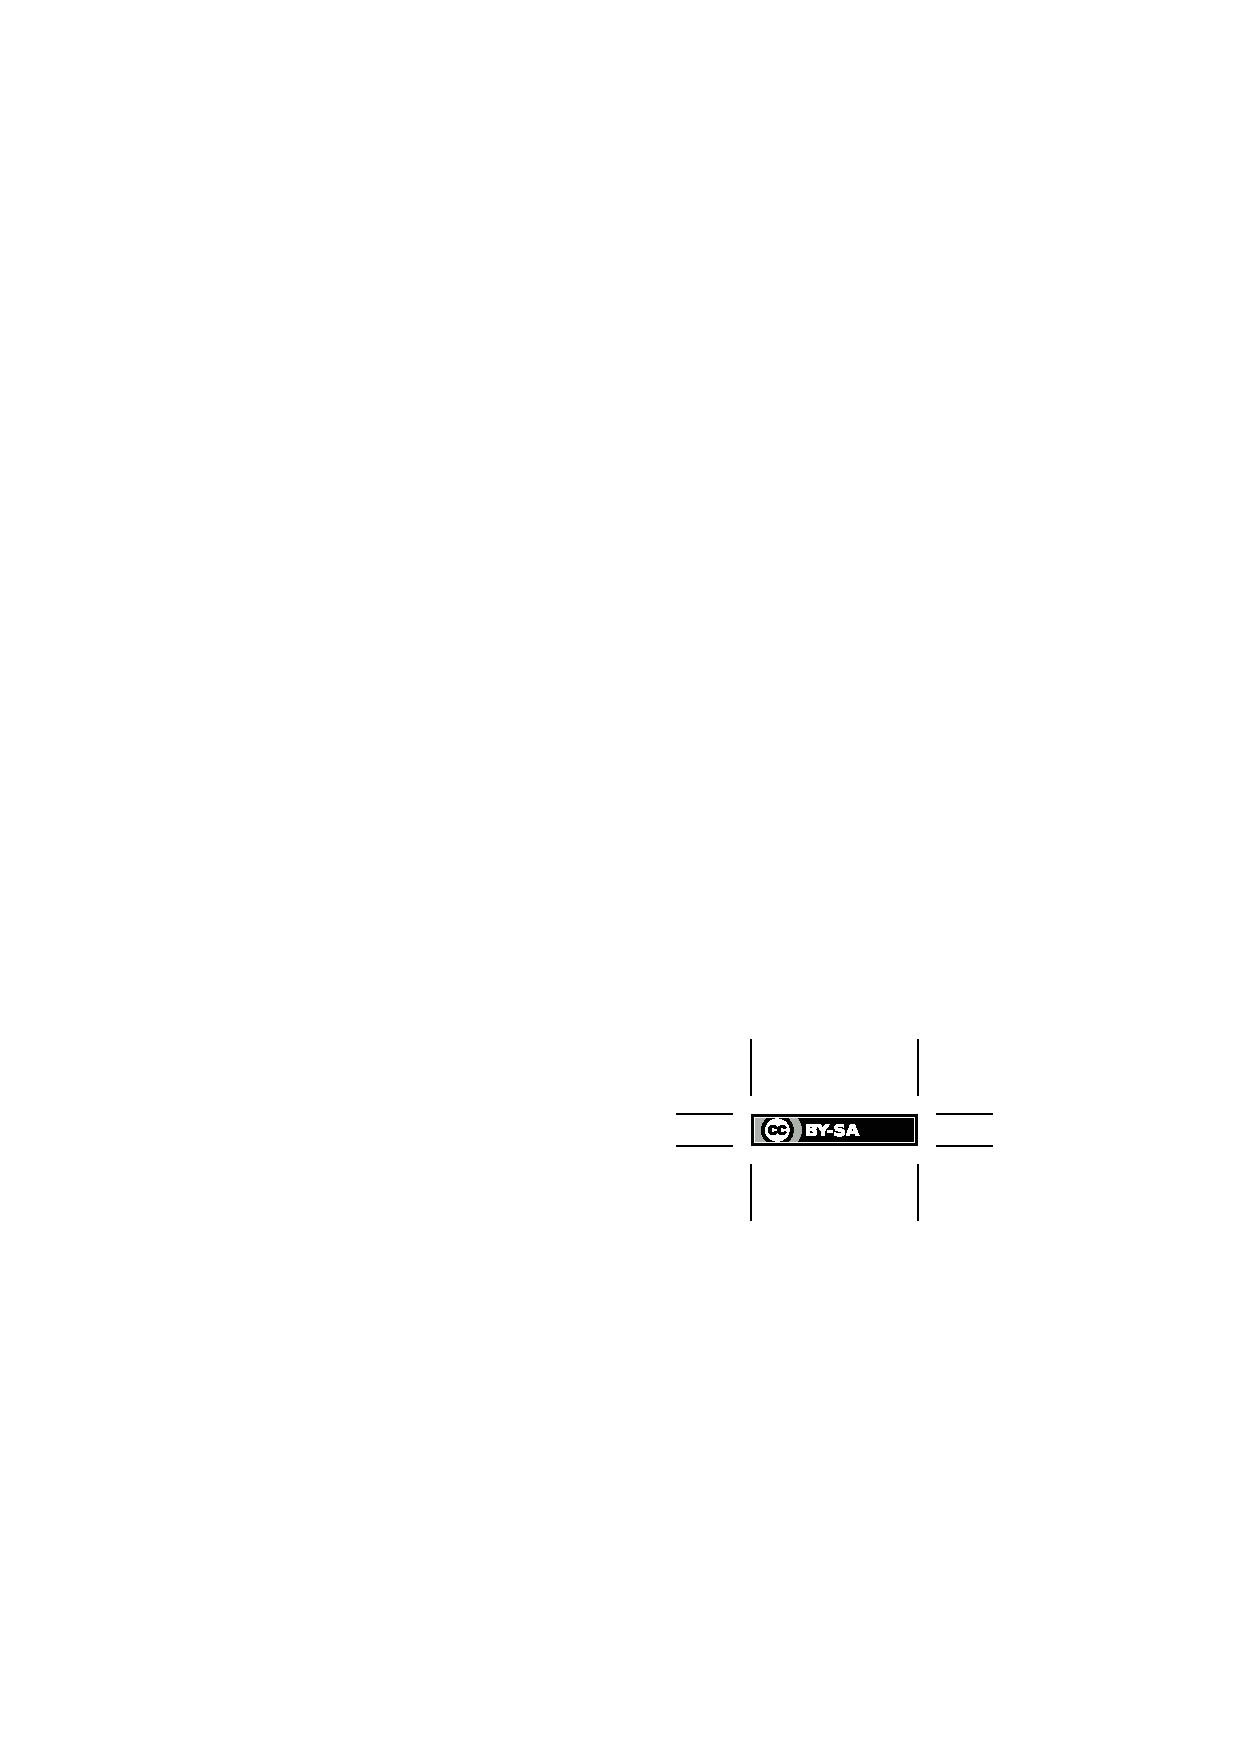
\includegraphics[scale=0.8]{by-sa}}
\end{abstract}

\tableofcontents

\clearpage

\section{Calcolo differenziale in più variabili}
% CALCOLO DIFFERENZIALE IN PIU' VARIABILI 

\begin{definition}[$ \R^n $]
	Dato il campo $ \R $ dei numeri reali, sia $ n $ un numero naturale. Una $ n $-upla di numeri reali è una sequenza $ (x_1, \ldots, x_n) $ di $ n $ numeri reali. Lo spazio di tutte le $ n $-uple di numeri reali forma uno spazio vettoriale di dimensione $ n $ su $ \R $, indicato con $ \R^n $. Indichiamo con $ \{e_1, \ldots, e_n\} $ la base canonica di $ \R^n $. \\
	Su $ \R^n $ è definito un prodotto scalare definito positivo: dati $ x \coloneqq (x_1, \ldots, x_n), \ y \coloneqq (y_1, \ldots, y_n) \in \R^n $ 
	\begin{equation}
		\sp{x}{y} \coloneqq \sum_{k = 1}^{n} x_k y_k = x_1 y_1 + \ldots + x_ny_n.
	\end{equation}
	Il prodotto scalare induce una norma su $ \R^n $:  
	\begin{equation}
		\norm{x} \coloneqq \sqrt{\sp{x}{x}} 
	\end{equation}
	La norma induce una distanza su $ \R^n $
	\begin{equation}
		d(x, y) \coloneqq \norm{x - y}
	\end{equation}
	La distanza definisce una struttura di spazio metrico e topologico in cui gli aperti sono le \emph{palle aperte} $ B_{r}(x_0) \coloneqq \{x \in \R^n : d(x, x_0) < r\} $.
\end{definition}

\begin{definition}
	Sia $ \Omega \subseteq \R^n $ e $ f \colon \Omega \to \R $ una funzione e $ x_0 \in \ouv{\Omega} $. Diciamo che $ f $ è continua in $ x_0 $ se 
	\begin{equation*}
		\forall \epsilon > 0, \ \exists \delta > 0 : \forall x \in B_\delta(x_0), \ \abs{f(x) - f(x_0)} \leq \epsilon.
	\end{equation*}
\end{definition}

\begin{definition}[derivata direzionale e parziale]
	Sia $ \Omega \subseteq \R^n $ e $ f \colon \Omega \to \R $ una funzione e $ x_0 \in \ouv{\Omega} $. 
	\begin{itemize}
		\item Dato $ v \in \R^n $ con $ \norm{v} \neq 0 $ diciamo che $ f $ è derivabile parzialmente in $ x_0 $ rispetto a $ v $ se esiste finito il limite (in 1 variabile)
		\begin{equation}
			\pd{f}{v}{(x_0)} \coloneqq \lim_{t \to 0} \frac{f(x_0 + tv) - f(x_0)}{t}.
		\end{equation}
		
		\item Dato $ i \in \{1, \ldots, n\} $ diciamo che $ f $ è derivabile parzialmente in $ x_0 $ rispetto a $ x_i $ se è derivabile direzionalmente in $ x_0 $ rispetto all'$ i $-esimo vettore $ e_i $ della base canonica di $ \R^n $ e in tale caso poniamo 
		\begin{equation}
			\pd{f}{x_i}(x_0) = f_{x_i}(x_0) \coloneqq \lim_{t \to 0} \frac{f(x_0 + te_i) - f(x_0)}{t}
		\end{equation}   
	\end{itemize}
\end{definition}

\begin{definition}[gradiente]
	Sia $ \Omega \subseteq \R^n $ e $ f \colon \Omega \to \R $ una funzione e $ x_0 \in \ouv{\Omega} $. Si dice gradiente di $ f $ nel punto $ x_0 $ il vettore che ha come componenti le derivate parziali di $ f $ nel punto $ x_0 $
	\begin{equation}
		\grad{f}(x_0) \coloneqq \left(f_{x_1}(x_0), \ldots, f_{x_n}(x_0)\right)
	\end{equation}
\end{definition}

\begin{definition}[funzione differenziabile]
	Sia $ \Omega \subseteq \R^n $ e $ f \colon \Omega \to \R^m $ una funzione e $ x_0 \in \ouv{\Omega} $. Diciamo che $ f $ è differenziabile in $ x_0 $ se esiste una applicazione lineare $ L \colon \R^n \to \R^m $ tale che 
	\begin{equation}
		f(x_0 + h) = f(x_0) + L h + o(\,\norm{h}) \quad (h \to 0)
	\end{equation}
	Nel caso $ m = 1 $, ovvero $ f \colon \Omega \to \R $, fissata una base di $ \R^n $ per il Teorema di Riesz esiste un unico $ \alpha \in \R^n $ tale che l'applicazione lineare $ L h = \sp{\alpha}{h} $ e pertanto la condizione di differenziabilità si traduce nell'esistenza di un $ \alpha \in \R^n $ tale che  
	\begin{equation}
		f(x_0 + h) = f(x_0) + \sp{\alpha}{h} + o(\,\norm{h}) \quad (h \to 0)
	\end{equation}
\end{definition}

\begin{thm}[differenziabilità, derivabilità, continuità] \label{thm:diff}
	Sia $ \Omega \subseteq \R^n $ e $ f \colon \Omega \to \R $ una funzione e $ x_0 \in \ouv{\Omega} $. Valgono le seguenti implicazioni (tutte le altre sono false)
	\begin{enumerate}[label = (\roman*)]
		\item $ f $ ammette tutte le derivate direzionali in $ x_0 $ $ \Rightarrow $ ammette tutte le derivate parziali in $ x_0 $;
		\item $ f $ è differenziabile in $ x_0 $ $ \Rightarrow $ continua in $ x_0 $ $ + $ ammette tutte le derivate direzionali in $ x_0 $ $ + $ ammette tutte le derivate parziali in $ x_0 $. \\
		In tale caso si ha $ \pd{f}{v}(x_0) = \sp{\alpha}{v} $ da cui $ \alpha = \grad{f}(x_0) $ e quindi la condizione di differenziabilità diventa
		\begin{equation*}
			f(x_0 + h) = f(x_0) + \sp{\grad{f}(x_0)}{h} + o(\,\norm{h}) \quad (h \to 0)
		\end{equation*}
	\end{enumerate}
\end{thm}
%
\begin{proof}
	\begin{enumerate}[label = (\roman*)]
		\item Ovvia. 
		\item Supponiamo $ f $ differenziabile in $ x_0 $, cioè che per $ h \to 0 $ si abbia $ f(x_0 + h) = f(x_0) + \sp{\alpha}{h} + o(\,\norm{h}) $. Così per $ h \to 0 $ si ha
		\[
			\abs{f(x_0 + h) - f(x_0)} \leq \abs{\sp{\alpha}{h}} + o(\,\norm{h}) \leq \norm{\alpha} \norm{h} + \frac{o(\,\norm{h})}{\norm{h}} \norm{h} \to 0
		\]
		da cui concludiamo che $ f $ è continua in $ x_0 $. Per quanto riguarda le derivate direzionali
		\[
			\pd{f}{v}(x_0) = \lim_{t \to 0} \frac{f(x_0 + tv) - f(x_0)}{t} = \lim_{t \to 0} 	\frac{\sp{\alpha}{tv} + o(\,\norm{tv})}{t} = \lim_{t \to 0} \left(\sp{\alpha}{v} + \frac{o(\,\norm{tv})}{\norm{tv}} \norm{v}\right) = \sp{\alpha}{v} 
		\]
		Così usando $ v = e_i $ e posto $ \alpha \coloneqq (\alpha_1, \ldots, \alpha_n) $ si ha $ f_{x_i}(x_0) = \sp{\alpha}{e_i} = \alpha_i $ da cui $ \alpha = \grad{f}(x_0) $ e in conclusione $ \pd{f}{v}(x_0) = \sp{\grad{f}(x_0)}{v} $. \qedhere
	\end{enumerate}
\end{proof}

\begin{thm}[differenziale totale] \label{thm:difftot}
	Sia $ x_0 \in \R^n $, $ \delta > 0 $ e $ f \colon B_{\delta}(x_0) \to \R $. Supponiamo che tutte le derivate parziali di $ f $
	\begin{enumerate}[label = (\roman*)]
		\item esistano in $ B_{\delta}(x_0) $
		\item siano continue in $ x_0 $
	\end{enumerate}
	Allora $ f $ è differenziabile in $ x_0 $. 
\end{thm}
%
\begin{proof}
	Fissato $ \epsilon > 0 $ vogliamo mostrare le condizione di differenziabilità in $ x_0 $, cioè che in un intorno di $ x_0 $ valga
	\[
		\abs{f(x) - f(x_0) - \sum_{k = 1}^{n} f_{x_k}(x_0)(x_k - {x_0}_k)} \leq \epsilon \norm{x - x_0}
	\]
	Essendo le derivate parziali continue in $ x_0 $, dato $ \epsilon > 0 $ esiste $ r > 0 $ (con $ r < \delta / \sqrt{2} $) tale che 
	\[
		\abs{f_{x_k}(y) - f_{x_k}(x_0)} \leq \frac{\epsilon}{n} \quad \forall y \in Q_{r}(x_0)
	\]
	dove $ Q_r(x_0) $ è il cubo $ n $-dimensionale $ Q_r(x_0) \coloneqq x_0 + (-r, r)^n $. Partiamo dall'uguaglianza valida per $ x \in Q_{r}(x_0) $
	\[
		f(x) - f(x_0) = \sum_{k = 0}^{n} f({x_0}_1, \ldots, {x_0}_{k - 1}, x_k, x_{k + 1}, \ldots, x_n) - f({x_0}_1, \ldots, {x_0}_{k - 1}, {x_0}_k, x_{k + 1}, \ldots, x_n).
	\]
	Ogni elemento della somma è l'incremento da $ {x_0}_{k} $ a $ x_k $ della funzione di una variabile 
	\[
		h_k(t) \coloneqq f({x_0}_1, \ldots, {x_0}_{k - 1}, t, x_{k + 1}, \ldots, x_n).
	\]
	Per ipotesi $ h_k(t) $ è derivabile in un intervallo aperto contenente $ {x_0}_{k} $ e $ x_k $ e 
	\[
		h'_k(t) = f_{x_k}({x_0}_1, \ldots, {x_0}_{k - 1}, t, x_{k + 1}, \ldots, x_n).
	\]
	Applicando il teorema di Lagrange otteniamo che esiste $ c_k = c_k(x_0, x) $ strettamente compreso tra $ {x_0}_{k} $ e $ x_k $ tale che
	\[
		h_k(x_k) - h_k({x_0}_k) = f_{x_k}({x_0}_1, \ldots, {x_0}_{k - 1}, c_k, x_{k + 1}, \ldots, x_n) \; (x_k - {x_0}_k)
	\]
	Così dal momento che $ y_k \coloneqq ({x_0}_1, \ldots, {x_0}_{k - 1}, c_k, x_{k + 1}, \ldots, x_n) \in Q_r(x_0) $	si ha
	\begin{align*}
		\abs{f(x) - f(x_0) - \sum_{k = 1}^{n} f_{x_k}(x_0)(x_k - {x_0}_k)} & = \abs{\sum_{k = 1}^{n} h_k(x_k) - h_k({x_0}_k) - \sum_{k = 1}^{n} f_{x_k}(x_0)(x_k - {x_0}_k)} \\
		& = \abs{\sum_{k = 1}^{n} f_{x_k}(y_k) (x_k - {x_0}_k) -  f_{x_k}(x_0)(x_k - {x_0}_k)} \\
		& \leq \sum_{k = 1}^{n} \abs{f_{x_k}(y_k) - f_{x_k}(x_0)} \abs{x_k - {x_0}_k} \leq \frac{\epsilon}{n} \sum_{k = 1}^{n} \abs{x_k - {x_0}_k} \\
		& \leq \frac{\epsilon}{n} \sum_{k = 1}^{n} \norm{x - x_0} = \frac{\epsilon}{n} \cdot n \norm{x - x_0} = \epsilon \norm{x - x_0}. \qedhere
	\end{align*} 
\end{proof}

\begin{thm}[differenziale totale "risparmioso" in $ \R^2 $]
	Sia $ (x_0, y_0) \in \R^2 $, $ \delta > 0 $ e $ f \colon (x_0 - \delta, x_0 + \delta) \times (y_0 - \delta, y_0 + \delta) \to \R $. Supponiamo che 
	\begin{enumerate}[label = (\roman*)]
		\item $ f_y(x, y) $ esiste in tutto $ (x_0 - \delta, x_0 + \delta) \times (y_0 - \delta, y_0 + \delta) $
		\item $ f_y(x, y) $ sia continua in $ (x_0, y_0) $
		\item $ f_x(x, y) $ esiste in $ (x_0, y_0) $
	\end{enumerate}
	Allora $ f $ è differenziabile in $ (x_0, y_0) $. 
\end{thm}

\begin{thm}[Schwarz 1]
	Sia $ (x_0, y_0) \in \R^2 $, $ \delta > 0 $ e $ f \colon (x_0 - \delta, x_0 + \delta) \times (y_0 - \delta, y_0 + \delta) \to \R $. Supponiamo che 
	\begin{enumerate}[label = (\roman*)]
		\item $ f_{xy}(x, y) $ e $ f_{yx}(x, y) $ esistano in $ (x_0 - \delta, x_0 + \delta) \times (y_0 - \delta, y_0 + \delta) $
		\item $ f_{xy}(x, y) $ e $ f_{yx}(x, y) $ siano continue in $ (x_0, y_0) $
	\end{enumerate}
	Allora 
	\begin{equation}
		f_{xy}(x_0, y_0) = f_{yx}(x_0, y_0)
	\end{equation}
\end{thm}

\begin{thm}[Schwarz 2]
	Sia $ (x_0, y_0) \in \R^2 $, $ \delta > 0 $ e $ f \colon (x_0 - \delta, x_0 + \delta) \times (y_0 - \delta, y_0 + \delta) \to \R $. Supponiamo che 
	\begin{enumerate}[label = (\roman*)]
		\item $ f_{xy}(x, y) $ e $ f_{yx}(x, y) $ esistano in $ (x_0 - \delta, x_0 + \delta) \times (y_0 - \delta, y_0 + \delta) $
		\item $ f_{x}(x, y) $ e $ f_{y}(x, y) $ siano differenziabili in $ (x_0, y_0) $
	\end{enumerate}
	Allora 
	\begin{equation*}
		f_{xy}(x_0, y_0) = f_{yx}(x_0, y_0)
	\end{equation*}
\end{thm}

\begin{thm}[Lagrange direzionale] \label{thm:lagrange}
	Sia $ \Omega \subseteq \R^n $, $ f \colon \Omega \to \R $ e $ a, b \in \R^n $. Supponiamo che 
	\begin{enumerate}[label = (\roman*)]
		\item tutto il segmento di estremi $ a $ e $ b $ sia contenuto in $ \ouv{\Omega} $
		\item $ f $ ammetta derivate direzionali in $ \ouv{\Omega} $
	\end{enumerate}
	Allora esiste almeno un  punto $ c \in \R^n $ nel segmento di estremi $ a $ e $ b $ tale che 
	\begin{equation}
		f(b) - f(a) = \pd{f}{v}(c) \, \norm{b - a}  \quad \text{ con } v = \frac{b - a}{\norm{b - a}}
	\end{equation}
\end{thm}
%
\begin{proof}
	Consideriamo la restrizione di $ f $ alla retta passate per $ a $ e $ b $, $ t \mapsto a + v t $ con $ v \coloneqq \dfrac{b - a}{\norm{b - a}} $ 
	\[
		\varphi(t) \coloneqq f(a + tv)
	\]
	Applicando il teorema di Lagrange alla funzione $ \varphi $ di 1 variabile
	\[
		f(b) - f(a) = \varphi(\,\norm{b - a}) - \varphi(0) = \varphi'(t_0) \norm{b - a} = \pd{f}{v}(a + t_0v) \, \norm{b - a}
	\]
	Ponendo $ c \coloneqq a + t v_0 $ otteniamo la tesi. 
\end{proof}

\begin{corollary} \label{cor:lagrange}
	Nelle stesse ipotesi del Teorema \ref{thm:lagrange} se supponiamo che $ f $ sia differenziabile in $ \ouv{\Omega} $ allora esiste almeno un  punto $ c \in \R^n $ nel segmento di estremi $ a $ e $ b $ tale che 
	\begin{equation}
		f(b) - f(a) = \sp{\grad{f}(c)}{b - a}
	\end{equation}
\end{corollary}
%
\begin{proof}
	Per il Teorema \ref{thm:diff} si ha
	\[
		f(b) - f(a) = \pd{f}{v}(c) \, \norm{b - a} = \sp{\grad{f}(c)}{\frac{b - a}{\norm{b - a}}} \, \norm{b - a} = \sp{\grad{f}(c)}{b - a} \qedhere
	\]
\end{proof}

\begin{prop}
	Sia $ D \subseteq \R^n $ un aperto convesso e $ f \colon D \to \R $. Supponiamo che 
	\begin{enumerate}[label = (\roman*)]
		\item $ f $ sia differenziabile in $ D $
		\item $ \grad{f} $ sia limitato in $ D $, cioè $ \exists M \in \R : \forall x \in D, \ \abs{\grad{f}(x)} \leq M $
	\end{enumerate}
	Allora $ f $ è $ M $-lipschitziana in $ D $.
\end{prop}

\begin{definition}[matrice Jacobiana]
	Sia $ \Omega \subseteq \R^n $ e $ f \colon \Omega \to \R^m $ una funzione differenziabile in $ x_0 \in \ouv{\Omega} $. L'applicazione lineare $ L $ data dalla condizione di differenziabilità è rappresentata dalla matrice Jacobiana
	\begin{equation}
		\jac{f}(x_0) \coloneqq \left(\dpd{f_i}{x_j}(x_0)\right)_{ij}
	\end{equation}
\end{definition}

\begin{thm}[disuguaglianza di Lagrange direzionale]
	Sia $ D \subseteq \R^n $ un insieme convesso, $ f \colon D \to \R^m $ e $ a, b \in D $. Supponiamo che $ f $ sia differenziabile in $ D $ e sia $ \jac{f} $ la sua matrice Jacobiana. Allora esiste un punto $ c $ sul segmento di estremi $ a $ e $ b $ tale che 
	\begin{equation}
		\norm{f(b) - f(a)} \leq \norm{\jac{f}(c) \ (b - a)}
	\end{equation}
\end{thm}
%
\begin{proof}
	Sia $ v \in \R^m $ e $ \varphi \colon D \to \R $ la funzione $ \varphi(x) \coloneqq \sp{f(x)}{v} $. Applicando il Corollario \ref{cor:lagrange} a tale funzione abbiamo che esiste $ c $ nel segmento di estremi $ a $ e $ b $ tale che $ \varphi(b) - \varphi(a) = \sp{\grad{\varphi}(c)}{b - a} $. Osserviamo ora che essendo $ \varphi(x) = v_1 f_1(x) + \ldots + v_m f_m(x) $ si ha pensando a $ v $ come vettore colonna
	\[
		\grad{\varphi}(x) = v_1 \grad{f_1}(x) + \ldots + v_m \grad{f_m}(x) = (\jac{f}(x))^t \, v
	\]
	da cui
	\[
		\sp{f(b) - f(a)}{v} = \sp{f(b)}{v} - \sp{f(a)}{v} = \varphi(b) - \varphi(a) = \sp{(\jac{f}(c))^t \, v}{b - a}
	\]
	Usando ora come vettore $ v = f(b) - f(a) $ otteniamo
	\begin{align*}
		\norm{f(b) - f(a)}^2 & = \sp{(\jac{f}(c))^t \, (f(b) - f(a))}{b - a} = \sp{f(b) - f(a)}{\jac{f}(c) \, (b - a)} \\
		& \leq \norm{f(b) - f(a)} \, \norm{\jac{f}(c) \, (b - a)}
	\end{align*}
	Semplificando (se possibile) concludiamo 
	\[
		\norm{f(b) - f(a)} \leq \norm{\jac{f}(c) \, (b - a)} \qedhere
	\]
\end{proof}

\begin{definition}[norma di una matrice]
	Data $ M \in \mathrm{Mat}_{n \times m}(\R) $ definiamo $ \norm{M} = \left(\sum_{i, j} M_{ij}^2\right)^{1/2} $
\end{definition}

\begin{prop}[Cauchy-Schwarz per matrici]
	Sia $ M \in \mathrm{Mat}_{n \times m}(\R) $ e $ v \in \R^m $. Allora vale la stima
	\[ \norm{Mv} \leq \norm{M} \cdot \norm{v} \]
\end{prop}
\begin{proof}
	Siano $ M_i $ le righe di $ M $. 
	\[ 
	\norm{Mv}^2 = \sum_{i=1}^{n} \sp{M_i}{v}^2 \overset{\text{\tiny C-S}}{\leq} \sum_{i=1}^{n} \norm{M_i}^2 \cdot \norm{v}^2
	    = \norm{v}^2 \sum_{i=1}^{n} \sum_{j=1}^{m} M_{ij}^2 = \norm{M}^2 \cdot \norm{v}^2. \qedhere 
	\]
\end{proof}

\begin{prop}
	Sia $ D \subseteq \R^n $ un aperto convesso e $ f \colon D \to \R $.  Supponiamo che 
	\begin{enumerate}[label = (\roman*)]
		\item $ f $ sia differenziabile in $ D $
		\item $ \jac{f} $ sia limitato in $ D $, cioè $ \exists M \in \R : \forall x \in D, \ \norm{\jac{f}(x)} \leq M $
	\end{enumerate}
	Allora $ f $ è $ M $-lipschitziana in $ D $.
\end{prop}

\begin{thm}[differenziale della funzione composta]
	Siano $ D \subseteq \R^n $, $ E \subseteq \R^m $, $ f \colon D \to \R^n $ con $ f(D) \subseteq E $ e $ g \colon E \to \R^d $. Siano inoltre $ x_0 \in \ouv{D} $ e $ y_0 = f(x_0) \in E $. Supponiamo che 
	\begin{enumerate}[label = (\roman*)]
		\item $ f $ sia differenziabile in $ x_0 $ con $ \jac{f}(x_0) $
		\item $ g $ sia differenziabile in $ y_0 $ con $ \jac{g}(y_0) $
	\end{enumerate}
	Allora $ g \circ f \colon D \to \R^d $ è differenziabile in $ x_0 $ e vale 
	\begin{equation}
		\jac{(g \circ f)}(x_0) = \jac{g}(f(x_0)) \ \jac{f}(x_0)
	\end{equation}
\end{thm}
%
\begin{proof}
	Sia $ \varphi(x) \colon D \to \R^d $ la funzione composta $ \varphi(x) \coloneqq g(f(x)) $. Per ipotesi si ha per $ h \to 0 $ e $ k \to 0 $
	\[
		f(x_0 + h) = f(x_0) + \jac{f}(x_0) \, h + o(\,\norm{h}) \qquad g(y_0 + k) = g(y_0) + \jac{g}(y_0) \, k + o(\,\norm{k}) 
	\]
	Pertanto essendo $ y_0 = f(x_0) $ e posto $ k = f(x_0 + h) - f(x_0) $ per $ h \to 0 $ si ha 
	\begin{align*}
		\varphi(x_0 + h) & = g(f(x_0 + h)) = g(f(x_0) + f(x_0 + h) - f(x_0)) \\
		& = g(f(x_0)) + \jac{g}(f(x_0)) \, (f(x_0 + h) - f(x_0)) + o(\,\norm{f(x_0 + h) - f(x_0)}) 
	\end{align*}
	Il primo termine è $ \varphi(x_0) $. Per quanto riguarda il secondo termine 
	\[
		\jac{g}(f(x_0)) \, (f(x_0 + h) - f(x_0)) = \jac{g}(f(x_0)) \, \left[\jac{f}(x_0) \, h + o(\,\norm{h})\right] = \jac{g}(f(x_0)) \, \jac{f}(x_0) \, h + o(\,\norm{h})
	\]
	Mentre il termine restante è $ o(\,\norm{h}) $: infatti
	\[
		\norm{f(x_0 + h) - f(x_0)} = \norm{\jac{f}(x_0) \, h} + o(\,\norm{h}) \leq \norm{\jac{f}(x_0)} \, \norm{h} + o(\,\norm{h}) = O(\,\norm{h})
	\]
	così $ o(\,\norm{f(x_0 + h) - f(x_0)}) = o(O(\,\norm{h})) = o(\,\norm{h}) $. Concludiamo quindi che
	\[
		\varphi(x_0 + h) = \varphi(x_0) + \jac{g}(f(x_0)) \, \jac{f}(x_0) \, h + o(\,\norm{h})
	\]
	ovvero $ \varphi $ è differenziabile in $ x_0 $ con differenziale $ \jac{g}(f(x_0)) \, \jac{f}(x_0) $. 
\end{proof}

\begin{definition}[formalismo multi-indici]
	Un multi-indice è un vettore $ p = (p_1, \ldots, p_n) $ con $ p_i \in \N $. Poniamo allora 
	\begin{itemize}
		\item $ \abs{p} = p_1 + \ldots + p_n $
		\item $ p! = p_1! \cdots p_n! $
		\item se $ x = (x_1, \ldots, x_n) \in \R^n $, allora $ x^p = x_1^{p_1} \cdots x_n^{p_n} $
		\item se $ f \colon \R^n \to \R $ allora $ D^p{f} = \dfrac{\partial^{p_1 + \ldots + p_n}{f}}{\partial{x_1^{p_1}} \cdots \, \partial{x_n^{p_n}}} $
	\end{itemize}
\end{definition}

\begin{thm}[Taylor]
	Sia $ x_0 \in \R^m $, $ \delta > 0 $, $ f \colon B_{\delta}(x_0) \to \R $ e $ n \in \N $. Allora
	\begin{equation}
		f(x_0 + h) = \sum_{\abs{p} \leq n} \frac{D^p{f}(x_0)}{p!}h^p + r_n(h) = P(h) + r_n(h)
	\end{equation}
	\begin{itemize}
		\item (\emph{Peano}) Supponiamo che 
		\begin{enumerate}[label = (\roman*)]
			\item $ f $ ammetta derivate parziali fino all'ordine $ n - 1 $ in $ B_{\delta}(x_0) $
			\item le derivate parziali fino all'ordine $ n - 1 $ siano differenziabili in $ x_0 $ (in particolare $ D^p{f}(x_0) $ esiste fino all'ordine $ \abs{p} \leq n $ e valgono i teoremi di scambio)
		\end{enumerate}
		Allora 
		\begin{equation}
			r_n(h) = o(\,\norm{h}^n)
		\end{equation}
		\item (\emph{Lagrange}) Supponiamo che 
		\begin{enumerate}[label = (\roman*)]
			\item $ f $ ammetta derivate parziali fino all'ordine $ n + 1 $ in $ B_{\delta}(x_0) $
			\item avere ipotesi sufficienti per usare i teoremi di scambio fino all'ordine $ n + 1 $ (per esempio tutte le derivate parziali fino all'ordine $ n $ sono differenziabili in $ B_{\delta}(x_0) $)
		\end{enumerate}
		Allora esiste un punto $ c \in \R^n $ sul segmento di estremi $ x_0 $ e $ x_0 + h $ (lo stesso per ogni $ p $) tale che 
		\begin{equation}
		r_n(h) = \sum_{\abs{p} = n + 1} \frac{D^p{f}(c)}{p!} h^p
		\end{equation}
	\end{itemize}
\end{thm}
%
\begin{proof}
	Dimostriamo l'enunciato per lemmi successivi.
	\begin{lemma}[derivata di un monomio]
		Se $ p $ e $ q $ sono multi-indici allora 
		\begin{equation}
			(D^q x^p)(0) = 
			\begin{cases}
				0 & \text{se $ p \neq q $} \\
				p! & \text{se $ p = q $}
			\end{cases}
		\end{equation}
	\end{lemma}
	%
	\begin{proof}[Dim]
		Siano $ p \coloneqq (p_1, \ldots, p_n) $ e $ q \coloneqq (q_1, \ldots, q_n) $. Allora se $ x \coloneqq (x_1, \ldots, x_n) $ si ha $ x^p = x_1^{p_1} \cdots x_n^{p_n} $ così
		\[
			D^q x^p = \dfrac{\partial^{q_1 + \ldots + q_n}}{\partial{x_1^{q_1}} \cdots \, \partial{x_n^{q_n}}} (x_1^{p_1} \cdots x_n^{p_n}) = \frac{\partial^{q_1}}{\partial x_1^{q_1}} x_1^{p_1} \cdots \frac{\partial^{q_n}}{\partial x_n^{q_n}} x_n^{p_n}
		\]
		da cui segue la tesi in quanto se $ y \in \R $ e $ n, m \in \N $ allora $ \od[n]{y^m}{y}(0) $ è pari a $ n! $ se $ n = m $ ed è nullo $ n \neq m $.
	\end{proof}

	\begin{lemma}[derivata di un polinomio]
		Sia $ P(x) $ un polinomio in $ n $ variabili, cioè $ P(x) \coloneqq \sum_{\abs{p} \leq d} a_p x^p $. Allora 
		\begin{equation}
			(D^pP)(0) = p! a_p.
		\end{equation}
	\end{lemma}

	\begin{lemma}[caratterizzazione del polinomio di Taylor] \label{lem:carattTaylor}
		Sia $ P(x) \coloneqq \sum_{\abs{p} \leq n} \frac{D^pf(x_0)}{p!} x^p $ il polinomio di Taylor di $ f $ di grado $ n $ centrato in $ x_0 $. Allora
		\begin{equation}
			(D^pP)(0) = (D^pf)(x_0) \quad \forall p : \abs{p} \leq n.
		\end{equation}
	\end{lemma}

	Per dimostrare Taylor-Peano e Taylor-Lagrange possiamo supporre \emph{wlog} $ x_0 = 0 $ e considerare la funzione $ \varphi(x) = f(x) - P(x) $ dove $ P(x) $ è il polinomio di Taylor di $ f $ di grado $ n $ centrato in $ 0 $ la quale per il Lemma \ref{lem:carattTaylor} soddisfa
	\begin{equation} \label{eqn:carattTaylor}
		D^p \varphi(0) = 0 \quad \forall p : \abs{p} \leq n.
	\end{equation} 

	\begin{lemma}[Peano]
		Supponiamo $ \varphi \colon B_\delta(0) \to \R $ abbia la regolarità prevista da Taylor-Peano e soddisfi \eqref{eqn:carattTaylor}. Allora 
		\[
			\lim_{x \to 0} \frac{\varphi(x)}{\norm{x}^n} = 0.
		\]
	\end{lemma}
	\begin{proof}[Dim]
		Procediamo per induzione su $ n $. Il caso $ n = 0 $ è la definizione di continuità di $ \varphi $. Il caso $ n = 1 $ è la definizione di differenziabilità. Supponiamo ora che $ \varphi $ soddisfi le ipotesi di Taylor-Peano fino all'ordine $ n + 1 $. Allora tutte le derivate parziali prime soddisfano le ipotesi di ordine $ n $ e per ipotesi induttiva sono $ o(\,\norm{x}^n) $. Ma allora anche $ \norm{\grad{\varphi}(x)} = o(\,\norm{x}^n) $. Ora per Lagrange direzionale (Teorema \ref{thm:lagrange}) vale 
		\[
			\norm{\varphi(x)} = \norm{\varphi(x) - \varphi(0)} = \norm{\sp{\grad{\varphi}(c)}{x}} \leq \norm{\grad{\varphi}(c)} \, \norm{x}
		\]
		per un qualche $ c = c(x) $ tale che $ \norm{c} < \norm{x} $. Così per $ x \to 0 $ otteniamo la tesi
		\[
			0 \leq \frac{\norm{\varphi(x)}}{\norm{x}^{n + 1}} \leq \frac{\norm{\grad{\varphi}(c)}}{\norm{c}^n} \, \frac{\norm{c}^n}{\norm{x}^n} \, \frac{\norm{x}}{\norm{x}} \leq  \frac{\norm{\grad{\varphi}(c)}}{\norm{c}^n} \to 0. \qedhere
		\]
	\end{proof}

	\begin{lemma}[Lagrange]
		Supponiamo $ \varphi \colon B_\delta(0) \to \R $ abbia la regolarità prevista da Taylor-Lagrange e soddisfi \eqref{eqn:carattTaylor}. Allora $ \forall x \in B_\delta(0) $ esiste $ c = c(x) $ sul segmento di estremi 0 e $ x $ tale che
		\[
			\varphi(x) = \sum_{\abs{p} = n + 1} \frac{D^p \varphi(c)}{p!} x^p.
		\]
	\end{lemma}
	\begin{proof}[Dim]
		Fissato $ x \in B_\delta(0) $ consideriamo la funzione di 1 variabile $ \psi \colon [-1, 1] \to \R $ data da $ \psi(t) \coloneqq \varphi(tx) $. Per tale funzione vale il Teorema di Taylor-Lagrange in 1 variabile
		\[
			\psi(t) = \sum_{k = 0}^{n} \frac{\psi^{(k)}(0)}{k!} t^k + \frac{\psi^{(n + 1)}(t_0)}{(n + 1)!}t^{n + 1}
		\]
		da cui
		\[
			\varphi(x) = \psi(1) = \sum_{k = 0}^{n} \frac{\psi^{(k)}(0)}{k!} + \frac{\psi^{(n + 1)}(t_0)}{(n + 1)!}
		\]
		Per concludere dobbiamo calcolare le derivate di $ \psi $ in funzione di quelle di $ \varphi $ usando la \emph{chain rule}. Per induzione si mostra che 
		\[
			\psi^{(k)}(t) = k! \sum_{\abs{p} = k} \frac{D^p \varphi(tx)}{p!} x^p.
		\]
		Infatti grazie alla condizione \eqref{eqn:carattTaylor} otteniamo la tesi con $ c = t_0 x $
		\[
			\varphi(x) = \sum_{k = 0}^{n} \frac{1}{k!} k! \sum_{\abs{p} = k} \frac{D^p \varphi(0)}{p!} x^p + \frac{1}{(n + 1)!} (n + 1)! \sum_{\abs{p} = n + 1} \frac{D^p \varphi(t_0x)}{p!} x^p = \sum_{\abs{p} = n + 1} \frac{D^p \varphi(t_0x)}{p!} x^p.
		\]
		Per quanto riguarda le derivate di $ \psi $ per $ k = 1 $ abbiamo $ \abs{p} = 1 $ e quindi $ p $ è della forma $ (0, \ldots, 1, \ldots, 0) $, così $ p! = 1 $, $ x^p = x_j $ e $ D^p\varphi(tx) = \pd{\varphi}{x_j}(tx) $ se $ p $ ha componente $ j $-esima non nulla. Pertanto $ \psi'(t) = \pd{\varphi}{x_1}(tx) x_1 + \ldots + \pd{\varphi}{x_m}(tx) x_m $ che è la \emph{chain rule}. Per quanto riguarda il passo induttivo si ha		
		\begin{align*}
			\psi^{(k + 1)}(t) & = \sum_{\abs{p} = k} \binom{k}{p} \dfrac{\partial^{\,\abs{p} + 1}{\varphi}}{\partial{x_1^{p_1 + 1}} \cdots \, \partial{x_m^{p_m}}} (tx)  \ x_1^{p_1 + 1} \cdots x_m^{p_m} + \ldots + \dfrac{\partial^{\,\abs{p} + 1}{\varphi}}{\partial{x_1^{p_1}} \cdots \, \partial{x_m^{p_m + 1}}} (tx)  \ x_1^{p_1} \cdots x_m^{p_m + 1} \\
			& = \sum_{q_1 + \ldots + p_m = k + 1} \binom{k}{q_1 - 1, \ldots, p_m} \dfrac{\partial^{\,q_1 + \ldots + p_m}{\varphi}}{\partial{x_1^{q_1}} \cdots \, \partial{x_m^{p_m}}} (tx)  \ x_1^{q_1} \cdots x_m^{p_m} \\
			& \quad + \ldots + \\
			& \quad + \sum_{p_1 + \ldots + q_m = k + 1} \binom{k}{p_1, \ldots, q_m - 1} \dfrac{\partial^{\,p_1 + \ldots + q_m}{\varphi}}{\partial{x_1^{p_1}} \cdots \, \partial{x_m^{q_m}}} (tx)  \ x_1^{p_1} \cdots x_m^{q_m} \\
			& = \sum_{\abs{q} = k + 1} \binom{k}{q_1 - 1, \ldots, q_m} D^q \varphi (tx)  \ x^q + \ldots + \sum_{\abs{q} = k + 1} \binom{k}{q_1, \ldots, q_m - 1} D^q \varphi (tx)  \ x^q \\
			& = \sum_{\abs{q} = k + 1} \left[\binom{k}{q_1 - 1, \ldots, q_m} + \ldots + \binom{k}{q_1, \ldots, q_m - 1}\right] D^q \varphi (tx)  \ x^q \\
			& = \sum_{\abs{q} = k + 1} \binom{k + 1}{q_1, \ldots, q_m} D^q \varphi (tx)  \ x^q \\
			& = (k + 1)!  \sum_{\abs{q} = k + 1} \frac{D^q \varphi(tx)}{q!} x^q
		\end{align*}
		Nel primo passaggio abbiamo posto $ q_j = p_j + 1 $ e nel secondo $ q = (q_1, \ldots, q_j - 1, \ldots, q_m) $		
	\end{proof}
	\phantom{\qedhere}
\end{proof}

\iffalse
Verifichiamolo per semplicità nel caso $ m = 2 $ in cui la formula diventa 
\[
\psi^{(k)}(t) = \sum_{i = 0}^{k} \binom{k}{i} \frac{\partial^k \varphi}{\partial x^i \partial y^{k - i}}(tx, ty) x^i y^{k - i}
\]
infatti
\begin{align*}
\psi^{(k + 1)}(t) & = \sum_{i = 0}^{k} \binom{k}{i} \left[\frac{\partial^{k + 1} \varphi}{\partial x^{i + 1} \partial y^{k - i}}(tx, ty) \cdot x + \frac{\partial^{k + 1} \varphi}{\partial x^{i} \partial y^{k - i + 1}}(tx, ty) \cdot y \right] x^i y^{k - i} \\
& = \sum_{i = 0}^{k}  \binom{k}{i} \frac{\partial^{k + 1} \varphi}{\partial x^{i + 1} \partial y^{k - i}}(tx, ty) x^{i + 1} y^{k - i} + \sum_{i = 0}^{k} \binom{k}{i} \frac{\partial^{k + 1} \varphi}{\partial x^{i} \partial y^{k - i + 1}}(tx, ty) \cdot x^i y^{k -i + 1} \\
(j = i + 1) & = \sum_{j = 1}^{k + 1} \binom{k}{j - 1} \frac{\partial^{k + 1} \varphi}{\partial x^{j} \partial y^{k + 1 - j}}(tx, ty) x^{j} y^{k + 1 - j} + \sum_{i = 0}^{k} \binom{k}{i} \frac{\partial^{k + 1} \varphi}{\partial x^{i} \partial y^{k + 1 - i}}(tx, ty) \cdot x^i y^{k + 1 - i} \\
& = \sum_{j = 0}^{k + 1} \binom{k}{j - 1} \frac{\partial^{k + 1} \varphi}{\partial x^{j} \partial y^{k + 1 - j}}(tx, ty) x^{j} y^{k + 1 - j} + \sum_{i = 0}^{k + 1} \binom{k}{i} \frac{\partial^{k + 1} \varphi}{\partial x^{i} \partial y^{k + 1 - i}}(tx, ty) \cdot x^i y^{k + 1 - i} \\
& = \sum_{i = 0}^{k + 1} \left[\binom{k}{i - 1} + \binom{k}{i}\right] \frac{\partial^{k + 1} \varphi}{\partial x^{i} \partial y^{k + 1 - i}}(tx, ty) x^{i} y^{k + 1 - i} \\
& = \sum_{i = 0}^{k + 1} \binom{k + 1}{i} \frac{\partial^{k + 1} \varphi}{\partial x^{i} \partial y^{k + 1 - i}}(tx, ty) x^{i} y^{k + 1 - i} \\
\end{align*}
\fi

\begin{definition}[forma quadratica]
	Una forma quadratica in $ n $ variabili una somma di monomi di secondo grado
	\begin{equation}
		q(x) \coloneqq \sum_{\abs{p} = 2} a_p x^p.
	\end{equation}
	A ogni forma quadratica possiamo associare una matrice $ M $ simmetrica $ n \times n $ tale che 
	\begin{equation*}
		q(x) = x^t M x.
	\end{equation*}
	Diciamo inoltre che una forma quadratica di variabile reale è 
	\begin{itemize}
		\item \emph{definita positiva} se $ \forall x \neq 0, \ q(x) > 0 $
		\item \emph{semi-definita positiva} se $ \forall x, \ q(x) \geq 0 $
		\item \emph{definita negativa} se $ \forall x \neq 0, \ q(x) < 0 $
		\item \emph{semi-definita negativa} se $ \forall x, \ q(x) \leq 0 $
		\item \emph{indefinita} se $ \exists v, w : \ q(v) > 0, \ q(w) < 0 $
	\end{itemize}
\end{definition}

\begin{prop} \label{prop:formquadratica}
	Sia $ q(x) $ una forma quadratica di variabile reale definita positiva. Allora esiste $ m > 0 $ tale che 
	\begin{equation}
		q(x) \geq m \norm{x}^2 \quad \forall x \in \R^n
	\end{equation}
	Similmente se $ q(x) $ è definita negativa allora esiste $ m > 0 $ tale che 
	\begin{equation}
		q(x) \leq -m \norm{x}^2 \quad \forall x \in \R^n
	\end{equation}
\end{prop}
%
\begin{proof}
	Supponiamo $ q $ definita positiva e sia $ M $ la matrice di $ q $. Mostriamo la tesi con $ m \coloneqq \min{\{\lambda_1,\ldots, \lambda_n\}} > 0 $ dove $ \lambda_1, \ldots, \lambda_n $ sono gli autovalori di $ M $. Essendo $ M $ reale e simmetrica essa è diagonalizzabile mediante una matrice ortonormale, cioè esiste una matrice $ A $ tale che $ A M A^{-1} = A M A^t = D $ con $ D $ matrice diagonale. Allora
	\[
		q(x) = x^t M x = x^t A^t D A x = (Ax)^t D Ax \geq m \norm{Ax}^2 = m \norm{x}^2
	\]
	La disuguaglianza segue dal fatto che se $ D $ è matrice diagonale, per ogni $ v \in \R^n $ si ha
	\[
		v^t D v = \lambda_1 v_1^2 + \ldots + \lambda_n v_n^2 \geq m (v_1^2 + \ldots + v_n^2) = m \norm{v}^2
	\]
	Mentre l'ultima uguaglianza segue da 
	\[
		\norm{Ax}^2 = (Ax)^t Ax = x^t A^t A x = x^t \Id x = x^t x = \norm{x}^2. \qedhere
	\]
\end{proof}

\begin{definition}[matrice Hessiana]
	Sia $ \Omega \subseteq \R^n $ e $ f \colon \Omega \to \R $ una funzione e $ x_0 \in \ouv{\Omega} $. Si dice matrice Hessiana di $ f $ nel punto $ x_0 $ la matrice che ha come componenti le derivate parziali seconde di $ f $ nel punto $ x_0 $
	\begin{equation}
		\hess{f}(x_0) \coloneqq \left(\dmd{f}{2}{x_i}{}{x_j}{} (x_0)\right)_{ij} 
	\end{equation}
	Osserviamo che lo sviluppo di Taylor di ordine 2 si può scrivere in termini della matrice Hessiana (matrice associata alla forma quadratica del secondo ordine)
	\begin{equation}
		f(x_0 + h) = f(x_0) + \sp{\grad{f}(x_0)}{h} + \frac{1}{2} h^t \, \hess{f}(x_0) \, h + r_2(h)
	\end{equation}
\end{definition}

\begin{thm}[punti stazionari e Hessiana]
	Sia $ x_0 \in \R^n $, $ \delta > 0 $ e $ f \colon B_{\delta}(x_0) \to \R $. Supponiamo che 
	\begin{enumerate}[label = (\roman*)]
		\item $ f $ ammetta derivate parziali fino all'ordine 2 continue in $ B_{\delta}(x_0) $
		\item $ x_0 $ è un punto stazionario per $ f $, cioè $ \grad{f}(x_0) = 0 $
	\end{enumerate}
	Allora valgono le seguenti implicazioni
	\begin{itemize}
		\item $ \hess{f}(x_0) $ è definita positiva $ \Rightarrow $ $ x_0 $ è punto di minimo locale
		\item $ \hess{f}(x_0) $ è definita negativa $ \Rightarrow $ $ x_0 $ è punto di massimo locale
		\item $ \hess{f}(x_0) $ è indefinita $ \Rightarrow $ $ x_0 $ non è né massimo né minimo locale
		\item $ \hess{f}(x_0) $ è semi-definita $ \Rightarrow $ ?
	\end{itemize}
\end{thm}
%
\begin{proof}
	Supponiamo $ \hess{f}(x_0) $ definita positiva e sia $ q(h) $ la forma quadratica associata. Per la Proposizione \ref{prop:formquadratica} $ \exists m > 0 : q(h) \geq m \norm{h}^2 $ per ogni $ h $. Così per Taylor-Peano
	\begin{gather*}
		f(x_0 + h) = f(x_0) + \sp{\grad{f}(x_0)}{h} + \frac{1}{2} q(h) + o(\,\norm{h}^2) \geq f(x_0) + m \norm{h}^2 + o(\,\norm{h}^2) \\
		\Rightarrow \quad f(x_0 + h) - f(x_0) \geq \norm{h}^2 \left(m + \frac{o(\,\norm{h}^2)}{\norm{h}^2}\right)
	\end{gather*}
	Dal momento che $ \frac{o(\,\norm{h}^2)}{\norm{h}^2} \to 0 $ per $ h \to 0 $ sappiamo che $ \exists \delta_0 \in (0, \delta) $ tale che $ m + \frac{o(\,\norm{h}^2)}{\norm{h}^2} \geq \frac{m}{2} > 0 $ quando $ \norm{h} \leq \delta_0 $. Da questo concludiamo che 
	\[
		f(x_0 + h) > f(x_0) \quad \forall h : 0 < \norm{h} \leq \delta_0
	\]
	ovvero $ x_0 $ è punto di minimo locale per $ f $. \\
	Se $ \hess{f}(x_0) $ è definita negativa procediamo come sopra usando il fatto che $ \exists m > 0 : q(h) \leq -m \norm{h}^2 $ per concludere che $ x_0 $ è punto di massimo locale usando. \\
	Supponiamo $ \hess{f}(x_0) $ è indefinita e sia $ q(h) $ la forma quadratica ad essa associa. Allora sappiamo che $ \exists v \in \R^n : q(v) < 0 $ e $ \exists w \in \R^n : q(w) > 0 $. Allora per Taylor-Peano in un opportuno intorno di $ x_0 $ ($ t = 0 $), da un lato 
	\[
		f(x_0 + tv) - f(x_0) = \frac{1}{2} q(tv) + o(\norm{tv}^2) = t^2 \left(\frac{1}{2}q(v) + \norm{v}^2 \frac{o(t^2\norm{v}^2)}{t^2\norm{v}^2}\right) < 0 \quad \Rightarrow \quad f(x_0 + tv) < f(x_0)
	\]
	mentre dall'altro
	\[
		f(x_0 + tw) - f(x_0) = \frac{1}{2} q(tw) + o(\norm{tw}^2) = t^2 \left(\frac{1}{2}q(v) + \norm{w}^2 \frac{o(t^2\norm{w}^2)}{t^2\norm{w}^2}\right) > 0 \quad \Rightarrow \quad f(x_0 + tw) > f(x_0)\qedhere
	\]
\end{proof}

\begin{thm}[degli zeri generalizzato]
	Sia $ \Omega \subseteq \R^n $ e $ f \colon \Omega \to \R $ una funzione. Supponiamo che  
	\begin{enumerate}[label = (\roman*)]
		\item $ \Omega $ sia connesso
		\item $ f $ sia continua
	\end{enumerate}
	Allora l'immagine di $ \Omega $ secondo $ f $, cioè $ f(\Omega) $, è connesso.
\end{thm}
%
\begin{proof}
	Supponiamo per assurdo che $ f(\Omega) $ sia sconnesso, ovvero esistano $ A, B \subseteq f(\Omega) $ aperti in $ f(\Omega) $ tali che $ A, B \neq \emptyset $, $ A \cap B = \emptyset $ e $ A \cup B = f(\Omega) $. Ma allora essendo $ f $ continua $ f^{-1}(A) $ e $ f^{-1}(B) $ sono aperti in $ \Omega $ (controimmagine continua di un aperto), sono non vuoti (sottoinsiemi dell'immagine) e risulta $ f^{-1}(A) \cap f^{-1}(B) = f^{-1}(A \cap B) = f^{-1}(\emptyset) = \emptyset $ e $ f^{-1}(A) \cup f^{-1}(B) = f^{-1}(A \cup B) = f^{-1}(f(\Omega)) = \Omega $, ovvero $ \Omega $ è sconnesso da cui l'assurdo. 
\end{proof}

\begin{lemma} \label{lem:succminim}
	Sia $ \Omega \subseteq \R^n $ e $ f \colon \Omega \to \R $ una funzione continua. Allora esiste una successione minimizzante, ovvero detto $ I \coloneqq \inf_{\Omega}f $, esiste $ (x_n)_{n \in \N} \subseteq \Omega : f(x_n) \to I $. Enunciato analogo vale per l'estremo superiore.
\end{lemma}
%
\begin{proof}
	Distinguiamo due casi. Se $ I = -\infty $ allora $ f $ non è inferiormente limitata e pertanto per ogni $ n \in \N $ esiste $ y_n \in f(\Omega) : y_n < -n $. Per definizione di immagine esiste $ x_n \in \Omega : f(x_n) = y_n $ così per confronto $ f(x_n) \to -\infty $. Se $ I \in \R $ allora $ \forall \epsilon > 0 $ esiste $ y \in f(\Omega) : I \leq y < I + \epsilon $. Posto allora $ \epsilon = 1/n $ per ogni $ n \in \N $ abbiamo che $ \exists y_n \in f(\Omega) : I \leq y_n < I + 1/n $. Per definizione di immagine esiste $ x_n \in \Omega : f(x_n) = y_n $ così per confronto $ f(x_n) \to I $.
\end{proof}

\begin{thm}[Weierstrass] \label{thm:Weierstrass}
	Sia $ K \subseteq \R^n $ e $ f \colon K \to \R $. Supponiamo che
	\begin{enumerate}[label = (\roman*)]
		\item $ K $ sia compatto e $ K \neq \emptyset $
		\item $ f $ sia continua
	\end{enumerate}
	Allora esistono $ \max_K f $ e $ \min_K f $	(se mi basta il minimo è sufficiente che $ f $ sia semi-continua inferiormente). 
\end{thm}
%
\begin{proof}
	Supponiamo $ f $ semi-continua inferiormente. Sia $ I \coloneqq \inf_K f \in \R \cup \{-\infty\} $. Per il Lemma \ref{lem:succminim} esiste $ (x_n)_{n \in \N} \subseteq K $ tale che $ f(x_n) \to I $ ed essendo $ K $ compatto esiste $ x_0 \in K $ e una sottosuccessione $ (x_{n_k}) \subseteq K $ tale che $ x_{n_k} \to x_0 $. Così per la semi-continuità inferiore
	\[
		I \leq f(x_0) \leq \liminf_{k \to +\infty} f(x_{n_k}) = \liminf_{n \to +\infty} f(x_n) = \lim_{n \to +\infty} f(x_n) = I
	\]
	In conclusione $ f(x_0) = I $ da cui $ I \in \R $, $ I = \min_K f $ e $ x_0 $ è punto di minimo.
\end{proof}

\begin{thm}[Weierstrass generalizzato 1] \label{thm:Weierstrassgen1}
	Sia $ D \subseteq \R^n $ con $ D \neq \emptyset $ e $ f \colon D \to \R $. Supponiamo che
	\begin{enumerate}[label = (\roman*)]
		\item esista un sottolivello non vuoto contenuto in un compatto, cioè
		\[
			\exists M \in \R, \ \exists K \subseteq D \text{ compatto} : \ \emptyset \neq \{x \in D : f(x) \leq M\} \subseteq K
		\]
		\item $ f $ sia continua (semi-continua inferiormente)
	\end{enumerate}
	Allora esiste $ \min_D f $. 
\end{thm}
%
\begin{proof}
	Per il Teorema \ref{thm:Weierstrass}, $ f $ ammette minimo in $ K $ e sia $ x_0 \in K $ un corrispondente punto di minimo. Allora $ x_0 $ è punto di minimo in $ D $: infatti se $ x \in D $
	\begin{itemize}
		\item $ x \in K \Rightarrow f(x) \geq f(x_0) $
		\item $ x \notin K \Rightarrow f(x) > M \geq f(x_0) $
	\end{itemize}
	e pertanto in ogni caso $ f(x) \geq f(x_0) $. 
\end{proof}

\begin{thm}[Weierstrass generalizzato 2]
	Sia $ f \colon \R^n \to \R $. Supponiamo che 
	\begin{enumerate}[label = (\roman*)]
		\item $ \displaystyle{\lim_{\norm{x} \to +\infty}} f(x) = +\infty $
		\item $ f $ sia continua (semi-continua inferiormente)
	\end{enumerate}
	Allora esiste $ \min f $. 
\end{thm}
%
\begin{proof}
	Consideriamo il sottolivello $ \{x \in \R^n : f(x) \leq f(0)\} $. Tale insieme è 
	\begin{itemize}
		\item non vuoto
		\item chiuso (per la semi-continuità inferiore se $ (x_n) $ è una successione nel sottolivello tale che $ x_n \to x_0 $, allora $ f(x_0) \leq \liminf_{n \to +\infty} f(x_n) \leq f(0) $)
		\item limitato (per definizione di limite $ \exists R > 0 : \forall x \in \R^n : \norm{x} \geq R, \ f(x) \geq f(0) + 42 $ e quindi il sottolivello è contenuto in $ B_R(0) $)
	\end{itemize}
	Essendo quindi il sottolivello compatto per il Teorema \ref{thm:Weierstrassgen1} $ f $ ha minimo su $ \R^n $. 
\end{proof}

\begin{thm}[funzione implicita] \label{thm:funzimpl}
	Sia $ \Omega \subseteq \R^n $ aperto, $ f \colon \Omega \to \R $ e $ (x_0, y_0) \in \Omega $ con $ x_0 \in \R^{n - 1} $ e $ y_0 \in \R $ (nel seguito i punti di $ \Omega $ vengono indicati come $ (x, y) $ dove si intende $ x \in \R^{n - 1} $ e $ y \in \R $). Supponiamo che
	\begin{enumerate}[label = (\roman*)]
		\item $ f(x_0, y_0) = 0 $ e sia $ V \coloneqq \{(x, y) \in \Omega : f(x, y) = 0\} $ 
		\item $ f $ sia continua in $ \Omega $ 
		\item $ f_{x_n}(x, y) $ esiste ed è continua in $ \Omega $ 
		\item $ f_{x_n}(x_0, y_0) \neq 0 $
	\end{enumerate}
	Allora
	\begin{enumerate}[label = (\arabic*)]
		\item Esistono $ \rho > 0 $, $ r > 0 $ ed un'unica funzione $ \varphi \colon \overline{B}_{\rho}(x_0) \to [y_0 - r, y_0 + r] $ tale che
		\[
			V \cap (\overline{B}_{\rho}(x_0)  \times [y_0 - r, y_0 + r]) = \{(x, y) \in \Omega : x \in \overline{B}_{\rho}(x_0) , \ y = \varphi(x)\}
		\]
		\item La funzione $ \varphi $ è continua in $ \overline{B}_{\rho}(x_0)  $
		\item Se $ f $ è di classe $ C^1 $ in $ \Omega $, allora $ \varphi $ ammette derivate parziali in $ B_{\rho}(x_0)  $ date per ogni $ i \in \{1, \ldots, n - 1\} $ da
		\begin{equation}
			\varphi_{x_i}(x) = - \frac{f_{x_i}(x, \varphi(x))}{f_{x_n}(x, \varphi(x))} \qquad \forall x \in B_{\rho_0}(x_0)
		\end{equation}
		\item Se $ f $ è i classe $ C^k $ in $ \Omega $ allora $ \varphi $ è di classe $ C^k $
	\end{enumerate} 
\end{thm}

\begin{definition}[min/max vincolato]
	Sia $ \Omega \subseteq \R^n $, $ f \colon \Omega \to \R $ e $ g \colon \Omega \to \R $. Sia $ V $ il luogo degli zeri di $ g $ cioè 
	\begin{equation}
		V \coloneqq \{x \in \Omega : \ g(x) = 0\}
	\end{equation}
	Diciamo che $ x_0 \in V $ è punto di minimo locale per $ f $ ristretta/vincolata a $ V $ se 
	\begin{equation*}
		\exists r > 0 : \ \forall x \in V \cap B_r(x_0), \ f(x) \geq f(x_0)
	\end{equation*}
	Analogamente per il massimo.
\end{definition}

\begin{thm}[moltiplicatori di Lagrange: 1 moltiplicatore]
	Sia $ \Omega \subseteq \R^n $ aperto, $ f \colon \Omega \to \R $ e $ g \colon \Omega \to \R $ di classe $ C^1 $. Sia inoltre $ V $ il luogo degli zeri di $ g $. Supponiamo che $ x_0 \in V $ sia punto mi massimo o minimo vincolato per $ f $ su $ V $. Allora si ha almeno una delle seguenti possibilità
	\begin{enumerate}[label = (\roman*)]
		\item $ \grad{g}(x_0) = 0 $
		\item $ \grad{f}(x_0) $ è multiplo di $ \grad{g}(x_0) $, cioè 
		\begin{equation}
			\exists \lambda \in \R : \grad{f}(x_0) = \lambda \grad{g}(x_0)
		\end{equation}
	\end{enumerate}
\end{thm}
%
\begin{proof}
	(caso $ n = 2 $). Siamo in $ \R^2 $, il punto è $ (x_0, y_0) $, il vincolo è $ g(x, y) = 0 $. Se $ \grad{g}(x_0, y_0) $ allora siamo nel caso (i). Supponiamo quindi $ \grad{g}(x_0, y_0) \neq 0 $, \emph{wlog} $ g_y(x_0, y_0) \neq 0 $. Allora per il Teorema \ref{thm:funzimpl} esistono $ \rho > 0 $, $ r > 0 $ e un'unica $ \gamma \colon [x_0 - \rho, x_0 + \rho] \to [y_0 - r, y_0 + r] $ tale che 
	\[
		V \cap ([x_0 - \rho, x_0 + \rho] \times [y_0 - r, y_0 + r]) = \{(x, \gamma(x)) : x \in [x_0 - \rho, x_0 + \rho]\}.
	\]
	Consideriamo allora la funzione $ \varphi \colon [x_0 - \rho, x_0 + \rho] \to \R $ definita da $ \varphi(x) \coloneqq f(x, \varphi(x)) $. Per ipotesi sappiamo che $ x_0 $ è punto di max/min per $ \varphi $, dunque $ \varphi'(x_0) = 0 $. D'altra parte per la \emph{chain rule} e per la formula data dal teorema di funzione implicita
	\[
		\varphi'(x) = f_x(x, \gamma(x)) + f_y(x, \gamma(x)) \left(- \frac{g_x(x, \gamma(x))}{g_y(x, \gamma(x))}\right)
	\]
	così essendo $ y_0 = \gamma(x_0) $
	\[
		0 = \varphi'(x_0) = f_x(x_0, y_0) - \frac{f_y(x_0, y_0)}{g_y(x_0, y_0)} g_x(x_0, y_0).
	\]
	Posto allora $ \lambda \coloneqq \dfrac{f_y(x_0, y_0)}{g_y(x_0, y_0)} $ otteniamo la tesi
	\[
		f_x(x_0, y_0) = \lambda g_x(x_0, y_0), \quad f_y(x_0, y_0) = \lambda g_y(x_0, y_0) \quad \Rightarrow \quad \grad{f}(x_0, y_0) = \lambda \grad{g}(x_0, y_0) \qedhere
	\]
\end{proof}
\begin{proof}
	(caso $ n $ generico). Siamo in $ \R^n $, il punto è $ x_0 \coloneqq ({x_0}_1, \ldots, {x_0}_n) $, il vincolo è $ g(x_1, \ldots, x_n) = 0 $. Se $ \grad{g}(x_0) $ allora siamo nel caso (i). Supponiamo quindi $ \grad{g}(x_0) \neq 0 $, \emph{wlog} $ g_{x_n}(x_0) \neq 0 $. Nel seguito indichiamo i punti come $ (\bar{x}, \bar{y}) $ con $ \bar{x} \in \R^{n - 1} $ e $ \bar{y} \in \R $ e poniamo $ \bar{x}_0 = ({x_0}_1, \ldots, {x_0}_n) $ e $ \bar{y}_0 = {x_n}_0 $ così $ x_0 = (\bar{x}_0, \bar{y}_0) $. Allora per il Teorema \ref{thm:funzimpl} esistono $ \rho > 0 $, $ r > 0 $ e un'unica $ \gamma \colon \overline{B}_\rho(\bar{x}_0) \to [\bar{y}_0 - r, \bar{y}_0 + r] $ tale che 
	\[
		V \cap (\overline{B}_\rho(\bar{x}_0) \times [\bar{y}_0 - r, \bar{y}_0 + r]) = \{(\bar{x}, \gamma(\bar{x})) : \bar{x} \in \overline{B}_\rho(\bar{x}_0)\}.
	\]
	Consideriamo allora la funzione $ \varphi \colon \overline{B}_\rho(\bar{x}_0) \to \R $ definita da $ \varphi(\bar{x}) \coloneqq f(\bar{x}, \gamma{(\bar{x})}) $. Per ipotesi sappiamo che $ \bar{x}_0 $ è punto di max/min per $ \varphi $, dunque $ \varphi'(\bar{x}_0) = 0 $. D'altra parte per la \emph{chain rule} e per la formula data dal teorema di funzione implicita
	\[
		\varphi_{x_i}(\bar{x}) = f_{x_i}(\bar{x}, \gamma(\bar{x})) + f_{x_n}(\bar{x}, \gamma(\bar{x})) \left(- \frac{g_{x_i}(\bar{x}, \gamma(\bar{x}))}{g_{x_n}(\bar{x}, \gamma(\bar{x}))}\right) \quad \forall i \in \{1, \ldots, n - 1\}
	\]
	così essendo $ \bar{y}_0 = \gamma(\bar{x}_0) $
	\[
		0 = \varphi_{x_i}(\bar{x}_0) = f_{x_i}(\bar{x}_0, \bar{y}_0) - \frac{f_{x_n}(\bar{x}_0, \bar{y}_0)}{g_{x_n}(\bar{x}_0, \bar{y}_0)} g_{x_i}(\bar{x}_0, \bar{y}_0) \quad \forall i \in \{1, \ldots, n - 1\}.
	\]
	Posto allora $ \lambda \coloneqq \dfrac{f_{x_n}(\bar{x}_0, \bar{y}_0)}{g_{x_n}(\bar{x}_0, \bar{y}_0)} $ otteniamo la tesi
	\begin{gather*}
		f_{x_i}(\bar{x}_0, \bar{y}_0) = \lambda g_{x_i}(\bar{x}_0, \bar{y}_0) \ \quad \forall i \in \{1, \ldots, n - 1\}, \quad f_{x_n}(\bar{x}_0, \bar{y}_0) = \lambda g_{x_n}(\bar{x}_0, \bar{y}_0) \\
		\Rightarrow \quad \grad{f}(x_0) = \lambda \grad{g}(x_0) \qedhere
	\end{gather*}
\end{proof}

\begin{thm}[funzione implicita con $ k $ equazioni]
	Sia $ \Omega \subseteq \R^n $ aperto, $ f \colon \Omega \to \R^k $ e $ (x_0, y_0) \in \Omega $ con $ x_0 \in \R^{n - k} $ e $ y_0 \in \R^k $ (nel seguito i punti di $ \Omega $ vengono indicati come $ (x, y) $ dove si intende $ x \in \R^{n - k} $ e $ y \in \R^k $). Supponiamo che
	\begin{enumerate}[label = (\roman*)]
		\item $ f(x_0, y_0) = 0 $ e sia $ V \coloneqq \{(x, y) \in \Omega : f(x, y) = 0\} $
		\item $ f $ sia continua in $ \Omega $
		\item $ \jac_y{f}(x, y) $ (matrice $ k \times k $ delle derivate di $ f $ rispetto alle ultime $ k $ variabili) esista e sia continuo in $ \Omega $
		\item $ \jac_y{f}(x_0, y_0) $ sia invertibile
	\end{enumerate}
	Allora
	\begin{enumerate}[label = (\arabic*)]
		\item Esistono $ \rho > 0 $, $ r > 0 $ ed un'unica funzione $ \varphi \colon \overline{B}_{\rho}(x_0) \to \overline{B}_{r}(y_0) $ tale che
		\[
		V \cap (\overline{B}_{\rho}(x_0) \times \overline{B}_{r}(y_0)) = \{(x, y) \in \Omega : x \in \overline{B}_{\rho}(x_0) , \ y = \varphi(x)\}
		\]
		\item La funzione $ \varphi $ è continua in $ \overline{B}_{\rho}(x_0) $
		\item Se $ f $ è differenziabile in $ (x_0, y_0) $ allora $ \varphi $ è differenziabile in $ x_0 $ e vale
		\begin{equation}
			\jac_x{\varphi}(x_0) = - \left[\jac_y{f}(x_0, y_0)\right]^{-1} \jac_x{f}(x_0, y_0)
		\end{equation}
		\item Se $ f $ è i classe $ C^k $ in $ \Omega $ allora $ \varphi $ è di classe $ C^k $ 
	\end{enumerate} 
\end{thm}

\begin{thm}[moltiplicatori di Lagrange: $ k $ moltiplicatori]
	Sia $ \Omega \subseteq \R^n $ aperto, $ f \colon \Omega \to \R $ di classe $ C^1 $ e $ k < n $. Siano $ g_1, \ldots, g_k \colon \Omega \to \R $ di classe $ C^1 $ e $ V $ il luogo degli zeri di $ g_1, \ldots, g_k $ cioè 
	\begin{equation*}
		V \coloneqq \{x \in \Omega : g_1(x) = \ldots = g_k(x) = 0\}.
	\end{equation*}
	Supponiamo che $ x_0 \in V $ sia punto mi massimo o minimo vincolato per $ f $ su $ V $. Allora si ha almeno una delle seguenti possibilità
	\begin{enumerate}[label = (\roman*)]
		\item $ \grad{g_1}(x_0), \ldots, \grad{g_k}(x_0) $ sono linearmente dipendenti
		\item $ \grad{f}(x_0) $ è combinazione lineare di $ \grad{g_1}(x_0), \ldots, \grad{g_k}(x_0) $, cioè 
		\begin{equation}
			\exists \lambda_1, \ldots, \lambda_k \in \R : \grad{f}(x_0) = \lambda_1 \grad{g_1}(x_0) + \ldots +\lambda_k \grad{g_k}(x_0)
		\end{equation}
	\end{enumerate}
\end{thm}

\begin{prop}
	Sia $ \Omega \subseteq \R^n $ e $ f \colon \Omega \to \R $. Sia $ x_0 \in \Omega $ un punto di minimo o massimo per $ f $. Allora $ x_0 $ appartiene ad una delle seguenti categorie
	\begin{itemize}
		\item $ x_0 $ è un punto stazionario interno, cioè $ x_0 \in \ouv{\Omega} $ e $ \grad{f}(x_0) = 0 $
		\item $ x_0 $ è un punto singolare interno, cioè $ x_0 \in \ouv{\Omega} $ e $ \grad{f}(x_0) $ non esiste
		\item $ x_0 $ è un punto di bordo, cioè $ x_0 \in \partial \Omega $
	\end{itemize}
\end{prop}
\clearpage

\section{Calcolo integrale in più variabili}
% 	CALCOLO INTEGRALE IN PIU' VARIABILI

\subsection{Integrali doppi}

\begin{definition}[funzione integrabile su $ \R^2 $ alla Darboux "unrestricted"]
	Sia $ f \colon \R^2 \to \R $ una funzione
	\begin{enumerate}[label = (\roman*)]
		\item limitata
		\item nulla al di fuori di un limitato 
	\end{enumerate}
	Procediamo per passi successivi:
	\begin{enumerate}
		\item \emph{Caso banale}. Sia $ R \coloneqq [a, b] \times [c, d] $ un rettangolo e $ \lambda \in \R $. Supponiamo che 
		\begin{equation*}
			f(x, y) \coloneqq \lambda \varphi_{R}(x, y) = 
			\begin{cases}
				\lambda & \text{se $ (x, y) \in R $} \\
				0 & \text{se $ (x, y) \notin R $}
			\end{cases}
		\end{equation*}
		Poniamo allora 
		\begin{equation}
			\iint_{\R^2} f(x, y) \dif{x} \dif{y} \coloneqq \lambda (b - a) (d - c)
		\end{equation}
		
		\item \emph{Caso semi-banale}. $ f $ è una \emph{step-function}, cioè
		\begin{equation*}
			f(x, y) \coloneqq \sum_{i = 1}^{n} \lambda_i \varphi_{R_i}(x, y)
		\end{equation*}
		dove $ \lambda_i \in \R $ e $ R_i \coloneqq [a_i, b_i] \times [c_i, d_i] $. Poniamo allora 
		\begin{equation}
			\iint_{\R^2} f(x, y) \dif{x} \dif{y} \coloneqq \sum_{i = 1}^{n} \lambda_i (b_i - a_i) (d_i - c_i)
		\end{equation}
		\textbf{Fatto 1}. Se la stessa funzione si scrive in due modi diversi come combinazione di caratteristiche, allora l'integrale definito nei due modi diversi coincide. \\
		\textbf{Fatto 2}. Ogni \emph{step-function} può essere pensata come definita come combinazione lineare di caratteristiche di rettangoli senza parti interne in comune. 
		
		\item \emph{Caso generale}. $ f $ è una funzione qualunque che soddisfa le ipotesi. Definiamo l'integrale superiore e inferiore di $ f $ come 
		\begin{gather*}
			I^+(f) \coloneqq \inf{\left\{\iint_{\R^2} \varphi(x, y) \dif{x} \dif{y} : \varphi \text{ è una \emph{step-function} e } \forall (x, y) \in \R^2, \ \varphi(x, y) \geq f(x, y)\right\}} \\
			I^-(f) \coloneqq \sup{\left\{\iint_{\R^2} \psi(x, y) \dif{x} \dif{y} : \psi \text{ è una \emph{step-function} e } \forall (x, y) \in \R^2, \ \psi(x, y) \leq f(x, y)\right\}}
		\end{gather*}
		\textbf{Fatto 1}. $ I^+(f) $ e $ I^-(f) $ esistono sempre e vale la relazione $ I^-(f) \leq I^+(f) $\\
		\textbf{Fatto 2}. Se $ \varphi_1 $ e $ \varphi_2 $ sono due \emph{step-functions} tali che $ \forall (x, y) \in \R^2 : \varphi_1(x, y ) \leq \varphi_2(x, y) $ allora $ \iint_{\R^2} \varphi_1(x, y) \dif{x} \dif{y} \leq \iint_{\R^2} \varphi_2(x, y) \dif{x} \dif{y} $ \\ \\
		Diciamo che $ f $ è integrabile su $ \R^2 $ (secondo Darboux "unrestricted") se 
		\begin{equation*}
			I^-(f) = I^+(f) = I(f)
		\end{equation*}
		e in tale caso poniamo 
		\begin{equation}
			\iint_{\R^2} f(x, y) \dif{x} \dif{y} \coloneqq I(f)
		\end{equation}
	\end{enumerate}
	Se $ A \subset \R^2 $ è un insieme limitato e $ f \colon A \to \R $ è limitata, possiamo estendere $ f $ a una funzione $ \hat{f} \colon \R^2 \to \R $ come 
	\begin{equation*}
		\hat{f}(x, y) \coloneqq 
		\begin{cases}
			f(x, y) & \text{se $ (x, y) \in A$} \\
			0 & \text{se $ (x, y) \notin A $}
		\end{cases}
	\end{equation*}
	Se $ \hat{f} $ è integrabile allora poniamo 
	\begin{equation*}
		\iint_{A} f(x, y) \dif{x} \dif{y} \coloneqq \iint_{\R^2} \hat{f}(x, y) \dif{x} \dif{y}
	\end{equation*}
\end{definition}

\begin{prop}[criterio di integrabilità] \label{prop:criterioint}
	Una funzione $ f \colon \R^2 \to \R $ limitata e nulla al di fuori di un limitato è integrabile se e solo se $ \forall \epsilon > 0 $ esistono due \emph{step-functions} $ \psi $ e $ \varphi $ definite a partire dalla stessa partizione tali che $ \forall (x, y) \in \R^2, \psi(x, y) \leq f(x, y) \leq \varphi(x, y) $ e 
	\begin{equation*}
		\iint_{\R^2} \left[\varphi(x, y) - \psi(x, y)\right] \dif{x} \dif{y} \leq \epsilon
	\end{equation*}
\end{prop}
%
\begin{proof}
	Fissato $ \epsilon > 0 $, se esiste una partizione di $ \R^2 $ e le due funzioni $ \psi $ e $ \varphi $ date dall'enunciato, allora $ \iint_{\R^2}  \varphi \geq I^+(f) $ e $ \iint_{\R^2} \psi \leq I^-(f) $, così
	\[
		I^+(f) - I^-(f) \leq \iint_{\R^2} \varphi(x, y) \dif{x} \dif{y} -  \iint_{\R^2} \psi(x, y) \dif{x} \dif{y} = \iint_{\R^2} \left[\varphi(x, y) - \psi(x, y)\right] \dif{x} \dif{y} \leq \epsilon
	\]
	Per arbitrarietà di $ \epsilon $, concludiamo che $ I^+(f) = I^-(f) $ e quindi $ f $ è integrabile. \\
	D'altra parte se $ f $ è integrabile, $ I^+(f) = I^-(f) = I(f) $ e quindi per definizione di $ \inf $ e $ \sup $, fissato $ \epsilon > 0 $, esistono due \emph{step-functions} $ \psi $ e $ \varphi $ che possiamo pensare definite dalla stessa partizione tali che $ \forall (x, y) \in \R^2, \ \psi(x, y) \leq f(x, y) \leq \varphi(x, y) $ e 
	\[
		I(f) \leq \iint_{\R^2} \psi(x, y) \dif{x} \dif{y} + \frac{\epsilon}{2} \qquad I(f) \geq \iint_{\R^2} \varphi(x, y) \dif{x} \dif{y} - \frac{\epsilon}{2}
	\]
	così
	\[
		\iint_{\R^2} \left[\varphi(x, y) - \psi(x, y)\right] \dif{x} \dif{y} = \iint_{\R^2} \varphi(x, y) \dif{x} \dif{y} - \iint_{\R^2} \psi(x, y) \dif{x} \dif{y} \leq I(f) + \frac{\epsilon}{2} - I(f) + \frac{\epsilon}{2} = \epsilon.
	\]
\end{proof}

\begin{prop}[proprietà dell'integrale doppio]
	L'integrale gode delle seguenti proprietà.
	\begin{enumerate}[label = (\arabic*)]
		\item \emph{Linearità}: l'insieme delle funzioni integrabili è uno spazio vettoriale e l'integrale è un'applicazione lineare.
		\item \emph{Monotonia}: se $ f $ e $ g $ sono integrabili e $ \forall (x, y) \in \R^2, \ f(x, y) \leq g(x, y) $ allora 
		\[
			\iint_{\R^2} f(x, y) \dif{x}\dif{y} \leq \iint_{\R^2} g(x, y) \dif{x}\dif{y}.
		\]
		\item \emph{Continuità}: se $ f $ è integrabile allora $ \abs{f} $ è integrabile e vale 
		\[
			\abs{\iint_{\R^2} f(x, y) \dif{x}\dif{y}} \leq \iint_{\R^2} \abs{f(x, y)} \dif{x}\dif{y}.
		\]
		\item \emph{Prodotto}: se $ f $ e $ g $ sono integrabili, allora anche $ f \cdot g $ è integrabile 
		\item \emph{Additività}: se $ A, B \subseteq \R^2 $, $ A \cap B = \emptyset $ e $ f $ è integrabile su $ A $ e su $ B $ allora $ f $ è integrabile su $ A \cup B $ e vale 
		\[
			\iint_{A \cup B} f(x, y) \dif{x}\dif{y} = \iint_{A} f(x, y) \dif{x}\dif{y} + \iint_{B} f(x, y) \dif{x}\dif{y}.
		\]
	\end{enumerate}
\end{prop}

\begin{thm}[Fubini-Tonelli]
	Sia $ f \colon \R^2 \to \R $ una funzione limitata e nulla al di fuori di un limitato. Allora 
	\begin{equation} \label{eqn:fubinitonelli}
		\iint_{*} f(x, y) \dif{x} \dif{y} \leq \int_{*} \dif{x}\left(\int_{*} f(x, y) \dif{y}\right) \leq \int^{*} \dif{x}\left(\int^{*} f(x, y) \dif{y}\right) \leq \iint^{*} f(x, y) \dif{x} \dif{y}
	\end{equation}
\end{thm}
%
\begin{proof}
	Procediamo per passi successivi. 
	\begin{enumerate}
		\item \emph{Caso banale}. $ f $ è la caratteristica di un rettangolo $ f(x, y) \coloneqq \varphi_{R}(x, y) $ dove $ R \coloneqq [a, b] \times [c, d] $. In questo caso la formula vale con le uguaglianze e con integrali veri. Infatti ai lati abbiamo per definizione  $ (b - a)(d - c) $. Per i termini al centro, fissato $ x \in \R $ considero la funzione $ y \mapsto \varphi_{R}(x, y) $ che è non nulla se $ (x, y) \in R $ e per la quale vale 
		\[
			\int_{\R} \varphi_{R}(x, y) \dif{y} =
			\begin{cases}
				0 & \text{se $ x \notin [a, b] $} \\
				(d - c) & \text{se $ x \in [a, b] $} 
			\end{cases}
		\]
		Possiamo allora considerare la funzione $ x \mapsto \int_{\R} \varphi_{R}(x, y) \dif{y} $ per la quale vale
		\[
			\int_{\R} \left(\int_{\R} \varphi_{R}(x, y) \dif{y}\right) \dif{x} = \int_{[a, b]} (d - c) \dif{x} = (b - a)(d - c)
		\]
		\item \emph{Caso semi-banale}. $ f $ è combinazione lineare di caratteristiche di rettangoli (\emph{step-function}). Anche in questo caso la formula vale con le uguaglianze e con integrali veri. Le applicazioni lineari 
		\[
			f \mapsto \iint_{\R^2} f(x, y) \dif{x} \dif{y} \qquad f \mapsto \int_{\R} \left(\int_{\R} f(x, y) \dif{y}\right) \dif{x}
		\]
		definite sullo spazio delle \emph{step-functions} a valori in $ \R $ coincidono su una base (le caratteristiche dei rettangoli) e sono pertanto la stessa applicazione lineare. 
		\item \emph{Caso generale}. Dobbiamo dimostrare 3 disuguaglianze. Quella centrale è immediata. Mostriamo quella di destra (quella di sinistra si fa allo stesso modo). Sia $ \varphi(x, y) $ una \emph{step-function} con $ f(x, y) \leq \varphi(x, y) $ su $ \R^2 $. Poiché la retrizione di $ \varphi(x, y) $ a $ x $ costante è una \emph{step-function} in una variabile che maggiora la restrizione di $ f(x, y) $ a $ x $ costante si ha
		\[
			\int^{*} f(x, y) \dif{y} \leq \int_{\R} \varphi(x, y) \dif{y} \quad \forall x \in \R.
		\]
		Pertanto il RHS è sua volta una \emph{step-function} nella variabile $ x $ che maggiora la funzione della variabile $ x $ al LHS, così per quanto detto nel punto precedente
		\[
			\int^{*} \left(\int^{*} f(x, y) \dif{y}\right) \dif{x} \leq \int_{\R} \left(\int_{\R} \varphi(x, y) \dif{y}\right) \dif{x} = \iint_{\R^2} \varphi(x, y) \dif{x} \dif{y}. 
		\]
		Poiché tale disuguaglianza vale per ogni \emph{step-function} $ \varphi $ che maggiora $ f $, passando all'estremo inferiore sul RHS otteniamo la disuguaglianza voluta 
		\[
			\int^{*} \left(\int^{*} f(x, y) \dif{y}\right) \dif{x} \leq \iint^{*} f(x, y) \dif{x} \dif{y}. \qedhere
		\]
	\end{enumerate}
\end{proof}

\begin{corollary}[formula di riduzione]
	Sia $ f \colon \R^2 \to \R $ una funzione limitata e nulla al di fuori di un limitato. Supponiamo che 
	\begin{enumerate}[label = (\roman*)]
		\item $ f $ sia integrabile su $ \R^2 $ 
		\item $ \forall x \in \R $ la funzione $ y \mapsto f(x, y) $ è integrabile su $ \R $
	\end{enumerate}
	Allora la funzione $ x \mapsto \int_{\R} f(x, y) \dif{y} $ è integrabile su $ \R $ e vale la relazione
	\begin{equation}
		\iint_{\R^2} f(x, y) \dif{x} \dif{y} = \int_{\R} \dif{x} \left( \int_{\R} f(x, y) \dif{y}\right)
	\end{equation}
\end{corollary}
%
\begin{proof}
	Dalla formula \eqref{eqn:fubinitonelli}, essendo $ f $ integrabile su $ \R^2 $ abbiamo $ RHS = LHS $ con al RHS e LHS integrali veri e quindi sono tutte uguaglianze. Inoltre per la (ii), $ \int^{*} f(x, y) \dif{y} = \int_{*} f(x, y) \dif{y} = \int_{\R} f(x, y) \dif{y} $, così
	\[
		\iint_{\R^2} f(x, y) \dif{x} \dif{y} = \int_{*} \dif{x}\left(\int_{\R} f(x, y) \dif{y}\right) = \int^{*} \dif{x}\left(\int_{\R} f(x, y) \dif{y}\right) = \iint_{\R^2} f(x, y) \dif{x} \dif{y}.
	\]
	Quindi $ \int_{\R} f(x, y) \dif{y} $ è integrabile su $ \R $ come funzione di $ x $ e vale l'uguaglianza della tesi. 
\end{proof}

\begin{prop}[formula di riduzione sui rettangoli]
	Supponiamo $ R \coloneqq [a, b] \times [c, d] $ e $ f \colon R \to \R $ integrabile. Allora 
	\begin{equation}
		\iint_{R} f(x, y) \dif{x} \dif{y} = \int_{a}^{b} \dif{x} \int_{c}^{d} f(x, y) \dif{y}  = \int_{c}^{d} \dif{y} \int_{a}^{b} f(x, y) \dif{x} 
	\end{equation}
\end{prop}

\begin{definition}[insieme normale in $ \R^2 $]
	Sia $ A \subseteq \R^2 $. Diciamo che
	\begin{itemize}
		\item $ A $ è un insieme normale rispetto all'asse $ x $ se 
		\begin{equation}
			A \coloneqq \{(x, y) \in \R^2 : x \in [a, b], \varphi(x) \leq y \leq \psi(x)\}
		\end{equation}
		\item $ A $ è un insieme normale rispetto all'asse $ y $ se 
		\begin{equation}
			A \coloneqq \{(x, y) \in \R^2 : y \in [c, d], \varphi(y) \leq x \leq \psi(y)\}
		\end{equation}
	\end{itemize}
\end{definition}

\begin{prop}[formula di riduzione sugli insiemi normali]
	Sia $ A \subseteq \R^2 $ e $ f \colon R \to \R $ integrabile. 
	\begin{itemize}
		\item Se $ A $ è un insieme normale rispetto all'asse $ x $ allora
		\begin{equation}
			\iint_{R} f(x, y) \dif{x} \dif{y} = \int_{a}^{b} \dif{x} \int_{\varphi(x)}^{\psi(x)} f(x, y) \dif{y}
		\end{equation}
		
		\item Se $ A $ è un insieme normale rispetto all'asse $ y $ allora
		\begin{equation}
			\iint_{R} f(x, y) \dif{x} \dif{y} = \int_{c}^{d} \dif{y} \int_{\varphi(y)}^{\psi(y)} f(x, y) \dif{x}
		\end{equation}
	\end{itemize}
\end{prop}

\begin{definition}[insieme misurabile secondo Peano-Jordan]
	Un sottoinsieme $ A \subseteq \R^2 $ si dice misurabile se la sua funzione caratteristica è integrabile. In tale caso la misura o area di $ A $ è  
	\begin{equation}
		\meas{(A)} \coloneqq \mathrm{area}(A) = \iint_{A} \dif{x} \dif{y}
	\end{equation}
\end{definition}

\begin{prop}[criterio di misurabilità]
	Un sottoinsieme $ A \subseteq \R^2 $ è misurabile se e solo se $ \forall \epsilon > 0 $ esistono due plurirettangoli (unioni finite di rettangoli senza parti interne in comune) $ P_{\epsilon} $ e $ Q_{\epsilon} $ tali che $ P_{\epsilon} \subseteq A \subseteq Q_{\epsilon} $ tali che $ \meas{(Q_\epsilon)} - \meas{(P_\epsilon)} \leq \epsilon $. 
\end{prop}

\begin{prop}
	Un segmento in $ \R^2 $ ha misura nulla. 
\end{prop}
%
\begin{proof}
	Supponiamo \emph{wlog} che il segmento si descritto dall'insieme $ S \coloneqq \{(0, y) \in \R^2 : y \in [0, 1]\} $. La caratteristica di $ S $ è quindi la funzione $ f_S \colon \R^2 \to \R $ data da 
	\[
		f_S(x, y) \coloneqq 
		\begin{cases}
			1 & \text{se $ x = 0 $ e $ y \in [0, 1] $} \\
			0 & \text{altrimenti}
		\end{cases}
	\]
	Fissato $ \epsilon > 0 $, consideriamo come \emph{step-function} dal basso la funzione nulla $ \psi(x, y) \equiv 0 $ e come \emph{step-function} dall'alto la caratteristica $ \varphi_{\epsilon} $ di $ [-\epsilon/2, \epsilon/2] \times [0, 1] $. Allora risulta 
	\[
		\iint_{\R^2} \left[\varphi_{\epsilon}(x, y) - \psi(x, y)\right] \dif{x} \dif{y} = \epsilon \cdot 1 - 0 = \epsilon
	\]
	da cui $ f_S $ è integrabile. Inoltre risulta $ \iint_{\R^2} \psi(x, y) \dif{x} \dif{y} = 0 $ e 
	\[
		\iint_{\R^2} \varphi_{\epsilon}(x, y) \dif{x} \dif{y} = \epsilon \quad \Rightarrow \quad \inf{\left\{\iint_{\R^2} \varphi_{\epsilon}(x, y) \dif{x} \dif{y} : \epsilon > 0\right\}} = 0.
	\] 
	Dunque $ I^+(f_S) = I^-(f_S) = 0 $, da cui $ \meas{(S)} = \iint_{\R^2} f_S(x, y) \dif{x} \dif{y} = 0 $. 
\end{proof}

\begin{thm}[integrabilità delle funzioni continue]
	Sia $ A \subseteq \R^2 $ un insieme misurabile e compatto e $ f \colon A \to \R $ continua. Allora $ f $ è integrabile su $ A $.
\end{thm}
%
\begin{proof}
	Fissiamo $ \epsilon > 0 $. Essendo $ A $ compatto e $ f $ continua per Weierstrass esiste $ M \in \R : \forall (x, y) \in A, \ \abs{f(x, y)} \leq M $. Inoltre essendo $ f $ continua su un compatto per Heine-Cantor, $ f $ è uniformemente continua. Essendo $ A $ misurabile, esistono due plurirettangoli $ P_\epsilon $ e $ Q_\epsilon $ con $ P_\epsilon \subseteq A \subseteq Q_\epsilon $ tali che $ \meas{(Q_\epsilon)} - \meas{(P_\epsilon)} \leq \epsilon / 4M $. Sia $ \delta > 0 $ dato dall'uniforme continuità corrispondente a $ \epsilon / 2 \meas{(P_\epsilon)} $ e consideriamo una suddivisione di $ P_\epsilon $ e $ Q_\epsilon $ abbastanza fine in modo che tutti i rettangoli abbiano diametro $ \leq \delta $ (in tale modo dentro $ P_\epsilon $ si ha $ \max f - \min f \leq \epsilon / 2 \meas{(P_\epsilon)} $). \\	
	Ora definiamo $ \varphi_\epsilon, \psi_\epsilon \colon \R^2 \to \R $ come
	\[
		\varphi_\epsilon(x, y) \coloneqq 
		\begin{cases}
			0 & \text{se $ (x, y) \in \R^2 \setminus Q_\epsilon $} \\
			M & \text{se $ (x, y) \in Q_\epsilon \setminus P_\epsilon $} \\
			\max f & \text{se $ (x, y) \in P_\epsilon $}
		\end{cases}
		\qquad
		\psi_\epsilon(x, y) \coloneqq 
		\begin{cases}
			0 & \text{se $ (x, y) \in \R^2 \setminus Q_\epsilon $} \\
			- M & \text{se $ (x, y) \in Q_\epsilon \setminus P_\epsilon $} \\
			\min f & \text{se $ (x, y) \in P_\epsilon $}
		\end{cases}
	\]
	Se $ \hat{f} $ è l'estensione di $ f $ a $ \R^2 $, abbiamo che 
	\[
		\psi(x, y) \leq \hat{f}(x, y) \leq \varphi_\epsilon(x, y) \quad \forall (x, y) \in \R^2
	\]
	e inoltre
	\begin{align*}
		\iint_{\R^2} \left[\varphi_\epsilon - \psi_\epsilon\right] \dif{x} \dif{y} & = \iint_{P_{\epsilon}} \left[\varphi_\epsilon - \psi_\epsilon\right] \dif{x} \dif{y} + \iint_{Q_\epsilon \setminus P_\epsilon} \left[\varphi_\epsilon - \psi_\epsilon\right] \dif{x} \dif{y} + \iint_{\R^2\setminus Q_\epsilon} \left[\varphi_\epsilon - \psi_\epsilon\right] \dif{x} \dif{y} \\
		& \leq \frac{\epsilon}{2 \meas{(P_\epsilon)}} \meas{(P_\epsilon)} + 2 M (\meas{(Q_\epsilon)} - \meas{(P_\epsilon)}) + 0 \\
		& \leq \frac{\epsilon}{2} + \frac{\epsilon}{2} = \epsilon
	\end{align*}
	Dunque per la Proposizione \ref{prop:criterioint}, $ f $ è integrabile su $ A $.
 \end{proof}

\begin{prop}[misurabilità degli insiemi normali]
	Sia $ A $ un insieme normale rispetto all'asse $ x $, cioè $ A \coloneqq \{(x, y) \in \R^2 : x \in [a, b], \varphi(x) \leq y \leq \psi(x)\} $. Se $ \varphi $ e $ \psi $ sono integrabili in $ [a, b] $ allora $ A $ è misurabile on $ \R^2 $
\end{prop}



\subsection{Integrali tripli}

\begin{definition}[funzione integrabile su $ \R^3 $ alla Darboux "unrestricted"]
	Sia $ f \colon \R^3 \to \R $ una funzione
	\begin{enumerate}[label = (\roman*)]
		\item limitata
		\item nulla al di fuori di un limitato 
	\end{enumerate}
	Procediamo per passi successivi:
	\begin{enumerate}
		\item \emph{Caso banale}. Sia $ R \coloneqq [a_1, b_1] \times [a_2, c_2] \times [a_3, b_3] $ un rettangolo e $ \lambda \in \R $. Supponiamo che 
		\begin{equation*}
			f(x, y, z) \coloneqq \lambda \varphi_{R}(x, y, z) = 
			\begin{cases}
			\lambda & \text{se $ (x, y, z) \in R $} \\
			0 & \text{se $ (x, y, z) \notin R $}
			\end{cases}
		\end{equation*}
		Poniamo allora 
		\begin{equation}
			\iiint_{\R^3} f(x, y, z) \dif{x} \dif{y} \dif{z} \coloneqq \lambda \prod_{i = 1}^{3} (b_i - a_i)
		\end{equation}
		
		\item \emph{Caso semi-banale}. $ f $ è una \emph{step-function}.
		
		\item \emph{Caso generale}. $ f $ è una funzione qualunque che soddisfa le ipotesi. Definiamo come al solito l'integrale superiore e inferiore di $ f $, $ I^+(f) $ e $ I^-(f) $, e se coincidono diciamo che $ f $ è integrabile su $ \R^3 $ (secondo Darboux "unrestricted") e detto $ I(f) $ il valore comune poniamo
		\begin{equation}
			\iiint_{\R^3} f(x, y, z) \dif{x} \dif{y} \dif{z} \coloneqq I(f)
		\end{equation}
	\end{enumerate}
	Se $ A \subset \R^3 $ è un insieme limitato e $ f \colon A \to \R $ è limitata, possiamo estendere $ f $ a una funzione $ \hat{f} \colon \R^3 \to \R $ come 
	\begin{equation*}
		\hat{f}(x, y, z) \coloneqq 
		\begin{cases}
		f(x, y, z) & \text{se $ (x, y, z) \in A$} \\
		0 & \text{se $ (x, y, z) \notin A $}
		\end{cases}
	\end{equation*}
	Se $ \hat{f} $ è integrabile allora poniamo 
	\begin{equation*}
		\iiint_{A} f(x, y, z) \dif{x} \dif{y} \dif{z} \coloneqq \iiint_{\R^3} \hat{f}(x, y, z) \dif{x} \dif{y} \dif{z}
	\end{equation*}
\end{definition}

\begin{definition}[insieme misurabile secondo Peano-Jordan]
	Un sottoinsieme $ A \subseteq \R^3 $ si dice misurabile se la sua funzione caratteristica è integrabile. In tale caso la misura o volume di $ A $ è  
	\begin{equation}
	\meas{A} \coloneqq \mathrm{vol}(A) = \iiint_{A} \dif{x} \dif{y} \dif{z}
	\end{equation}
\end{definition}

\begin{thm}[integrabilità delle funzioni continue]
	Sia $ A \subseteq \R^3 $ un insieme misurabile e compatto e $ f \colon A \to \R $ continua. Allora $ f $ è integrabile su $ A $.
\end{thm}

\begin{definition}[formula di riduzione sui parallelepipedi]
	Supponiamo $ R \coloneqq [a_1, b_1] \times [a_2, b_2] \times [a_3, b_3] $ e $ f \colon R \to \R $ integrabile. Allora 
	\begin{equation}
		\iiint_{R} f(x, y) \dif{x} \dif{y} = \int_{a_1}^{b_1} \dif{x} \int_{a_2}^{b_2} \dif{y} \int_{a_3}^{b_3} \dif{z} \, f(x, y, z) 
	\end{equation}
\end{definition}

\begin{definition}[insieme normale]
	Un sottoinsieme $ A \subseteq \R^3 $ si dice normale rispetto al piano $ xy $ è della forma
	\begin{equation}
		A \coloneqq \{(x, y, z) \in \R^3 : (x, y) \in \Omega, \ \varphi(x, y) \leq z \leq \psi(x, y)\}
	\end{equation}
	dove $ \Omega \subseteq \R^2 $ e $ \varphi, \psi \colon \Omega \to \R $. Analogamente si definiscono gli insiemi normali rispetto ai piani $ yz $ e $ xz $.
\end{definition}

\begin{prop}[misurabilità degli insiemi normali]
	Sia $ A $ normale come sopra. Se $ \Omega \subseteq \R^2 $ è misurabile e $ \varphi $ e $ \psi $ sono integrabili allora $ A \subseteq \R^3 $ è misurabile.
\end{prop}

\begin{prop}[formula di riduzione per colonne]
	Sia $ A \subseteq \R^3 $ un insieme normale rispetto al piano $ xy $ e $ f \colon A \to \R $ integrabile allora
	\begin{equation}
		\iiint_{A}f(x, y, z) \dif{x} \dif{y} \dif{z} = \iint_{\Omega} \dif{x} \dif{y} \int_{\varphi(x, y)}^{\psi(x, y)} \dif{z} \, f(x, y, z)
	\end{equation}
\end{prop}

\begin{prop}[formula di riduzione per colonne] \label{prop:intpercolonne}
	Sia $ A \subseteq \R^3 $ un insieme della forma $ A \coloneqq \{(x, y, z) \in \R^3 : z \in [a, b], \ (x, y) \in S_z\} $ con $ S_z \subseteq \R^2 $ e $ f \colon A \to \R $ integrabile allora
	\begin{equation}
	\iiint_{A}f(x, y, z) \dif{x} \dif{y} \dif{z} = \int_{a}^{b} \dif{z} \iint_{S_z} \dif{x} \dif{y} \, f(x, y, z)
	\end{equation}
\end{prop}

\begin{definition}[baricentro]
	Sia $ A \subseteq \R^2 $ misurabile . Il baricentro di $ A $ è il punto $ (x_G, y_G) \in \R^2 $ di coordinate
	\begin{equation}
		x_G \coloneqq \frac{1}{\mathrm{area}(A)} \iint_{A} x \dif{x} \dif{y} \qquad y_G \coloneqq \frac{1}{\mathrm{area}(A)} \iint_{A} y \dif{x} \dif{y}
	\end{equation}
\end{definition}

\begin{thm}[volume di un solido di rotazione e Guldino 1]
	Sia $ S $ un solido di rotazione attorno all'asse $ z $, ovvero un sottoinsieme di $ \R^3 $ descritto in coordinate cilindriche come $ S \coloneqq \{\theta \in [0, 2\pi], (\rho, z) \in F\} $ con $ F \subseteq \R^2 $ (che pensiamo nel piano $ yz $). Allora
	\begin{equation}
		\mathrm{vol}(S) = 2\pi \iint_F y \dif{y} \dif{z} = \mathrm{area}(F) \cdot 2\pi y_G
	\end{equation}
\end{thm}
\begin{center}
	%
\begin{proof}
	L'insieme $ S $ nelle variabili polari $ (\theta, \rho, z) $ è definito per sezioni come nella Proposizione \ref{prop:intpercolonne}, così
	\[
		\mathrm{vol}(S) = \iiint_S \dif{x} \dif{y} \dif{z} = \iiint_S \rho \dif{\rho} \dif{\theta} \dif{z} = \int_{0}^{2\pi} \dif{\theta} \iint_{F} \rho \dif{\rho} \dif{z} = 2\pi \iint_F y \dif{y} \dif{z}.
	\]
	Il Teorema di Guldino 1 si ottiene ponendo $ y_G \coloneqq \frac{1}{\mathrm{area}(F)} \iint_F y \dif{y} \dif{z} $
	\[
		\mathrm{vol}(S) =	\mathrm{area}(F) \cdot 2\pi \frac{\iint_F y \dif{y} \dif{z}}{\mathrm{area}(F)}. \qedhere
	\]
\end{proof}

\end{center}
\subsection{Cambio di variabile negli integrali multipli}

\begin{definition}[diffeomorfismo]
	Siano $ A, B \subseteq \R^n $ aperti. Diciamo che $ \varphi \colon A \to B $ è un diffeomorfismo se è di classe $ C^1 $ e ammette inversa di classe $ C^1 $. \\
	Detta $ \psi $ l'inversa, per il differenziale della funzione composta $ \forall x \in A $ vale $ \jac{\psi}(\varphi(x)) \, \jac{\varphi(x)} = \Id $.
\end{definition}

\begin{thm}
	Siano $ A, B \subseteq \R^n $ aperti, $ \varphi \colon A \to B $ un diffeomorfismo e $ \psi $ la sua inversa. Supponiamo che $ \jac{\varphi} $ e $ \jac{\psi} $ siano uniformemente continui in $ A $ e $ B $ rispettivamente. Sia $ f \colon A \to \R $ una funzione limitata e a supporto compatto. Allora vale 
	\begin{equation}
		\int_{B}^{*} f(y) \dif{y} = \int_{A}^{*} f(\varphi(x)) \, \abs{\det{\jac{\varphi}(x)}} \dif{x}
	\end{equation}
	e lo stesso per gli integrali inferiori.
\end{thm}

\begin{corollary}[formula di cambio di variabile]
	Nelle stesse ipotesi del teorema precedente, se $ f $ è integrabile allora anche il RHS è integrabile e vale 
	\begin{equation}
	\int_{B} f(y) \dif{y} = \int_{A} f(\varphi(x)) \, \abs{\det{\jac{\varphi}(x)}} \dif{x}
	\end{equation}
\end{corollary}

\subsection{Integrali multipli impropri}

\begin{definition}[integrale su $ \R^2 $ di funzione positiva]
	Sia $ f \colon \R^2 \to \R $ una funzione limitata, positiva e integrabile sulle palle. Allora si pone (se esiste)
	\begin{equation}
		\iint_{\R^2} f(x, y) \dif{x} \dif{y} \coloneqq \lim_{R \to +\infty} \iint_{B_R(0)} f(x, y) \dif{x} \dif{y}
	\end{equation}
\end{definition}

\begin{prop}[indipendenza da come si invade $ \R^2 $]
	Sia $ f \colon \R^2 \to \R $ una funzione limitata, positiva e integrabile sulle palle. Sia $ A_n $ una successione di sottoinsiemi di $ \R^2 $ tali che
	\begin{enumerate}[label = (\roman*)]
		\item $ A_n $ è misurabile e limitato
		\item $ \forall R > 0, \ \exists n_0 : \forall n \geq n_0, \ B_{R}(0) \subseteq A_n $
	\end{enumerate}
	Allora 
	\begin{equation*}
		\lim_{n \to +\infty} \iint_{A_n} f(x, y) \dif{x} \dif{y} = \lim_{R \to +\infty} \iint_{B_R(0)} f(x, y) \dif{x} \dif{y}
	\end{equation*}
\end{prop}
%
\begin{proof}
	L'integrale al LHS è ben definito $ \forall n \in \N $ perché $ A_n $ è limitato e misurabile e $ f $ è integrabile sulle palle. Il limite al RHS esiste in $ L \in [0, +\infty] $ perché $ f \geq 0 $ e quindi l'integrale è crescente con il raggio. Dobbiamo dividere in due casi, facciamo quello in cui $ L \in \R $. Essendo $ A_n $ limitato, $ \forall n \in \N, \ \exists R_n > 0 : A_n \subseteq B_{R_n}(0) $ e quindi 
	\[
		\iint_{A_n} f(x, y) \dif{x} \dif{y} \leq \iint_{B_{R_n}(0)} f(x, y) \dif{x} \dif{y} \leq L.
	\]
	D'altra parte, fissato $ \epsilon > 0 $ per definizione di limite $ \exists R_0 > 0 : \forall R \geq R_0, \ \iint_{B_R(0)} f(x, y) \dif{x} \dif{y} \geq L - \epsilon $. Così, essendo $ f $ positiva, $ \forall n \geq n_0 $ dato dalla (ii) abbiamo
	\[
		\iint_{A_n} f(x, y) \dif{x} \dif{y} \geq \iint_{B_{R_0}(0)} f(x, y) \dif{x} \dif{y} \geq L - \epsilon. \qedhere
	\]
\end{proof}

\begin{definition}[integrale su $ \R^2 $ di funzione positiva con problema in un punto]
	Sia $ f \colon B_R(0)\setminus\{0\} \to \R $ una funzione limitata, positiva e integrabile sulle corone circolari $ C_\epsilon \coloneqq \{(x, y) \in \R^2 : \epsilon^2 \leq x^2 + y^2 \leq R^2\} $. Allora si pone (se esiste)
	\begin{equation}
	\iint_{B_R(0)} f(x, y) \dif{x} \dif{y} \coloneqq \lim_{\epsilon \to 0^+} \iint_{C_\epsilon} f(x, y) \dif{x} \dif{y}
	\end{equation}
\end{definition}

\begin{definition}[integrale su $ \R^2 $ di funzione a segno variabile] 
	Data $ f \colon \R^2 \to \R $ poniamo $ f_+ \colon \R^2 \to [0, +\infty) $ come $ f_+(x, y) \coloneqq \max{\{f(x, y), 0\}} $ e $ f_- \colon \R^2 \to [0, +\infty) $ come $ f_-(x, y) \coloneqq - \min{\{f(x, y), 0\}} $. Poniamo allora 
	\[
		\iint_{\R^2} f(x, y) \dif{x} \dif{y} = \iint_{\R^2} f_+(x, y) \dif{x} \dif{y} - \iint_{\R^2} f_-(x, y) \dif{x} \dif{y}
	\]
	tranne nel caso $ +\infty - \infty $. 
\end{definition}

\begin{thm}
	Sia $ f \colon \R^2 \to \R $ una funzione. Allora $ f $ è integrabile  su $ \R^2 $ e ha integrale finito se e solo se $ \abs{f} $ è integrabile su $ \R^2 $ e ha integrale finito. 
\end{thm}
%
\begin{proof}
	Nel linguaggio della definizione precedente si ha $ f(x, y) = f_+(x, y) - f_-(x, y) $ e $ \abs{f(x, y)} = f_+(x, y) + f_-(x, y) $ per ogni $ (x, y) \in \R^2 $. \\
	Se $ \iint_{\R^2} f = \iint_{\R^2} f_+ - \iint_{\R^2} f_- $ è finito allora necessariamente $ \iint_{\R^2} f_+ $ e $ \iint_{\R^2} f_- $ sono finiti e quindi $ \iint_{\R^2} \abs{f} = \iint_{\R^2} f_+ + \iint_{\R^2} f_- $ è finito e $ \abs{f} $ è integrabile. \\
	Viceversa se $ \iint_{\R^2} \abs{f} = \iint_{\R^2} f_+ + \iint_{\R^2} f_- $ è finito allora necessariamente $ \iint_{\R^2} f_+ $ e $ \iint_{\R^2} f_- $ sono finiti e quindi $ \iint_{\R^2} f = \iint_{\R^2} f_+ - \iint_{\R^2} f_- $ è finito e $ \abs{f} $ è integrabile. \\
\end{proof}


\subsection{Integrali dipendenti da parametro}
Sia $ \Omega \subseteq \R^n $ un insieme misurabile, $ (t_1, t_2) \subseteq \R $ un intervallo e $ f \colon (t_1, t_2) \times \Omega \to \R $ una funzione. Possiamo allora definire la funzione $ \varphi \colon (t_1, t_2) \to \R $ come 
\begin{equation}
	\varphi(t) \coloneqq \int_{\Omega} f(t, x) \dif{x}
\end{equation}

\begin{thm}[continuità di $ \varphi $]
	Supponiamo che 
	\begin{enumerate}[label = (\roman*)]
		\item $ \Omega $ sia misurabile e limitato
		\item $ f(t, x) $ sia continua in $ t $ uniformemente rispetto a $ x $ in $ (t_1, t_2) \times \Omega $
	\end{enumerate}
	Allora $ \varphi(t) $ è continua in $ (t_1, t_2) $.
\end{thm}
%
\begin{proof}
	Fissiamo $ t_0 \in (t_1, t_2) $ e $ \epsilon > 0 $. Dalla continuità di $ f $ in $ t_0 $ uniforme in $ x $ considero il $ \delta > 0 $ (indipendente da $ x $) corrispondente a $ \epsilon / \meas{(\Omega)} $ tale che
	\[
		\forall (t, x) \in (t_1, t_2) \times \Omega : \norm{(t, x) - (t_0, x)} \leq \delta, \ \  \abs{f(t, x) - f(t_0, x)} \leq \frac{\epsilon}{\meas{(\Omega)}}.
	\]
	Così
	\[
		\abs{\varphi(t) - \varphi(t_0)} = \abs{\int_{\Omega} \left(f(t, x) - f(t_0, x)\right) \dif{x}} \leq \int_{\Omega} \abs{f(t, x) - f(t_0, x)} \dif{x} \leq \frac{\epsilon}{\meas{(\Omega)}} \meas{(\Omega)} = \epsilon. \qedhere
	\]
\end{proof}

\begin{thm}[derivabilità di $ \varphi $: scambio derivata-integrale] \label{thm:scabioderivataintegrale}
	Supponiamo che 
	\begin{enumerate}[label = (\roman*)]
		\item $ \Omega $ sia misurabile e limitato
		\item $ f(t, x) $ sia derivabile rispetto a $ t $ in $ (t_1, t_2) \times \Omega $ con $ f_t(t, x) $ continua in $ t $ uniformemente rispetto a $ x $ in $ (t_1, t_2) \times \Omega $
	\end{enumerate}
	Allora $ \varphi(t) $ è derivabile in $ (t_1, t_2) $ e vale
	\begin{equation}
		\varphi'(t) = \int_{\Omega} f_t(t, x) \dif{x} \qquad \forall t \in (t_1, t_2)
	\end{equation}
\end{thm}
%
\begin{proof}
	Fissiamo $ t_0 \in (t_1, t_2) $ e $ \epsilon > 0 $. dalla continuità di $ f_t $ in $ t_0 $ uniforme in $ x $ considero il $ \delta > 0 $ (indipendente da $ x $) corrispondente a $ \epsilon / \meas{(\Omega)} $ tale che
	\[
		\norm{(t_0 + h, x) - (t_0, x)} \leq \delta \quad \Rightarrow \quad  \abs{f_t(t_0 + h, x) - f_t(t_0, x)} \leq \frac{\epsilon}{\meas{(\Omega)}} \ \ \forall x \in \Omega.
	\]
	Così quando $ \abs{h} \leq \delta $ otteniamo
	\begin{align*}
		\abs{\frac{\varphi(t_0 + h) - \varphi(t_0)}{h} - \int_{\Omega} f_t(t, x) \dif{x}} & = \abs{\int_{\Omega} \left(\frac{f(t_0 + h, x) - f(t_0, x)}{h} - f_t(t, x)\right) \dif{x}} \\
		& \leq \int_{\Omega} \abs{\frac{f(t_0 + h, x) - f(t_0, x)}{h} - f_t(t, x)} \dif{x} \\
		& = \int_{\Omega} \abs{f_t(t + c(x, h), x) - f_t(t, x)} \dif{x} \\
		& \leq \frac{\epsilon}{\meas{(\Omega)}} \meas{(\Omega)} = \epsilon.
	\end{align*}
	Nel terzo passaggio abbiamo usato il Teorema di Lagrange direzionale su $ f $, mentre l'ultima disuguaglianza segue dalla continuità $ f_t $ essendo $ 0 < \abs{c(x, h)} < \abs{h} \leq \delta $ sempre per il Teorema di Lagrange. 
\end{proof}

\begin{prop}
	Siano $ A, B \colon [a, b] \to \R $ due funzioni derivabili e $ f \colon (t_1, t_2) \times \Omega $ dove $ \Omega $ contiene l'immagine di $ A $ e $ B $. Sia $ \varphi(t) \coloneqq \int_{A(t)}^{B(t)} f(t, x) \dif{x} $. Allora vale
	\[
		\varphi'(t) = f(t, B(t)) \, B'(t) - f(t, A(t)) \, A'(t) + \int_{A(t)}^{B(t)} f_t(t, x) \dif{x}.
	\]
\end{prop}
%
\begin{proof}
	Consideriamo la funzione di tre variabili
	\[
		G(A, B, t) \coloneqq \int_{A}^{B} f_t(t, x) \dif{x}.
	\]
	da cui $ \varphi(t) = G(A(t), B(t), t) $. Per la \emph{chain rule} si ha
	\[
		\varphi'(t) = G_A(A(t), B(t), t) \, A'(t) + G_B(A(t), B(t), t) \, B'(t) + G_t(A(t), B(t), t) \cdot 1. 
	\]
	Ora per il teorema fondamentale del calcolo
	\[
		G_A(A, B, t) = - f(t, A) \qquad G_B(A, B, t) = f(t, B) 
	\]
	mentre per il Teorema \ref{thm:scabioderivataintegrale} si ha 
	\[
		G_t(A, B, t) = \int_{A}^{B} f_t(t, x).
	\]
	Sostituendo nella derivata di $ \varphi $ troviamo la formula voluta. 
\end{proof}

\begin{prop}[Integrale di Dirichlet]
	\[ \int_0^{+\infty} \frac{\sin x}{x} \dif{x} = \frac{\pi}{2} \]
\end{prop}

\begin{proof}
	Consideriamo l'integrale dipendente da parametro:
	\[ F(\lambda) = \int_0^{+\infty} \frac{\sin x}{x} e^{-\lambda x} \dif{x} \qquad \forall\lambda \geq 0 \]
	Questo converge per ogni $ \lambda \geq 0 $, infatti possiamo spezzare l'insieme di integrazione riscrivendo l'integrale come $ \int_{0}^{1} + \int_{1}^{+\infty} $;
	per il primo integrale vale la stima
	\[ 0 \leq \int_{0}^{1} \frac{\sin x}{x} e^{-\lambda x} \dif{x} \leq \int_{0}^{1} 1 \dif{x} = 1 \qquad \forall\lambda\geq 0 \]
	e dunque converge; per il secondo
	\[ 0 \leq \int_{1}^{+\infty} \frac{\sin x}{x} e^{-\lambda x} \dif{x} \leq \int_{1}^{+\infty} e^{-\lambda x} \dif{x} < +\infty \qquad \forall\lambda > 0 \]
	Per $ \lambda = 0 $, invece, l'integrale $ \int_{1}^{+\infty} \frac{\sin x}{x} \dif{x} $ converge per il criterio di Dirichlet-Abel\footnote{ Sia $ f(x) $ una funzione derivabile con derivata assolutamente integrabile (in senso improprio), e $ g(x) $ una funzione continua con primitiva limitata. Allora $\int_{a}^{+\infty} f(x)g(x) \dif{x} < +\infty $. }.
	Calcoliamo la derivata di $ F(\lambda) $:
	\[ F'(\lambda) = \od{}{\lambda} \int_0^{+\infty} \frac{\sin x}{x} e^{-\lambda x} \dif{x} = \int_{0}^{+\infty} \frac{\sin x}{x} \pd{}{\lambda} \left( e^{-\lambda x} \right) \dif{x} = - \int_0^{+\infty}e^{-\lambda x} \sin x \dif{x} \]
	Integrando per parti due volte otteniamo:
	\[ F'(\lambda) = -\frac{1}{1+\lambda^2} \]
	e pertanto:
	\[ F(\lambda) = c - \arctan\lambda \]
	Per determinare la costante di integrazione consideriamo:
	\[ \lim_{\lambda\to+\infty} F(\lambda) = \int_{0}^{+\infty} \frac{\sin x}{x} \left( \lim_{\lambda\to+\infty} e^{-\lambda x} \right) \dif{x} = 0 \]
	\[ \lim_{\lambda\to+\infty} F(\lambda) = \lim_{\lambda\to+\infty} (c - \arctan\lambda) = c - \frac{\pi}{2}\]
	Da cui segue che $ c = \frac{\pi}{2} $. L'integrale di Dirichlet è infine:
	\[ F(0) = \int_0^{+\infty} \frac{\sin x}{x} \dif{x} = \frac{\pi}{2} \qedhere \] 
\end{proof}

\subsection{Stime di integrali vettoriali}

\begin{definition}[integrale di una funzione a valori in $ \R^m $]
	Sia $ \Omega \subseteq \R^n $ misurabile e $ f \colon \Omega \to \R^m $ con $ m \geq 1 $ di componenti $ f(x) \coloneqq \left(f_1(x), \ldots, f_m(x)\right) $. Definiamo 
	\begin{equation}
		\int_{\Omega} f(x) \dif{x} \coloneqq \left(\int_{\Omega}f_1(x) \dif{x}, \ldots, \int_{\Omega}f_m(x) \dif{x}\right)
	\end{equation} 
\end{definition}

\begin{prop} \label{prop:leqintegrale}
	Sia $ \Omega \subseteq \R^n $ misurabile e $ f \colon \Omega \to \R^m $. Allora 
	\begin{equation}
		\norm{\int_{\Omega} f(x) \dif{x}} \leq \int_{\Omega} \norm{f(x)} \dif{x}
	\end{equation}
\end{prop}
%
\begin{proof}
	Dato un qualunque $ v \in \R^n $ abbiamo
	\[
		\sp{v}{\int_{\Omega} f(x) \dif{x}} = \sum_{i = 1}^{m} v_i \int_{\Omega} f_i(x) \dif{x} = \int_{\Omega} \left(\sum_{i = 1}^{m} v_i f_i(x)\right) \dif{x} = \int_{\Omega} \sp{v}{f(x)} \dif{x}
	\]
	Essendo $ \sp{v}{f(x)} $ una funzione a valori in $ \R $, per la disuguaglianza integrale e per la disuguaglianza di Cauchy-Schwarz abbiamo
	\[
		\abs{\sp{v}{\int_{\Omega} f(x) \dif{x}}} = \abs{\int_{\Omega} \sp{v}{f(x)} \dif{x}} \leq \int_{\Omega} \abs{\sp{v}{f(x)}}\dif{x} \leq \int_{\Omega} \norm{v} \cdot \norm{f(x)} \dif{x} = \norm{v} \int_{\Omega} \norm{f(x)} \dif{x}
	\]
	Distinguiamo quindi due casi. Se $ \int_{\Omega} f(x) \dif{x} = 0 $ allora non c'è niente da dimostrare. Se $ \int_{\Omega} f(x) \dif{x} = w \neq 0 $ allora poniamo $ v \coloneqq \frac{w}{\norm{w}} $ così
	\[
		\norm{\int_{\Omega} f(x) \dif{x}} = \frac{\sp{\int_{\Omega} f(x) \dif{x}}{\int_{\Omega} f(x) \dif{x}}}{\norm{\int_{\Omega} f(x) \dif{x}}} \leq \int_{\Omega} \norm{f(x)} \dif{x} \qedhere
	\]
\end{proof}

\begin{prop} \label{prop:geqintegrale}
	Sia $ \Omega \subseteq \R^n $ misurabile e $ f \colon \Omega \to \R^m $. Allora per ogni $ x_0 \in \Omega $
	\begin{equation}
		\norm{\int_{\Omega} f(x) \dif{x}} \geq \int_{\Omega} \norm{f(x)} \dif{x} - 2 \int_{\Omega} \norm{f(x) - f(x_0)} \dif{x}
	\end{equation}
\end{prop}
%
\begin{proof}
	Osserviamo che 
	\[
		f(x) = f(x_0) + (f(x) - f(x_0)) \quad \Rightarrow \quad \int_{\Omega} f(x) \dif{x} = \meas{(\Omega)} f(x_0) + \int_{\Omega} (f(x) - f(x_0)) \dif{x}.
	\]
	Passando alle norme, usando la disuguaglianza triangolare e la proposizione precedente
	\[
		\norm{\int_{\Omega} f(x) \dif{x}} \geq \meas{(\Omega)} \norm{f(x_0)} - \norm{\int_{\Omega} (f(x) - f(x_0)) \dif{x}} \geq \meas{(\Omega)} \norm{f(x_0)} - \int_{\Omega} \norm{f(x) - f(x_0)} \dif{x}
	\]
	D'altra parte invertendo l'ordine delle operazioni
	\[
		f(x) = f(x_0) + (f(x) - f(x_0)) \quad \Rightarrow \quad \norm{f(x)} \leq \norm{f(x_0)} + \norm{f(x) - f(x_0)}
	\]
	da cui
	\begin{gather*}
		\int_{\Omega} \norm{f(x)} \dif{x} \leq \meas{(\Omega)} \norm{f(x_0)} + \int_{\Omega} \norm{f(x) - f(x_0)} \dif{x} \\
		\quad \Rightarrow \quad \meas{(\Omega)} \norm{f(x_0)} \geq \int_{\Omega} \norm{f(x)} \dif{x} - \int_{\Omega} \norm{f(x) - f(x_0)} \dif{x}.
	\end{gather*}
	Sostituendo nella disuguaglianza trovata in precedenza ritroviamo la tesi. 
\end{proof}

\clearpage

\section{Curve e 1-forme differenziali}
% CURVE E 1-FORME DIFFERENZIALI

\begin{definition}[curva, sostegno, curva chiusa e curva semplice]
	Una curva a valori in $ \R^n $ è una funzione $ \gamma \colon [a, b] \to \R^n $ dove $ [a, b] \subseteq \R $ è un intervallo chiuso e limitato. \\
	Si dice sostegno di una curva $ \gamma $ l'immagine della curva, cioè $ \mathrm{sostegno}(\gamma) \coloneqq \{\gamma(t) : t \in [a, b]\} \subseteq \R^n $. \\
	Una curva $ \gamma \colon [a, b] \to \R^n $ si dice \emph{chiusa} se $ \gamma(a) = \gamma(b) $. Una curva $ \gamma \colon [a, b] \to \R^n $ si dice \emph{semplice} se è iniettiva al più nei due estremi, cioè se $ \gamma(t) = \gamma(s) \Rightarrow t = s \vee \{a, b\} = \{t, s\} $.
\end{definition}

\begin{definition}[velocity, speed, retta tangente]
	Sia $ \gamma \colon [a, b] \to \R^n $ una curva derivabile di componenti $ \gamma(t) \coloneqq (\gamma_1(t), \ldots, \gamma_n(t)) $. Dato $ t_0 \in [a, b] $ definiamo
	\begin{itemize}
		\item \emph{velocity} il vettore $ \dot{\gamma}(t_0) \coloneqq (\gamma_1'(t_0), \ldots, \gamma_n'(t_0)) $
		\item \emph{speed} il numero $ \norm{\dot{\gamma}(t_0)} $
		\item \emph{retta tangente} in $ t_0 $ la retta di equazione parametrica $ t \mapsto \gamma(t_0) + t \dot{\gamma}(t_0) $ (se $ \dot{\gamma}(t_0) \neq 0 $)
	\end{itemize}
\end{definition}

\begin{definition}[lunghezza di una curva]
	Sia $ \gamma \colon [a, b] \to \R^n $ una curva continua. Si definisce lunghezza di $ \gamma $ l'estremo superiore delle lunghezze delle poligonali inscritte, cioè
	\begin{equation}
		\mathrm{lung}(\gamma) \coloneqq \sup{\left\{\sum_{k = 1}^{m} \norm{\gamma(t_k) - \gamma(t_{k - 1})} : a = t_0 < t_1 < \cdots < t_m = b\right\}}
	\end{equation}
	Se $ \mathrm{lung}(\gamma) \in \R $ la curva si dice rettificabile.
\end{definition}

\begin{prop}[lunghezza di una curva lipschitziana]
	Sia $ \gamma \colon [a, b] \to \R^n $ una curva $ L $-lipschitziana, allora $ \mathrm{lung}(\gamma) \leq L (b - a) $.
\end{prop}

\begin{thm}[lunghezza di una curva $ C^1 $] \label{thm:lungcurvaC1}
	Sia $ \gamma \colon [a, b] \to \R^n $ una curva di classe $ C^1 $, allora
	\begin{equation}
		\mathrm{lung}(\gamma) = \int_{a}^{b} \norm{\dot{\gamma}(t)} \dif{t}
	\end{equation}
\end{thm}
%
\begin{proof}
	Mostriamo le due disuguaglianze.
	\begin{enumerate}
		\item[$ \leq $] Fissata una partizione $ a = t_0 < t_1 < \ldots < t_m = b $ osservo che per il Teorema fondamentale del calcolo
		\[
			\gamma(t_k) - \gamma(t_{k - 1}) = \int_{t_{k - 1}}^{t_k} \dot{\gamma}(t) \dif{t}
		\]
		Così per la Proposizione \ref{prop:leqintegrale} si ha
		\[
			\sum_{k = 1}^{m} \norm{\gamma(t_k) - \gamma(t_{k - 1})} = \sum_{k = 1}^{m} \norm{\int_{t_{k - 1}}^{t_k} \dot{\gamma}(t) \dif{t}} \leq \sum_{k = 1}^{m} \int_{t_{k - 1}}^{t_k} \norm{\dot{\gamma}(t)} \dif{t} = \int_{a}^{b} \norm{\dot{\gamma}(t)} \dif{t}.
		\]
		Passando all'estremo superiore al LHS otteniamo $ \mathrm{lung}(\gamma) \leq \int_{a}^{b} \norm{\dot{\gamma}(t)} \dif{t} $.
		\item[$ \geq $] Fissato $ \epsilon > 0 $ consideriamo il $ \delta > 0 $ dato dall'uniforme continuità di $ \dot{\gamma} $ corrispondente a $ \epsilon / 2(b - a) $ e consideriamo una partizione fatta di intervalli di lunghezza $ \leq \delta $. Per la Proposizione \ref{prop:geqintegrale}  e per l'uniforme continuità si ha
		\begin{align*}
			\norm{\gamma(t_k) - \gamma(t_{k - 1})} & = \norm{\int_{t_{k - 1}}^{t_k} \dot{\gamma}(t) \dif{t}} \geq \int_{t_{k - 1}}^{t_k} \norm{\dot{\gamma}(t)} \dif{t} - 2 \int_{t_{k - 1}}^{t_k} \norm{\dot{\gamma}(t) - \dot{\gamma}(t_k)}\dif{t} \\
			& \geq \int_{t_{k - 1}}^{t_k} \norm{\dot{\gamma}(t)} \dif{t} - \frac{\epsilon}{b - a} (t_k - t_{k - 1}).
		\end{align*}
		Così sommando su $ k $ otteniamo
		\[
			\sum_{k = 1}^{m} \norm{\gamma(t_k) - \gamma(t_{k - 1})} \geq \sum_{k = 1}^{m} \int_{t_{k - 1}}^{t_k} \norm{\dot{\gamma}(t)} \dif{t} - \frac{\epsilon}{b - a} \sum_{k = 1}^{m}(t_k - t_{k - 1}) \geq \int_{a}^{b} \norm{\dot{\gamma}(t)} \dif{t} - \epsilon
		\]
		da cui $ \forall \epsilon > 0, \ \mathrm{lung}(\gamma) \geq \int_{a}^{b} \norm{\dot{\gamma}(t)} \dif{t} - \epsilon $. \qedhere
	\end{enumerate}
\end{proof}


\begin{thm}[riparametrizzazione $ C^1 $]
	Sia $ \gamma_1 \colon [a, b] \to \R^n $ una curva di classe $ C^1 $. Sia $ \psi \colon [c, d] \to [a, b] $ una funzione di classe $ C^1 $ monotona e suriettiva e $ \gamma_2 \colon [c, d] \to \R^n $ data da $ \gamma_2(t) \coloneqq \gamma_1(\psi(t)) $ per ogni $ t \in [c, d] $. Allora $ \mathrm{lung}(\gamma_1) = \mathrm{lung}(\gamma_2) $.
\end{thm}
%
\begin{proof}
	Essendo $ \gamma_1 $ e $ \gamma_2 $ di classe $ C^1 $ possiamo usare la formula data dal Teorema \ref{thm:lungcurvaC1}. Per la \emph{chain rule} $ \dot{\gamma}_2(t) = \dot{\gamma}_1(\psi(t)) \cdot \psi'(t) $, così posto $ s = \psi(t) $ e supponendo $ \psi $ crescente ($ \psi'(t) \geq 0 $, $ c = \psi^{-1}(a) $ e $ d = \psi^{-1}(b) $) si ha
	\[
		\mathrm{lung}(\gamma_2) = \int_{c}^{d} \norm{\dot{\gamma}_2(t)} \dif{t} = \int_{c}^{d} \norm{\dot{\gamma}_1(t)} \abs{\psi'(t)} \dif{t} = \int_{c}^{d} \norm{\dot{\gamma}_1(t)} \psi'(t) \dif{t} = \int_{a}^{b} \norm{\dot{\gamma}_1(s)} \dif{s} = \mathrm{lung}(\gamma_1).
	\]
	Se invece $ \psi $ è decrescente ($ \psi'(t) \leq 0 $, $ d = \psi^{-1}(a) $ e $ c = \psi^{-1}(b) $) si ha
	\[
		\mathrm{lung}(\gamma_2) = - \int_{c}^{d} \norm{\dot{\gamma}_1(t)} \psi'(t) \dif{t} = - \int_{b}^{a} \norm{\dot{\gamma}_1(s)} \dif{s} = \int_{a}^{b} \norm{\dot{\gamma}_1(s)} \dif{s} = \mathrm{lung}(\gamma_1). \qedhere
	\]
\end{proof}


\begin{definition}[integrale curvilineo]
	Sia $ \gamma \colon [a, b] \to \R^n $ una curva continua, $ \Omega \subseteq \R^n $ contenente almeno il sostegno di $ \gamma $ e $ f \colon \Omega \to \R $ una finzione limitata. \\
	Sia $ P $ una partizione finita di $ [a, b] $, cioè $ P \coloneqq \{a = t_0 < t_1 < \cdots < t_m = b\} $, poniamo
	\begin{gather*}
		I^+_{\gamma}(f, P) \coloneqq \sum_{k = 1}^{m} \mathrm{lung}\left(\gamma \lvert_{[t_{k - 1}, t_k]}\right) \cdot \sup{\{f(\gamma(t)) : t \in [t_{k - 1}, t_k]\}} \\
		I^-_{\gamma}(f, P) \coloneqq \sum_{k = 1}^{m} \mathrm{lung}\left(\gamma \lvert_{[t_{k - 1}, t_k]}\right) \cdot \inf{\{f(\gamma(t)) : t \in [t_{k - 1}, t_k]\}}
	\end{gather*}
	Definiamo ora l'integrale superiore e inferiore di $ f $ su $ \gamma $ come
	\begin{gather*}
		I^+_{\gamma}(f) \coloneqq \inf{\{I^+_{\gamma}(f, P) : \text{$ P $ è una partizione finita di $ [a, b] $}\}} \\
		I^-_{\gamma}(f) \coloneqq \sup{\{I^-_{\gamma}(f, P) : \text{$ P $ è una partizione finita di $ [a, b] $}\}}
	\end{gather*}
	Se $ I^+_{\gamma}(f) = I^-_{\gamma}(f) = I_{\gamma}(f) $ diciamo che $ f $ è integrabile lungo $ \gamma $ e poniamo
	\begin{equation}
		\int_{\gamma} f(x) \dif{s} \coloneqq I_{\gamma}(f)
	\end{equation}
\end{definition}

\begin{thm}
	Sia $ \gamma \colon [a, b] \to \R^n $ una curva di classe $ C^1 $, $ \Omega \subseteq \R^n $ contenente almeno il sostegno di $ \gamma $ e $ f \colon \Omega \to \R $ una finzione limitata, continua e integrabile su $ \gamma $. Allora
	\begin{equation} \label{eqn:intcurvilineo}
		\int_{\gamma} f(x) \dif{s} = \int_{a}^{b} f(\gamma(t)) \norm{\dot{\gamma}(t)} \dif{t}
	\end{equation}
	Osserviamo che allora l'integrale curvilineo non dipende dalla parametrizzazione di $ \gamma $, cioè se $ \psi \colon [c, d] \to [a, b] $ è una funzione di classe $ C^1 $ monotona e suriettiva e $ \delta \colon [c, d] \to \R^n $ data da $ \delta(t) \coloneqq \gamma(\psi(t)) $ per ogni $ t \in [c, d] $ allora
	\begin{equation}
		\int_{\gamma} f(x) \dif{s} = \int_{\delta} f(x) \dif{s}
	\end{equation}
\end{thm}
%
\begin{proof}
	(indipendenza dalla riparametrizzazione)
	Essendo $ \gamma $ e $ \delta $ di classe $ C^1 $ possiamo usare la formula \eqref{eqn:intcurvilineo}. Per la \emph{chain rule} $ \dot{\delta}(t) = \dot{\gamma}(\psi(t)) \cdot \psi'(t) $, così posto $ y = \psi(t) $ e supponendo $ \psi $ crescente ($ \psi'(t) \geq 0 $, $ c = \psi^{-1}(a) $ e $ d = \psi^{-1}(b) $) si ha
	\begin{align*}
		\int_{\delta} f(x) \dif{s} & = \int_{c}^{d} f(\delta(t))\norm{\dot{\delta}(t)} \dif{t} = \int_{c}^{d} f(\gamma{(\psi(t))}) \norm{\dot{\gamma}(t)} \abs{\psi'(t)} \dif{t} = \int_{c}^{d} f(\gamma{(\psi(t))}) \norm{\dot{\gamma}(t)} \psi'(t) \dif{t} \\
		& = \int_{a}^{b} f(\gamma(y)) \norm{\dot{\gamma}(y)} \dif{y} = \int_{\gamma} f(x) \dif{s}.
	\end{align*}
	Se invece $ \psi $ è decrescente ($ \psi'(t) \leq 0 $, $ d = \psi^{-1}(a) $ e $ c = \psi^{-1}(b) $) si ha
	\begin{align*}
		\int_{\delta} f(x) \dif{s} & = -\int_{c}^{d} f(\gamma{(\psi(t))}) \norm{\dot{\gamma}(t)} \psi'(t) \dif{t} = - \int_{b}^{a} f(\gamma(y)) \norm{\dot{\gamma}(y)} \dif{y} \\
		& = \int_{a}^{b} f(\gamma(y)) \norm{\dot{\gamma}(y)} \dif{y} = \int_{\gamma} f(x) \dif{s}. \qedhere
	\end{align*}
\end{proof}


\begin{definition}[baricentro di una curva]
	Sia $ \gamma \colon [a, b] \to \R^n $ una curva. Il baricentro di $ \gamma $ è il punto $ (x_G, y_G) \in \R^2 $ di coordinate
	\begin{equation}
		x_G \coloneqq \frac{1}{\mathrm{lung}(\gamma)} \int_{\gamma} x \dif{s} \qquad y_G \coloneqq \frac{1}{\mathrm{lung}(\gamma)} \int_{\gamma} y \dif{s}
	\end{equation}
\end{definition}

\begin{definition}[1-forma differenziale]
	Una forma differenziale lineare o 1-forma differenziale in un aperto $ \Omega \subseteq \R^n $ è una applicazione da $ \Omega $ al duale di $ \R^n $
	\begin{equation*}
		\omega \colon \Omega \to (\R^n)^{*}
	\end{equation*}
	Detta $ \{e_1, \ldots, e_n\} $ la base canonica di $ \R^n $ essa induce una base canonica del duale $ \{e_1^{*}, \ldots, e_n^{*}\} $ definita dalla proiezione canonica $ e^{*}_{i}(x_1, \ldots, x_n) = e^{*}_{i}(x_1e_1 + \ldots x_ne_n) = x_i $. Trattandosi di una applicazione lineare il suo differenziale coincide con la funzione. Posto allora $ \dif{e_i^{*}} = \dif{x_i} $, una forma differenziale lineare in $ \Omega $ è una funzione del tipo
	\begin{equation}
		\omega(x) \coloneqq \sum_{k = 1}^{n} A_k(x) \dif{x_k}
	\end{equation}
	dove $ A_1(x), \ldots, A_n(x) $ sono funzioni $ A_k \colon \Omega \to \R^n $ dette coefficienti della forma. \\
	\emph{Nota}: nel seguito parleremo semplicemente di forma e sottointenderemo la notazione di appena data.
\end{definition}

\begin{definition}[integrale di una forma lungo una curva]
	Sia $ \Omega \subseteq \R^n $ un aperto, $ \gamma \colon [a, b] \to \Omega $ una curva di classe $ C^1 $ e $ \omega $ una forma di classe $ C^0 $ ($ A_1(x), \ldots, A_n(x) $ sono funzioni continue). Poniamo allora
	\begin{equation}
		\int_{\gamma} \omega \coloneqq \int_{a}^{b} \left(\sum_{k = 1}^{n} A_k(\gamma(t)) \dot{\gamma}_k(t)\right) \dif{t}
	\end{equation}
	Se $ \gamma $ è una curva di classe $ C^1 $ a tratti, cioè $ \gamma $ è continua in $ [a, b] $ ed esiste una partizione $ a = t_0 < t_1 < \cdots < t_m = b $ tale che $ \gamma_k = \gamma\lvert_{[t_{k - 1}, t_k]} $ sia di classe $ C^1 $, si pone
	\begin{equation}
		\int_{\gamma} \omega \coloneqq \sum_{k = 1}^{m} \int_{\gamma_k} \omega
	\end{equation}
\end{definition}

\begin{thm}[comportamento per riparametrizzazione]
	Sia $ \omega $ una forma continua in un aperto $ \Omega \subseteq \R^n $. Sia $ \gamma_1 \colon [a, b] \to \Omega $ una curva di classe $ C^1, \psi \colon [c, d] \to [a, b] $ una funzione di classe $ C^1 $ e $ \gamma_1 \colon [c, d] \to \Omega $ data da $ \gamma_2(t) \coloneqq \gamma(\psi(t)) $.
	\begin{itemize}
		\item Se $ \psi(c) = a $ e $ \psi(d) = b $ allora $ \int_{\gamma_1} \omega = \int_{\gamma_2} \omega $
		\item Se $ \psi(c) = b $ e $ \psi(d) = a $ allora $ \int_{\gamma_1} \omega = - \int_{\gamma_2} \omega $
	\end{itemize}
\end{thm}
%
\begin{proof}
	Per la \emph{chain rule} $ \dot{\gamma}_2(t) = \dot{\gamma}_1(\psi(t)) \cdot \psi'(t) $, così posto $ s = \psi(t) $ e supponendo che valga $ c = \psi^{-1}(a) $ e $ d = \psi^{-1}(b) $ si ha
	\begin{align*}
		\int_{\gamma_2} \omega & = \int_{c}^{d} \left(\sum_{k = 1}^{n} A_k(\gamma_2(t)) \, \dot{\gamma}_{2, k}(t)\right) \dif{t}
		= \int_{c}^{d} \left(\sum_{k = 1}^{n} A_k(\gamma_1(\psi(t))) \, \dot{\gamma}_{1, k}(\psi(t)) \cdot \psi'(t)\right) \dif{t} \\
		& = \int_{c}^{d} \left(\sum_{k = 1}^{n} A_k(\gamma_1(\psi(t))) \, \dot{\gamma}_{1, k}(\psi(t))\right) \psi'(t) \dif{t} = \int_{a}^{b} \left(\sum_{k = 1}^{n} A_k(\gamma_1(s)) \, \dot{\gamma}_{1, k}(s)\right) \dif{s} \\
		& = \int_{\gamma_1} \omega.
	\end{align*}
	Se $ d = \psi^{-1}(a) $ e $ c = \psi^{-1}(b) $) si ha
	\begin{align*}
		\int_{\gamma_2} \omega & = \int_{c}^{d} \left(\sum_{k = 1}^{n} A_k(\gamma_2(t)) \, \dot{\gamma}_{2, k}(t)\right) \dif{t}
		= \int_{c}^{d} \left(\sum_{k = 1}^{n} A_k(\gamma_1(\psi(t))) \, \dot{\gamma}_{1, k}(\psi(t)) \cdot \psi'(t)\right) \dif{t} \\
		& = \int_{c}^{d} \left(\sum_{k = 1}^{n} A_k(\gamma_1(\psi(t))) \, \dot{\gamma}_{1, k}(\psi(t))\right) \psi'(t) \dif{t} = \int_{b}^{a} \left(\sum_{k = 1}^{n} A_k(\gamma_1(s)) \, \dot{\gamma}_{1, k}(s)\right) \dif{s} \\
		& = - \int_{a}^{b} \left(\sum_{k = 1}^{n} A_k(\gamma_1(s)) \, \dot{\gamma}_{1, k}(s)\right) \dif{s} = - \int_{\gamma_1} \omega.\qedhere
	\end{align*}
\end{proof}

\begin{definition}[forma esatta]
	Si dice che $ \omega $ è esatta in $ \Omega $ se esiste una funzione $ V \colon \Omega \to \R $ tale che $ \forall k \in \{1, \ldots, n\} $ si ha
	\begin{equation}
		\pd{V}{x_k}(x) = A_k(x) \quad \forall x \in \Omega
	\end{equation}
	Tale funzione $ V $ si dice \emph{primitiva} della forma differenziale. Osserviamo che due primitive di una stessa forma differiscono per una funzione localmente costante.
\end{definition}

\begin{definition}[forma chiusa]
	Si dice che una forma $ \omega $ è chiusa in $ \Omega $ se è di classe $ C^1 $ e vale
	\begin{equation}
		\pd{A_i}{x_j}(x) = \pd{A_j}{x_i}(x) \quad \forall x \in \Omega
	\end{equation}
\end{definition}

\begin{thm}
	Se $ \omega $ è una forma esatta e di classe $ C^1 $ in $ \Omega $ allora $ \omega $ è chiusa in $ \Omega $.
\end{thm}
%
\begin{proof}
	Segue dal Teorema di Schwarz. Se $ \omega $ è esatta allora $ A_k(x) = \dpd{V}{x_k}(x) $ e quindi
	\[
		\pd{A_i}{x_j} = \pd{}{x_j} \left(\dpd{V}{x_i}\right) = \md{V}{2}{x_j}{}{x_i}{} = \md{V}{2}{x_i}{}{x_j}{} = \pd{}{x_i} \left(\dpd{V}{x_j}\right) = \pd{A_j}{x_i}. \qedhere
	\]
\end{proof}

\begin{prop} \label{prop:intformaesatta}
	Sia $ \omega $ esatta in $ \Omega $, $ V \colon \Omega \to \R $ una sua primitiva e $ \gamma \colon [a, b] \to \Omega $ una curva $ C^1 $ a tratti. Allora
	\begin{equation}
		\int_{\gamma} \omega = V(\gamma(b)) - V(\gamma(a))
	\end{equation}
\end{prop}
%
\begin{proof}
	Supponaimo \emph{wlog} $ \gamma $ tutta di classe $ C^1 $. Allora per la \emph{chain rule} e il teorema fondamentale del calcolo
	\begin{align*}
		\int_{\gamma} \omega & = \int_{a}^{b} \left(\sum_{k = 1}^{n} A_k(\gamma(t)) \dot{\gamma}_k(t)\right) \dif{t} = \int_{a}^{b} \left(\sum_{k = 1}^{n} \dpd{V}{x_k}(\gamma(t)) \dot{\gamma}_k(t)\right) \dif{t} \\
		& = \int_{a}^{b} \dod{}{t}\left(V(\gamma(t))\right) \dif{t} = \left[V(\gamma(t))\right]_{t = a}^{t = b} = V(\gamma(b)) - V(\gamma(a)). \qedhere
	\end{align*}
\end{proof}

\begin{thm}[caratterizzazione dell'esattezza] \label{thm:carattesattezza}
	Sia $ \omega $ una forma differenziale in $ \Omega $ continua. Supponiamo che $ \Omega $ sia aperto e connesso. Allora le seguenti condizioni sono equivalenti
	\begin{enumerate}[label = (\roman*)]
		\item $ \omega $ è esatta $ \Omega $
		\item per ogni coppia di curve $ \gamma_1 $ e $ \gamma_2 $ con gli stessi estremi vale $ \int_{\gamma_1} \omega = \int_{\gamma_2} \omega $
		\item per ogni curva $ \gamma $ chiusa vale $ \int_{\gamma} \omega = 0 $
	\end{enumerate}
\end{thm}
%
\begin{proof}
	Mostriamo le varie implicazioni.
	\begin{enumerate}
		\item[(i) $ \Rightarrow $ (ii)] Segue dalla Proposizione \ref{prop:intformaesatta}.

		\item[(i) $ \Rightarrow $ (iii)] Segue dalla Proposizione \ref{prop:intformaesatta}.

		\item[(ii) $ \Rightarrow $ (iii)] Una curva $ \gamma \colon [a, b] \to \Omega $ chiusa ha gli stessi estremi di una curva costante in $ \gamma(a) = \gamma(b) $ e l'integrale di $ \omega $ su una curva costante è nullo perché $ \dot{\gamma}(t) \equiv 0 $.

		\item[(iii) $ \Rightarrow $ (ii)] Basta considerare la curva ottenuta facendo prima $ \gamma_1 $ e poi $ \gamma_2 $ al contrario, $ \gamma_3 = \gamma_1 + (-\gamma_2) $
		\[
			0 \underset{\text{(iii)}}{=} \int_{\gamma_3} \omega = \int_{\gamma_1} \omega - \int_{\gamma_2} \omega \quad \Rightarrow \quad \int_{\gamma_1} \omega = \int_{\gamma_2} \omega.
		\]

		\item[(ii) $ \Rightarrow $ (i)] Fissato $ x_0 \in \Omega $ per ogni altro $ x \in \Omega $ consideriamo l'insieme
		\[
			\Gamma(x_0, x) \coloneqq \{\gamma \colon [a, b] \to \Omega : \text{ $ \gamma $ è $ C^1 $ a tratti }, \ \gamma(a) = x_0, \ \gamma(b) = x\}
		\]
		e definiamo $ V \colon \Omega \to \R $ come
		\[
			V(x) \coloneqq \int_{\gamma} \omega \qquad \gamma \in \Gamma(x_0, x)
		\]
		che è ben definita perché per la (ii), $ V(x) $ non dipende da $ \gamma $. Mostriamo ora che $ \pd{V}{x_i}(x) = A_i(x) $. \\
		Consideriamo quindi il rapporto incrementale $ (V(x + he_i) - V(x))/h $. Per definire $ V(x + he_i) $ uso la curva che segue $ \gamma $ da $ x_0 $ a $ x $ e poi prosegue sul segmento $ \delta(t) \coloneqq x + t \cdot he_i $ con $ t \in [0, 1] $. Ciò è possibile se prendo $ h $ abbastanza piccolo: essendo $ \Omega $ aperto, per ogni $ x \in \Omega $ esiste un $ R > 0 $ tale che $ B_R(x) \subseteq \Omega $ ed essendo la palla convessa se prendo $ \norm{h} < R $ il sostegno di $ \delta $ è contenuto in $ \Omega $. Dunque
		\[
			V(x + he_i) = \int_{\gamma} \omega + \int_{\delta} \omega = V(x) + \int_{0}^{1} A_i(x + t \cdot he_i) \cdot h \dif{t}.
		\]
		Quindi per il Teorema della media integrale
		\[
			\frac{V(x + he_i) - V(x)}{h} = \int_{0}^{1}  A_i(x + t \cdot he_i) \dif{t} = A_i(x + c \cdot he_i)
		\]
		con $ c \in [0, 1] $. Così concludiamo
		\[
			\pd{V}{x_i}(x) = \lim_{h \to 0} \frac{V(x + he_i) - V(x)}{h} = \lim_{h \to 0} A_i(x + c \cdot he_i) = A_i(x). \qedhere
		\]
	\end{enumerate}
\end{proof}

\begin{definition}
	Sia $ \Omega \subseteq \R^n $ un sottoinsieme non vuoto. Si dice che $ \Omega $ è
	\begin{itemize}
		\item \emph{convesso} se $ \forall x \in \Omega, \forall y \in \Omega, \forall \lambda \in [0, 1], \ \lambda x + (1 - \lambda) y \in \Omega $
		\item \emph{stellato} se $ \exists x \in \Omega, \forall y \in \Omega, \forall \lambda \in [0, 1], \ \lambda x + (1 - \lambda) y \in \Omega $
		\item \emph{connesso} se $ \forall A, B \subseteq \Omega $ aperti in $ \Omega $ vale $ A \cap B = \emptyset, \ A \cup B = \Omega, \ A \neq \emptyset \quad  \Rightarrow \quad A = \Omega \ \wedge \ B = \emptyset $
		\item \emph{semplicemente connesso} se è connesso e vale almeno uno dei seguenti fatti equivalenti
		\begin{enumerate}[label = (\roman*)]
			\item ogni curva chiusa è omotopa ad una curva costante
			\item se $ \gamma_1 $ e $ \gamma_2 $ sono due curve con gli stessi estremi allora sono omotope mediante una omotopia che lascia gli estremi fissi
			\item ogni funzione $ f \colon S^1 \to \Omega $ continua si estende in modo continuo a tutto il disco
		\end{enumerate}
	\end{itemize}
\end{definition}

\begin{definition}[omotopia]
	Siano $ \gamma_1 \colon [a, b] \to \Omega $ e $ \gamma_2 \colon [a, b] \to \Omega $ due curve continue con $ \gamma_1(a) = \gamma_2(a) $ e $ \gamma_1(b) = \gamma_2(b) $. Una omotopia che fissa gli estremi è una funzione continua $ \Phi \colon [a, b] \times [0, 1] \to \Omega $ tale che
	\begin{enumerate}[label = (\roman*)]
		\item $ \forall t \in [a, b], \ \Phi(t, 0) = \gamma_1(t) $
		\item $ \forall t \in [a, b], \ \Phi(t, 1) = \gamma_2(t) $
		\item $ \forall s \in [0, 1], \ \Phi(a, s) = \gamma_1(a) = \gamma_2(a) $
		\item $ \forall s \in [0, 1], \ \Phi(b, s) = \gamma_1(b) = \gamma_2(b) $
	\end{enumerate}
\end{definition}

\begin{lemma} \label{lem:omotopiaregolare}
	Sia $ \Omega \subseteq \R^n $ un aperto semplicemente connesso. Siano $ \gamma_1, \gamma_2 \colon [a, b] \to \Omega $ due curve con gli stessi estremi di classe $ C^1 $. Allora esiste un'omotopia $ \Phi $ che lascia fissi gli estremi più regolare, cioè con $ \Phi_t(t, s) $, $ \Phi_s(t, s) $ e $ \Phi_{ts}(t, s) $ continue.
\end{lemma}

\begin{thm}
	Sia $ \Omega \subseteq \R^n $ e $ \omega $ una forma differenziale in $ \Omega $. Supponiamo che
	\begin{enumerate}[label = (\roman*)]
		\item $ \Omega $ sia aperto stellato
		\item $ \omega $ sia chiusa in $ \Omega $
	\end{enumerate}
	Allora $ \omega $ è esatta in $ \Omega $.
\end{thm}
%
\begin{proof}
	(caso $ n = 2 $).
	Sia $ \omega \coloneqq A(x, y) \dif{x} + B(x, y) \dif{y} $ la forma e supponiamo \emph{wlog} $ \Omega $ stellato rispetto all'origine. Per definire la primitiva $ V(x, y) $ consideriamo la curva $ \delta(t) \coloneqq (t x, t y) $ con $ t \in [0, 1] $ e poniamo
	\[
		V(x, y) \coloneqq \int_{\delta} \omega = \int_{0}^{1} \left[A(tx, ty) x + B(tx, ty) y\right] \dif{t}.
	\]
	Per il Teorema \ref{thm:scabioderivataintegrale} e il Teorema fondamentale del calcolo vale
	\begin{align*}
		V_x(x, y) & = \int_{0}^{1} \left[A_x(tx, ty) tx + A(tx, ty) + B_x(tx, ty) ty\right] \dif{t} \\
		& = \int_{0}^{1} \left[A_x(tx, ty) tx + A_y(tx, ty) ty + A(tx, ty) \right] \dif{t} \\
		& = \int_{0}^{1} \dod{}{t}\left(A(tx, ty) t\right) \dif{t} = \left[A(tx, ty) t\right]_{t = 0}^{t = 1} = A(x, y)
	\end{align*}
	Il secondo passaggio segue dalla chiusura di $ \omega $ per la quale si ha $ A_x = B_y $. Allo stesso modo derivando rispetto a $ y $ si ottiene $ V_y(x, y) = B(x, y) $ da cui la tesi.
\end{proof}
%
\begin{proof}
	(caso generale).
	Sia $ \omega \coloneqq \sum_{k = 1}^{n} A_k(x) \dif{x_k} $ la forma e supponiamo \emph{wlog} $ \Omega $ stellato rispetto all'origine. Per definire la primitiva $ V(x) $ consideriamo la curva $ \delta(t) \coloneqq t \cdot x $ con $ t \in [0, 1] $ e poniamo
	\[
		V(x) \coloneqq \int_{\delta} \omega = \int_{0}^{1} \left(\sum_{k = 1}^{n} A_k(tx) \cdot x_k\right) \dif{t}.
	\]
	Per il Teorema \ref{thm:scabioderivataintegrale} e il Teorema fondamentale del calcolo vale
	\begin{align*}
		\dpd{V}{x_j}(x) & = \int_{0}^{1} \left(\sum_{k = 1}^{n} \dpd{A_k}{x_j}(tx) \cdot tx_k + A_j(tx)\right)\dif{t} \\
		& = \int_{0}^{1} \left(\sum_{k = 1}^{n} \dpd{A_j}{x_k}(tx) \cdot tx_k + A_j(tx)\right)\dif{t} \\
		& = \int_{0}^{1} \dod{}{t}\left(A_j(tx) t\right) \dif{t} = \left[A_j(tx) t\right]_{t = 0}^{t = 1} = A_j(x)
	\end{align*}
	Il secondo passaggio segue dalla chiusura di $ \omega $ per la quale si ha $ \dpd{A_k}{x_j} = \dpd{A_j}{x_k} $.
\end{proof}

\begin{thm} \label{thm:chiusacurveomotope}
	Sia $ \Omega \subseteq \R^n $ un aperto, $ \omega $ chiusa e di classe $ C^1 $ in $ \Omega $. Se $ \gamma_1 $ e $ \gamma_2 $ sono due curve di con gli stessi estremi di classe $ C^1 $ e omotope allora
	\begin{equation*}
		\int_{\gamma_1} \omega = \int_{\gamma_2} \omega
	\end{equation*}
\end{thm}
%
\begin{proof}
	(caso $ n = 2 $).
	Sia $ \omega \coloneqq A(x, y) \dif{x} + B(x, y) \dif{y} $ la forma. Per il Lemma \ref{lem:omotopiaregolare} esiste un'omotopia abbastanza regolare $ \Phi \colon [a, b] \times[0, 1] \to \Omega $ di componenti $ \Phi(t, s) \coloneqq (x(t, s), y(t, s)) $ e sia $ \gamma_s \colon [a, b] \to \Omega $ la curva a $ s $ fisso $ \delta_s(t) \coloneqq \Phi(t, s) $. Definiamo $ \varphi \colon [0, 1] \to \R $ come
	\[
		\varphi(s) \coloneqq \int_{\delta_s} \omega = \int_{a}^{b} \left[A(x(t, s), y(t, s)) x_t(t, s) + B(x(t, s), y(t, s)) y_t(t, s)\right] \dif{t}.
	\]
	Così per $ s = 0 $ si ha $ \delta_0(t) = \Phi(t, 0) = \gamma_1(t) $ e quindi $ \varphi(0) = \int_{\delta_0} \omega = \int_{\gamma_1} \omega $, mentre per $ s = 1 $ si ha $ \delta_1(t) = \Phi(t, 1) = \gamma_2(t) $ e quindi $ \varphi(1) = \int_{\delta_1} \omega = \int_{\gamma_2} \omega $. Mostriamo che $ \varphi'(s) = 0 $ per ogni $ s \in [0, 1] $, così $ \varphi $ è costante e quindi $ \int_{\gamma_1} \omega = \int_{\gamma_2} \omega $. \\
	Per il Teorema \ref{thm:scabioderivataintegrale} si ha
	\[
		\varphi'(s) = \int_{a}^{b} \left[A_x x_s x_t + A_y y_s x_t +  A x_{ts} + B_x x_s y_t + B_y y_s y_t + B y_{ts} \right] \dif{t}.
	\]
	Integriamo per parti i termini con derivate seconde
	\[
		\int_{a}^{b} A x_{ts} \dif{t} = \int_{a}^{b} A {(x_s)}_t \dif{t} = \left[A x_s\right]_{t = 0}^{t = 1} - \int_{a}^{b} \od{A}{t} \cdot x_s \dif{t} = - \int_{a}^{b} \left(A_x x_t x_s + A_y y_t x_s\right) \dif{t}
	\]
	\[
		\int_{a}^{b} B y_{ts} \dif{t} = \int_{a}^{b} B {(y_s)}_t \dif{t} = \left[B y_s\right]_{t = 0}^{t = 1} - \int_{a}^{b} \od{B}{t} \cdot y_s \dif{t} = - \int_{a}^{b} \left(B_x x_t y_s + B_y y_t y_s\right) \dif{t}
	\]
	Mettendo tutto insieme
	\begin{align*}
		\varphi'(s) & = \int_{a}^{b} \left[A_x x_s x_t + A_y y_s x_t - A_x x_t x_s - A_y y_t x_s + B_x x_s y_t + B_y y_s y_t - B_x x_t y_s - B_y y_t y_s \right] \dif{t} \\
		& = \int_{a}^{b} \left[A_y y_s x_t - A_y y_t x_s + B_x x_s y_t - B_x x_t y_s \right] \dif{t} \\
		& = \int_{a}^{b} \left[A_y y_s x_t - B_x y_t x_s + B_x x_s y_t - A_y x_t y_s \right] \dif{t} \\
		& = 0.
	\end{align*}
	Il secondo passaggio segue dalla chiusura di $ \omega $ per la quale $ A_y = B_x $.
\end{proof}
%
\begin{proof}
	(caso generale).
	Sia $ \omega \coloneqq \sum_{k = 1}^{n} A_k(x) \dif{x_k} $ la forma. Per il Lemma \ref{lem:omotopiaregolare} esiste un'omotopia abbastanza regolare $ \Phi \colon [a, b] \times [0, 1] \to \Omega $ di componenti $ \Phi_i(t, s) $ e sia $ \gamma_s \colon [a, b] \to \Omega $ la curva a $ s $ fisso $ \delta_s(t) \coloneqq \Phi(t, s) $. Definiamo $ \varphi \colon [0, 1] \to \R $ come
	\[
		\varphi(s) \coloneqq \int_{\delta_s} \omega = \int_{a}^{b} \left(\sum_{k = 1}^{n} A_k(\Phi(t, s)) {\Phi_{k}}_t(t, s)\right) \dif{t}.
	\]
	Così per $ s = 0 $ si ha $ \delta_0(t) = \Phi(t, 0) = \gamma_1(t) $ e quindi $ \varphi(0) = \int_{\delta_0} \omega = \int_{\gamma_1} \omega $, mentre per $ s = 1 $ si ha $ \delta_1(t) = \Phi(t, 1) = \gamma_2(t) $ e quindi $ \varphi(1) = \int_{\delta_1} \omega = \int_{\gamma_2} \omega $. Mostriamo che $ \varphi'(s) = 0 $ per ogni $ s \in [0, 1] $, così $ \varphi $ è costante e quindi $ \int_{\gamma_1} \omega = \int_{\gamma_2} \omega $. \\
	Per il Teorema \ref{thm:scabioderivataintegrale} si ha
	\[
		\varphi'(s) = \int_{a}^{b} \left[\left(\sum_{k = 1}^{n} \sum_{j = 1}^{n} \dpd{A_k}{x_j}(\Phi) \, {\Phi_j}_s {\Phi_{k}}_t\right) + \left(\sum_{k = 1}^{n} A_k(\Phi) \, {\Phi_k}_{ts}\right) \right] \dif{t}.
	\]
	Integriamo per parti i termini con derivate seconde
	\begin{align*}
		\int_{a}^{b} A_k(\Phi) \, {\Phi_k}_{ts} \dif{t} & = \int_{a}^{b} A_k(\Phi) \, ({\Phi_k}_{s})_{t} \dif{t} = \left[A_k(\Phi) \, {\Phi_k}_{s}\right]_{t = 0}^{t = 1} - \int_{a}^{b} \dod{A_k(\Phi)}{t} \, \cdot \, {\Phi_k}_{s} \dif{t} \\
		& = - \int_{a}^{b} \left(\sum_{j = 1}^{n} \dpd{A_k}{x_j}(\Phi) \, {\Phi_j}_t {\Phi_k}_s\right) \dif{t}
	\end{align*}
	Mettendo tutto insieme
	\begin{align*}
		\varphi'(s) & = \int_{a}^{b} \left[\left(\sum_{k = 1}^{n} \sum_{j = 1}^{n} \dpd{A_k}{x_j}(\Phi) \, {\Phi_j}_s {\Phi_{k}}_t\right) - \left(\sum_{k = 1}^{n} \sum_{j = 1}^{n} \dpd{A_k}{x_j}(\Phi) \, {\Phi_j}_t {\Phi_k}_s\right) \right] \dif{t} \\
		& = \int_{a}^{b} \left[\left(\sum_{k = 1}^{n} \sum_{j = 1}^{n} \dpd{A_k}{x_j}(\Phi) \, {\Phi_j}_s {\Phi_{k}}_t\right) - \left(\sum_{k = 1}^{n} \sum_{j = 1}^{n} \dpd{A_j}{x_k}(\Phi) \, {\Phi_k}_t {\Phi_j}_s\right) \right] \dif{t} \\
		& = \int_{a}^{b} \left[\sum_{k = 1}^{n} \sum_{j = 1}^{n} \left(\dpd{A_k}{x_j}(\Phi) - \dpd{A_j}{x_k}(\Phi)\right) \, {\Phi_j}_t {\Phi_k}_s\right] \dif{t} \\
		& = 0
	\end{align*}
	Il primo e l'ultimo passaggio seguono dalla chiusura di $ \omega $ per la quale $ \pd{A_k}{x_j} = \pd{A_j}{x_k} $.
\end{proof}

\begin{thm} \label{thm:chiusaesatta}
	Sia $ \Omega \subseteq \R^n $ e $ \omega $ una forma differenziale in $ \Omega $. Supponiamo che
	\begin{enumerate}[label = (\roman*)]
		\item $ \Omega $ sia aperto semplicemente connesso
		\item $ \omega $ sia chiusa in $ \Omega $
	\end{enumerate}
	Allora $ \omega $ è esatta in $ \Omega $.
\end{thm}
%
\begin{proof}
	Segue al Teorema \ref{thm:carattesattezza} e dal Teorema \ref{thm:chiusacurveomotope}. Infatti date $ \gamma_1 $ e $ \gamma_2 $ curve con sostegno in $ \Omega $ con gli stessi estremi, essendo $ \Omega $ semplicemente connesso, sappiamo che sono omotope. Ma allora dato che $ \omega $ è chiusa
	\[
		\int_{\gamma_1} \omega = \int_{\gamma_2} \omega
	\]
	Per la caratterizzazione del''esattezza, concludiamo che $ \omega $ è esatta.
\end{proof}

\clearpage

\section{Superfici, Teorema di Gauss-Green e Teorema di Stokes}
% SUPERFICI, TEOREMA DI GAUSS-GREEN E TEOREMA DI STOKES

\subsection{Superfici in $ \R^3 $}
 
\begin{definition}[superficie]
	Una superficie è una funzione $ \Phi \colon \Omega \to \R^3 $ dove $ \Omega \subseteq \R^2 $ è un sottoinsieme non vuoto. \\
	\emph{Notazione}: indichiamo con $ (u, v) $ le coordinate in $ \Omega $ e con $ \Phi(u, v) \coloneqq (X(u, v), Y(u, v), Z(u, v)) $ le componenti di $ \Phi $.\\
	\emph{Nota}: solitamente si assume $ \Omega $ connesso, compatto, chiusura di un aperto con $ \fron{\Omega} $ abbastanza regolare e $ \Phi $ con componenti di classe $ C^1 $, iniettive in $ \ouv{\Omega} $ con $ \Phi_u $ e $ \Phi_v $ linearmente indipendenti. 
\end{definition}

\begin{definition}[piano tangente]
	Il piano tangente alla superficie $ \Phi $ nel punto $ \Phi(u_0, v_0) \in \R^3 $ è quello di equazione parametrica 
	\begin{equation}
		(t, s) \mapsto \Phi(u_0, v_0) + t \Phi_u(u_0, v_0) + s \Phi_v(u_0, v_0)
	\end{equation}
\end{definition}

\begin{definition}[vettore normale]
	Il vettore normale alla superficie $ \Phi $ nel punto $ \Phi(u_0, v_0) \in \R^3 $ è il vettore $ (M_1, M_2, M_3) \in \R^3 $ che si ottiene sviluppando formalmente il "determinate" della "matrice"
	\begin{equation*}
		\begin{pmatrix}
		e_1 & e_2 & e_3 \\
		X_u(u_0, v_0) & Y_u(u_0, v_0) & Z_u(u_0, v_0) \\
		X_v(u_0, v_0) & Y_v(u_0, v_0) & Z_v(u_0, v_0) \\
		\end{pmatrix}
		\quad \rightarrow \quad
		(M_1, M_2, M_3) \coloneqq (Y_uZ_v - Z_uY_v, Z_uX_v - X_uZ_v, X_uY_v - Y_uX_v)
	\end{equation*}
	Usando la notazione del prodotto esterno $ \wedge $ possiamo scrivere più brevemente
	\begin{equation}
		(M_1, M_2, M_3) \coloneqq \Phi_u(u_0, v_0) \wedge \Phi_v(u_0, v_0)
	\end{equation}
	Osserviamo che se $ \jac{\Phi} $ è Jacobiano della superficie vale 
	\begin{equation}
		\sqrt{M_1^2 + M_2^2 + M_3^2} = \norm{\Phi_u(u_0, v_0) \wedge \Phi_v(u_0, v_0)} = \sqrt{\abs{\det{((\jac{\Phi}(u_0, v_0))^t \, (\jac{\Phi}(u_0, v_0))}}}
	\end{equation}
\end{definition}

\begin{definition}[area di una superficie]
	Sia $ \Omega \subseteq \R^2 $ un inseme misurabile e $ \Phi \colon \Omega \to \R^3 $ una superficie di classe $ C^1 $. Consideriamo una famiglia di rettangoli $ \{R_i\}_{i \in I} $ con $ I $ finito tale che $ \Omega \subseteq \bigcup_{i \in I} R_i $ e per ogni $ i \in I $ scegliamo un punto $ (u_i, v_i) \in \Omega \cap R_i $ (\emph{tag} del rettangolo). \\
	Consideriamo ora l'immagine di $ R_i $ attraverso il differenziale di $ \Phi $ in $ (u_i, v_i) $ (pezzo del piano tangente nel punto $ \Phi(u_i, v_i) $ che è un parallelogrammo) e consideriamo quindi la somma delle aree dei parallelogrammi data da $ \sum_{i \in I} \mathrm{area}(R_i) \cdot \norm{\Phi_u(u_i, v_i) \wedge \Phi_v(u_i, v_i)} $. \\
	Diciamo allora che $ \mathrm{area}(\Phi) = S $ se $ \forall \epsilon > 0 $, $ \forall \delta > 0 : $ $ \forall $ rettangolazione con rettangoli di diametro $ \leq \delta $, $ \forall $ \emph{tagging} dei rettangoli si ha $ \abs{\sum{\text{aree parall}} - S} \leq \epsilon $. Al limite risulta 
	\begin{equation}
		\mathrm{area}(\Phi) = \iint_{\Omega} \norm{\Phi_u(u, v) \wedge \Phi_v(u, v)} \dif{u} \dif{v} = \iint_{\Omega} \sqrt{M_1^2 + M_2^2 + M_3^2} \dif{u} \dif{v}
	\end{equation}
	Osserviamo che allora l'area di una superficie non dipende dalla parametrizzazione, cioè se $ \Phi_1 \colon \Omega_1 \to \R^3 $ è una superficie, $ \psi \colon \Omega_2 \to \Omega_1 $ è una funzione di classe $ C^1 $ monotona con inversa di classe $ C^1 $ e $ \Phi_2 \colon \Omega_2 \to \R^3 $ data da $ \Phi_2(t) \coloneqq \Phi_1(\psi(t)) $ per ogni $ t \in \Omega_2 $ allora $ \mathrm{area}(\Phi_1) = \mathrm{area}(\Phi_2) $.
\end{definition}
%
\begin{proof}
	(comportamento per riparametrizzazione).
	Calcoliamo le matrici Jacobiane: essendo $ \Phi_2 $ funzione composta $ \jac{\Phi_2}(u, v) = \jac{\Phi_1}(\psi(u, v)) \, \jac{\psi}(u, v) $ così
	\[
		(\jac{\Phi_2})^t \, (\jac{\Phi_2}) = (\jac{\psi})^t \, (\jac{\Phi_1})^t \, \jac{\Phi_1} \, \jac{\psi} \quad \Rightarrow \quad \det{((\jac{\Phi_2})^t \, (\jac{\Phi_2}))} = \left[\det{(\jac{\psi})}\right]^2 \det{((\jac{\Phi_1})^t \, \jac{\Phi_1})}
	\]
	Pertanto posto $ \psi(u, v) = (t, s) $
	\begin{align*}
		\mathrm{area}(\Phi_2) & = \iint_{\Omega_2} \sqrt{\abs{\det{\left[(\jac{\Phi_2}(u, v))^t \, (\jac{\Phi_2}(u, v))\right]}}} \dif{u} \dif{v} \\
		& = \iint_{\Omega_2} \sqrt{\abs{\det{\left[(\jac{\Phi_2}(\psi(u, v)))^t \, (\jac{\Phi_2}(\psi(u, v)))\right]}}} \, \abs{\det{\left[\jac{\psi}(u, v)\right]}} \dif{u} \dif{v} \\
		& = \iint_{\Omega_1} \sqrt{\abs{\det{\left[(\jac{\Phi_2}(t, s))^t \, (\jac{\Phi_2}(t, s))\right]}}} \dif{t} \dif{s} \\
		& = \mathrm{area}(\Phi_1). \qedhere
	\end{align*}
\end{proof}

\begin{thm}[area di una superficie di rotazione e Guldino 2]
	Sia $ \gamma \colon [a, b] \to \R^2 $ una curva (che pensiamo contenuta nel piano $ yz $) di componenti $ \gamma(t) \coloneqq (y(t), z(t)) $. Consideriamo allora la superficie di rotazione ottenuta ruotando il sostegno di $ \gamma $ attorno all'asse $ z $, cioè $ \Phi \colon \Omega \to \R^3 $ data da 
	\begin{equation}
		\Phi(\theta, t) \coloneqq (y(t) \cos{\theta}, y(t) \sin{\theta}, z(t)) \quad (t, \theta) \in \Omega \coloneqq [a, b] \times [0, 2\pi] \subseteq \R^2
	\end{equation}
	Allora 
	\begin{equation}
		\mathrm{area}(\Phi) = 2\pi \int_{a}^{b} y(t) \sqrt{\dot{y}(t) + \dot{z}(t)} \dif{t} = \mathrm{lung}(\gamma) \cdot 2\pi y_G
	\end{equation}
\end{thm}
%
\begin{proof}
	Il vettore normale alla superficie è
	\begin{gather*}
		(\jac{\Phi})^t = 
		\begin{pmatrix}
			X_t & Y_t & Z_t \\
			X_\theta & Y_\theta & Z_\theta
		\end{pmatrix}
		=
		\begin{pmatrix}
			\dot{y} \cos{\theta} & \dot{y} \sin{\theta} & \dot{z} \\
			- y \sin{\theta} & y \cos{\theta} & 0
		\end{pmatrix}
		\\
		\quad \Rightarrow \quad 
		M_1 = - \dot{z} y \cos{\theta}, \ M_2 = \dot{z} y \sin{\theta}, \ M_3 = \dot{y} y
	\end{gather*}
	così (se $ y \geq 0 $) si ha $ \sqrt{M_1^2 + M_2^2 + M_3^2} = y \sqrt{\dot{y}^2 + \dot{z}^2} $. L'insieme $ \Omega $ nelle variabili polari $ (\theta, \rho) $ è un rettangolo, così
	\[
		\mathrm{area}(\Phi) = \iint_\Omega \sqrt{M_1^2 + M_2^2 + M_3^2} \dif{t} \dif{\theta} = \int_{0}^{2\pi} \dif{\theta} \int_{a}^{b} \dif{t} \; y(t) \sqrt{\dot{y}^2(t) + \dot{z}^2(t)} = 2\pi \int_{a}^{b} y(t) \sqrt{\dot{y}^2(t) + \dot{z}^2(t)} \dif{t}.
	\]
	Il Teorema di Guldino 2 si ottiene ponendo $ y_G \coloneqq \frac{1}{\mathrm{lung}(\gamma)} \int_{\gamma} y \dif{s} $
	\[
		\mathrm{area}(\Phi) = \mathrm{lung}(F) \cdot 2\pi \frac{\int_{a}^{b} y \sqrt{\dot{y}^2 + \dot{z}^2} \dif{t}}{\mathrm{lung}(F)} = \mathrm{lung}(F) \cdot 2\pi \frac{\int_{a}^{b} y(t) \norm{\dot{\gamma}(t)} \dif{t}}{\mathrm{lung}(F)} = \mathrm{lung}(F) \cdot 2\pi \frac{\int_\gamma y \dif{s}}{\mathrm{lung}(F)}. \qedhere
	\]
\end{proof}

\begin{definition}[integrale superficiale]
	Sia $ \Omega \subseteq \R^2 $ misurabile, $ S $ una superficie di parametrizzazione $ \Phi \colon \Omega \to \R^3 $ continua, $ A \subseteq \R^3 $ contenente almeno il sostegno di $ \Phi $ e $ f \colon A \to \R $ una finzione limitata. \\
	Sia $ \mathcal{R} \coloneqq \{R_i\}_{i \in I} $ con $ I $ finito una famiglia di rettangoli tale che $ \Omega \subseteq \bigcup_{i \in I} R_i $ (rettangolazione finita di $ \Omega $), poniamo 
	\begin{gather*}
		I^+_{S}(f, \mathcal{R}) \coloneqq \sum_{i \in I} \mathrm{area}\left(\Phi \lvert_{\Omega \cap R_i}\right) \cdot \sup{\{f(\Phi(u, v)) : (u, v) \in \Omega \cap R_i\}} \\
		I^+_{S}(f, \mathcal{R}) \coloneqq \sum_{i \in I} \mathrm{area}\left(\Phi \lvert_{\Omega \cap R_i}\right) \cdot \inf{\{f(\Phi(u, v)) : (u, v) \in \Omega \cap R_i\}} 
	\end{gather*}
	Definiamo ora l'integrale superiore e inferiore di $ f $ su $ \Phi $ come
	\begin{gather*}
		I^+_{S}(f) \coloneqq \inf{\{I^+_{\Phi}(f, \mathcal{R}) : \text{$ \mathcal{R} $ è una rettangolazione finita di $ \Omega $}\}} \\
		I^-_{S}(f) \coloneqq \sup{\{I^-_{\Phi}(f, \mathcal{R}) : \text{$ \mathcal{R} $ è una rettangolazione finita di $ \Omega $}\}}
	\end{gather*}
	Se $ I^+_{S}(f) = I^-_{S}(f) = I_{S}(f) $ diciamo che $ f $ è integrabile su $ S $ e poniamo
	\begin{equation}
	\int_{S} f(x, y, z) \dif{\sigma} \coloneqq I_{S}(f)
	\end{equation}
\end{definition}

\begin{thm}
	Sia $ S $ una superficie di parametrizzazione $ \Phi \colon \Omega \to \R^3 $ di classe $ C^1 $, $ A \subseteq \R^n $ contenente almeno il sostegno di $ \Phi $ e $ f \colon A \to \R $ una funzione limitata, continua e integrabile su $ S $. Allora
	\begin{equation}
		\int_{S} f(x, y, z) \dif{\sigma} = \iint_{\Omega} f(X(u, v), Y(u, v), Z(u, v)) \norm{\Phi_u(u, v) \wedge \Phi_v(u, v)} \dif{u} \dif{v}
	\end{equation}
	Vale una condizione analoga a quella sugli integrali curvilinei e l'area di una superficie sul comportamento dell'integrale superficiale per riparametrizzazione.
\end{thm}

\subsection{Operatori differenziali}

\begin{definition}[gradiente]
	Sia $ \Omega \subseteq \R^n $ e $ f \colon \Omega \to \R $ una funzione. Si dice gradiente di $ f $ il vettore che ha come componenti le derivate parziali di $ f $
	\begin{equation}
		\grad{f}(x) \coloneqq \left(f_{x_1}(x), \ldots , f_{x_n}(x)\right)
	\end{equation}
\end{definition}

\begin{definition}[laplaciano]
	Sia $ \Omega \subseteq \R^n $ e $ f \colon \Omega \to \R $ una funzione. Si dice laplaciano di $ f $ la funzione somma delle derivate seconde pure di $ f $
	\begin{equation}
		\lap{f}(x) \coloneqq \sum_{i = 1}^{n} \pd[2]{f}{x_i}(x)
	\end{equation}
\end{definition}

\begin{definition}[laplaciano]
	Sia $ \Omega \subseteq \R^n $ e $ \vec{E} \colon \Omega \to \R^n $ un campo di vettori di componenti $ \vec{E}(x) \coloneqq (A_1(x), \ldots, A_n(x)) $. Si dice divergenza di $ \vec{E} $ la funzione 
	\begin{equation}
		\div{\vec{E}}(x) \coloneqq \sum_{i = 1}^{n} \pd{A_i}{x_i}(x)
	\end{equation}
\end{definition}

\begin{definition}[rotore]
	Sia $ \Omega \subseteq \R^3 $ e $ \vec{E} \colon \Omega \to \R^3 $ un campo di vettori di componenti $ \vec{E}(x, y, z) \coloneqq (A(x, y, z), B(x, y, z), C(x, y, z)) $. Si dice rotore di $ \vec{E} $ il campo di vettori che si ottiene sviluppando formalmente il "determinate" della "matrice"
	\begin{equation}
		\begin{pmatrix}
			e_1 & e_2 & e_3 \\
			\partial_x & \partial_y & \partial_z \\
			A(x, y, z) & B(x, y, z) & C(x, y, z)
		\end{pmatrix}
		\quad \longrightarrow \quad 
		\rot{\vec{E}} \coloneqq (C_y - B_z, A_z - C_x, B_x - A_y)
	\end{equation}
	Per un campo di vettori in dimensione 2 definiamo il rotore pensando a $ \vec{E}(x, y) \coloneqq (A(x, y), B(x, y)) $ come $ \vec{E}(x, y, z) = (A(x, y), B(x, y), 0) $, così $ \rot{\vec{E}} = (0, 0, B_x - A_y) $. 
\end{definition}

\begin{prop}
	Se $ f $ ed $ \vec{E} $ è una funzione abbastanza regolare (valgono i teoremi di scambio) allora si hanno le seguenti relazioni
	\begin{equation}
		\div{(\grad{f})} = \lap{f} \qquad \rot{(\grad{f})} = 0 \qquad \div{(\rot{\vec{E}})} = 0
	\end{equation}
\end{prop}	

\begin{prop}[gradiente nullo/uguale]
	Sia $ \Omega \subseteq \R^n $ e $ f \colon \Omega \to \R $. Supponiamo che
	\begin{enumerate}[label = (\roman*)]
		\item $ f $ sia differenziabile 
		\item $ \grad{f} = 0 $ in $ \Omega $
		\item $ \Omega $ è connesso e aperto (oppure convesso)
	\end{enumerate} 
	allora $ f $ è costante in $ \Omega $, cioè 
	\begin{equation}
		\exists c \in \R : \forall x \in \Omega, \ f(x) = c
	\end{equation}
	Se $ \grad{f_1} = \grad{f_2} $ in $ \Omega $ e $ \Omega $ è connesso allora $ \exists c \in \R : \forall x \in \Omega, \ f_1(x) = f_2(x) + c $
\end{prop}
%
\begin{proof}
	Essendo $ \Omega \subseteq \R^n $ aperto e connesso, abbiamo che $ \Omega $ è connesso per archi. Dato $ x_0 \in \Omega $, poniamo $ c = f(x_0) $. Per ogni $ x \in \Omega $, sia $ \gamma \colon [a, b] \to \Omega $ una curva congiungente $ x_0 $ a $ x $. Allora applicando il Teorema di Lagrange alla funzione $ \varphi(t) \coloneqq f(\gamma(t)) $ si ha
	\begin{align*}
		f(x) - f(x_0) = f(\gamma(b)) - f(\gamma(a)) = \varphi(b) - \varphi(a) = \varphi'(\xi) \, (b - a) = 0
	\end{align*}
	in quanto per il differenziale della funzione composta $ \varphi'(t) = \sp{\grad{f}(\gamma(t))}{\dot{\gamma{(t)}}} $ ed essendo $ \xi \in (a, b) $ si ha $ \gamma(c) \in \Omega $ e $ \grad{f}(\gamma(c)) = 0 $. Dunque $ \forall x \in \Omega, \ f(x) = c $. \\
	\ \\
	In realtà è sufficiente l'esistenza delle derivate parziali. In tale caso fissato $ x_0 \in \Omega $ e posto $ A \coloneqq \{x \in \Omega : f(x) = f(x_0) = c\} $ si ha che: $ A \neq \emptyset $; $ A $ è chiuso in $ \Omega $ in quanto controimmagine continua di un singoletto che è chiuso; $ A $ è aperto perché se $ a \in A $ essendo $ \Omega $ aperto $ \exists \delta > 0 : B_\delta(a) \subseteq \Omega $ ma allora essendo la palla convessa concludo per Lagrange direzionale che $ B_\delta(a) \subseteq A $. Dunque per connessione $ A = \Omega $. 
\end{proof}

\begin{prop}[rotore nulla/uguale]
	Sia $ \Omega \subseteq \R^3 $ e $ \vec{E} \colon \Omega \to \R^3 $. Supponiamo che
	\begin{enumerate}[label = (\roman*)]
		\item $ \vec{E} $ sia di classe $ C^1 $
		\item $ \rot{\vec{E}} = 0 $ in $ \Omega $
		\item $ \Omega $ è semplicemente connesso
	\end{enumerate} 
	allora $ \vec{E} $ è un gradiente in $ \Omega $, cioè 
	\begin{equation}
		\exists f \colon \Omega \to \R : \forall x \in \Omega, \ \vec{E}(x) = \grad{f}(x)
	\end{equation}
\end{prop}
%
\begin{proof}
	Sia $ \vec{E}(x, y, z) \coloneqq (A(x, y, z), B(x, y, z), C(x, y, z)) $ e consideriamo la forma $ \omega \coloneqq A \dif{x} + B \dif{y} + C \dif{z} $. Allora essendo $ \rot{\vec{E}} = 0 $, la forma $ \omega $ è chiusa su un insieme semplicemente connesso e quindi per il Teorema \ref{thm:chiusaesatta}, $ \omega $ è esatta in $ \Omega $. Quindi esiste $ f \colon \Omega \to \R $ tale che $ A(x, y, z) = f_x(x, y, z) $, $ B(x, y, z) = f_y(x, y, z) $ e $ C(x, y, z) = f_z(x, y, z) $, ovvero $ \vec{E} = \grad{f} $.
\end{proof}

\begin{prop}[divergenza nulla/uguale]
	Sia $ \Omega \subseteq \R^3 $ e $ \vec{E} \colon \Omega \to \R^3 $. Supponiamo che
	\begin{enumerate}[label = (\roman*)]
		\item $ \vec{E} $ sia di classe $ C^1 $
		\item $ \div{\vec{E}} = 0 $ in $ \Omega $
		\item $ \Omega $ è 2-connesso (per esempio stellato)
	\end{enumerate} 
	allora $ \vec{E} $ è un rotore in $ \Omega $, cioè 
	\begin{equation}
	\exists \vec{F} \colon \Omega \to \R^3 : \forall x \in \Omega, \ \vec{E}(x) = \rot{\vec{F}}(x)
	\end{equation}
	Se $ \div{\vec{E}_1} = \div{\vec{E}_2} $ in $ \Omega $ e $ \Omega $ è 2-connesso allora $ \exists \vec{F} \colon \Omega \to \R^3 : \forall x \in \Omega, \ \vec{E}_1(x) = \vec{E}_2(x) + \rot{\vec{F}}(x) $
\end{prop}
%
\begin{proof}
	($ \Omega $ è un parallelepipedo).
	Sia $ \vec{E} \coloneqq (A, B, C) $ e $ \vec{F} \coloneqq (a, b, c) $. Esplicitiamo la condizione $ \rot{\vec{E}} = \vec{E} $ 
	\[
		\begin{cases}
			c_y - b_z = A \\
			a_z - c_x = B \\
			b_x - a_y = C
		\end{cases}
	\]
	Poniamo $ c \equiv 0 $ così $ b_z = - A $ e $ a_z = B $. Allora
	\[
		b(x, y, z) = - \overline{A}(x, y, z) + \varphi(x, y) \qquad a(x, y, z) = \overline{B}(x, y, z) + \psi(x, y)
	\]
	dove $ \overline{A}(x, y, z) \coloneqq - \int_{0}^{z} A(x, y, t) \dif{t} $ e $ \overline{B}(x, y, z) \coloneqq \int_{0}^{z} B(t, y, z) \dif{t} $ sono primitive di $ A $ e $ B $ e sono ben definite essendo $ \Omega $ un parallelepipedo. Poniamo $ \psi \equiv 0 $ e usiamo l'equazione restante per ricavare $ \varphi $:
	\[
		b_x - a_y = - \overline{A}_x + \varphi_x - \overline{B}_y = C \quad \Rightarrow \quad \varphi_x = \overline{A}_x + \overline{B}_y + C.
	\]
	Tale equazione è risolvibile solo se il RHS non dipende da $ z $, e infatti 
	\[
		(\overline{A}_x + \overline{B}_y + C)_z = (\overline{A}_z)_x + (\overline{B}_x)_y + C_z = A_x + B_y + C_z = \div{\vec{E}} = 0
	\]
	Così il campo voluto è $ \vec{F}(x, y, z) = (\overline{B}(x, y, z),  - \overline{A}(x, y, z) + \varphi(x, y), 0) $.
\end{proof}

\subsection{Teorema di Gauss-Green e Teorema della divergenza}

\begin{definition}[curva orientata]
	Sia $ \gamma \colon [a, b] \to \R^2 $ una curva semplice di classe $ C^1 $. Assegnare un'orientazione di $ \gamma $ vuol dire scegliere in ogni punto e in modo continuo la direzione del versore normale alla superficie $ \vec{n} $ tra 
	\[
		\vec{n} \coloneqq \left(\frac{\dot{y}}{+\sqrt{\dot{x}^2 + \dot{y}^2}}, -\frac{\dot{x}}{\sqrt{\dot{x}^2 + \dot{y}^2}} \right) 
		\qquad \text{ e } \qquad
		\vec{n} \coloneqq \left(-\frac{\dot{y}}{\sqrt{\dot{x}^2 + \dot{y}^2}}, +\frac{\dot{x}}{\sqrt{\dot{x}^2 + \dot{y}^2}} \right).
	\]
\end{definition}

\begin{definition}[flusso di un campo attraverso una curva]
	Sia data una curva orientata $ \gamma $ con versore normale $ \vec{n} $ e un campo di vettori $ \vec{E} $ definito almeno sul supporto $ \Gamma $ della curva. Si definisce flusso di $ \vec{E} $ attraverso la curva come l'integrale di linea del prodotto scalare tra il campo e il versore normale lungo la curva: 
	\[
		\int_{\Gamma} \langle {\vec{E}, \vec{n}} \rangle \dif{s}.
	\]
\end{definition}

\begin{thm}[della divergenza in $ \R^2 $] \label{thm:teodiv}
	Sia $ \Omega \subseteq \R^2 $ e $ \vec{E} $ un campo di vettori definito in un intorno di $ \Omega $ a valori in $ \R^2 $. Supponiamo che 
	\begin{enumerate}[label = (\roman*)]
		\item $ \Omega $ sia compatto e per ogni $ (x_0, y_0) \in \partial \Omega $ esista un rettangolo $ R $ centrato in $ (x_0, y_0) $ tale che $ \Omega \cap R $ sia un insieme normale sopra/sotto e destro/sinistro e la funzione che descrive il lato sia di classe $ C^1 $
		\item Esista un aperto $ \Omega' \supseteq \Omega $ in cui le componenti di $ \vec{E} $ siano di classe $ C^1 $
	\end{enumerate}
	Allora vale
	\begin{equation}
		\iint_{\Omega} \div{\vec{E}} \dif{x} \dif{y} = \int_{\partial \Omega} \langle {\vec{E}, \vec{n}} \rangle \dif{s}
	\end{equation}
	dove $ \vec{n} $ è il vettore normale esterno a $ \Omega $. Il Teorema della divergenza in $ \R^2 $ si enuncia dicendo che \emph{l'integrale divergenza di $ \vec{E} $ all'interno di $ \Omega $ è uguale al flusso di $ \vec{E} $ uscente da $ \Omega $}. \\
	Valgono le seguenti formulazioni equivalenti
	\begin{itemize}
		\item Se $ \vec{E}(x, y) \coloneqq (A(x, y), B(x, y)) $ allora 
		\begin{equation} \label{eq:div_forma}
			\iint_{\Omega} (A_x + B_y) \dif{x} \dif{y} = \int_{\partial \Omega^{+}} (-B \dif{x} + A \dif{y})
		\end{equation}
		\item Se $ \omega \coloneqq C \dif{x} + D \dif{y} $ è una forma differenziale su $ \Omega $ allora
		\begin{equation}
			\int_{\partial \Omega^+} \omega = \iint_{\Omega} (-C_y + D_x) \dif{x} \dif{y}
		\end{equation}
	\end{itemize}
	Con $ \partial \Omega^+ $ si intende il bordo orientato di $ \Omega $ ovvero un insieme di curve che hanno come sostegno $ \partial \Omega $ e che lo percorrono lasciano "a sinistra" l'insieme $ \Omega $. 
\end{thm}
%
\begin{proof}
	Procediamo per passi successivi.
	\begin{enumerate}[label = \arabic*.]
		\item \textbf{$ \Omega $ è un insieme normale.} \\
		Supponiamo \emph{wlog} $ \Omega $ normale rispetto all'asse $ x $, ovvero $ \Omega \coloneqq \{(x, y) \in \R^2 : x \in [a, b], \ \psi(x) \leq y \leq \varphi(x)\} $ con $ \psi, \varphi \colon [a, b] \to \R $ di classe $ C^1 $. Sia $ \vec{E}(x, y) \coloneqq (A(x, y), B(x, y)) $. \\
		Dimostriamo la formula come nella prima formulazione equivalente, e in particolare che vale
		\[
			\iint_{\Omega} A_x \dif{x} \dif{y} = \int_{\partial \Omega^+} A \dif{y}, \qquad \iint_{\Omega} B_y \dif{x} \dif{y} = \int_{\partial \Omega^+} - B \dif{x}.
		\]
		Osserviamo che $ \partial \Omega $ è composto dal supporto di 4 curve
		\begin{align*}
			\gamma_1(t) = (t, \psi(t)) \quad t \in [a, b] & \qquad \qquad \gamma_2(t) = (b, t) \quad t \in [\psi(b), \varphi(b)] \\
			\gamma_3(t) = (t, \varphi(t)) \quad t \in [a, b] &  \qquad \qquad \gamma_4(t) = (a, t) \quad t \in [\psi(a), \varphi(a)]
		\end{align*}
		Tenendo conto del verso di percorrenza delle curve si ha 
		\[
			\int_{\partial \Omega^+} \ = \int_{\gamma_1} \ + \int_{\gamma_2} \ - \int_{\gamma_3} \ + \int_{\gamma_4} \ .
		\]
		\begin{enumerate}
			\item[$ A $: ] Consideriamo la funzione $ G(x) \coloneqq \displaystyle{\int_{\psi(x)}^{\varphi(x)}} A(x, y) \dif{y} $. Per il Teorema fondamentale del calcolo vale
			\[
				G(b) - G(a) = \int_{a}^{b} G'(x) \dif{x}.
			\] 
			Essendo $ G $ un integrale dipendente da parametro si ha
			\[
				G'(x) = A(x, \varphi(x)) \varphi'(x) - A(x, \psi(x)) \psi'(x) + \int_{\psi(x)}^{\varphi(x)} A_x(x, y) \dif{y}.
			\]
			Così
			\[
				\int_{a}^{b} G'(x) \dif{x} = \int_{a}^{b} A(x, \varphi(x)) \varphi'(x) \dif{x} - \int_{a}^{b}  A(x, \psi(x)) \psi'(x) \dif{x} + \int_{a}^{b} \dif{x} \int_{\psi(x)}^{\varphi(x)} A_x(x, y) \dif{y}. 
			\]
			Osservando ora che $ G(b) = \displaystyle{\int_{\psi(b)}^{\varphi(b)}} A(b, y) \dif{y} = \int_{\gamma_2} A \dif{y} $ e che $ G(a) = \displaystyle{\int_{\psi(a)}^{\varphi(a)}} A(a, y) \dif{y} = \int_{\gamma_4} A \dif{y} $ si ha 
			\[
				\int_{\gamma_2} A \dif{y} - \int_{\gamma_4} A \dif{y} = \int_{\gamma_3} A \dif{y} - \int_{\gamma_1} A \dif{y} + \iint_{\Omega} A_x(x, y) \dif{x} \dif{y}
			\]
			da cui riorganizzando i termini otteniamo la tesi per $ A $. 
			
			\item[$ B $:] Da un lato abbiamo 
			\begin{align*}
				\iint_{\Omega} B_y(x, y) \dif{x} \dif{y} & = \int_{a}^{b} \dif{x} \int_{\psi(x)}^{\varphi(x)} B_y(x, y) \dif{y} = \int_{a}^{b} \dif{x} \left[B(x, y)\right]_{y = \psi(x)}^{y = \varphi(x)} \\
				& = \int_{a}^{b} B(x, \varphi(x)) \dif{x} - \int_{a}^{b} B(x, \psi(x)) \dif{x}.
			\end{align*}
			D'altra parte 
			\begin{align*}
				\int_{\gamma_1} -B \dif{x} = - \int_{a}^{b} B(t, \psi(t)) \cdot 1 \dif{t} & \qquad \qquad \int_{\gamma_2} -B \dif{x} = - \int_{a}^{b} B(b, t) \cdot 0 \dif{t} = 0 \\
				\int_{\gamma_3} -B \dif{x} = - \int_{a}^{b} B(t, \varphi(t)) \cdot 1 \dif{t} & \qquad \qquad \int_{\gamma_4} -B \dif{x} = - \int_{a}^{b} B(a, t) \cdot 0 \dif{t} = 0
			\end{align*}
			così
			\begin{align*}
				\int_{\partial \Omega^+} - B \dif{x} & = \int_{\gamma_1} -B \dif{x} + \int_{\gamma_2} -B \dif{x} - \int_{\gamma_3} -B \dif{x} + \int_{\gamma_4} -B \dif{x} \\
				& = - \int_{a}^{b} B(t, \psi(t)) \dif{t} + \int_{a}^{b} B(t, \varphi(t)) \dif{t}. \\
			\end{align*}
		\end{enumerate}
		
		\item \textbf{Il supporto di $ \vec{E} $ è contenuto in un rettangolo $ R $ aperto con $ \clo{R} \subseteq \ouv{\Omega} $.} \\
		Essendo le componenti di $ \vec{E} $ nulle al di fuori di $ R $ ed essendo $ R $ normale abbiamo 
		\[
			\iint_{\Omega} \div{\vec{E}} \dif{x} \dif{y} = \iint_{R} \div{\vec{E}} \dif{x} \dif{y} \overset{\text{1.}}{=} \int_{\partial R} \langle {\vec{E}, \vec{n}} \rangle \dif{s} = 0 = \int_{\partial \Omega} \langle {\vec{E}, \vec{n}} \rangle \dif{s}
		\]
		in quanto $ \vec{E} \equiv 0 $ sia su $ \partial R $ che su $ \partial \Omega $. \\
		
		\item \textbf{Il supporto di $ \vec{E} $ è contenuto in un rettangolo $ R $ aperto tale che $ \Omega \cap R $ sia un insieme normale sopra/sotto o destra/sinistra.} \\
		Essendo le componenti di $ \vec{E} $ nulle al di fuori di $ \Omega \cap R $ ed essendo $ \Omega \cap R $ normale abbiamo 
		\[
			\iint_{\Omega} \div{\vec{E}} \dif{x} \dif{y} = \iint_{\Omega \cap R} \div{\vec{E}} \dif{x} \dif{y} \overset{\text{1.}}{=} \int_{\partial(\Omega \cap R)} \langle {\vec{E}, \vec{n}} \rangle \dif{s} = \int_{\partial\Omega \cap R} \langle {\vec{E}, \vec{n}} \rangle \dif{s} = \int_{\partial \Omega} \langle {\vec{E}, \vec{n}} \rangle \dif{s}
		\]
		in quanto $ \vec{E} \neq 0 $ su $ \partial(\Omega \cap R) $  solo su $ \partial\Omega \cap R $ e $ \vec{E} \equiv 0 $ sul resto di $ \partial \Omega $. \\
		
		\item \textbf{Caso generale.}
		\begin{enumerate}[label = \emph{(\roman*)}]
			\item \emph{Costruzione di un ricoprimento.} \\
			Per ogni $ (x, y) \in \Omega $ consideriamo un rettangolo $ R(x, y) $ centrato in $ (x, y) $ tale che 
			\begin{itemize}
				\item se $ (x, y) \in \ouv{\Omega} $, $ \clo{R(x, y)} \subseteq \ouv{\Omega} $;
				\item se $ (x, y) \in \partial \Omega $, $ R(x, y) \cap \Omega $ sia un insieme normale sopra/sotto o destra/sinistra. \\
			\end{itemize}
			
			\item \emph{Sottoricoprimento finito.} \\
			Per costruzione 
			\[
				\Omega \subseteq \bigcup_{(x, y) \in \Omega} \ouv{(R(x, y))}.
			\]
			Essendo $ \Omega $ compatto, posso estrarre un sottoricoprimento finito 
			\[
				\Omega \subseteq \bigcup_{i = 1}^{n} \ouv{(R_i)}. \\
			\]
			
			\item \emph{Partizione dell'unità.} \\
			Per $ i = \{1, \ldots, n\} $ sia $ \varphi_i \colon \R^2 \to \R $ una funzione di classe $ C^{\infty} $ tale che 
			\footnote{%
			 Detta $ e_{(a, b)} \colon \R \to \R $ la funzione
			 \[
			 	e(x) \coloneqq 
			 	\begin{cases}
			 	\exp{\left(\frac{1}{(x - a)(x - b)}\right)} & \text{se $ x \in (a, b) $} \\
			 	0 & \text{se $ x \notin (a, b) $}
			 	\end{cases}
			 \]
			 è strettamente positiva in $ (a, b) $ e nulla al di fuori. Posto allora $ R_i \coloneqq [a_i, b_i] \times [c_i, d_i] $ la funzione $ \varphi_i \colon \R^2 \to \R $ data da $ \varphi_i(x, y) \coloneqq e_{(a_i, b_i)} \cdot e_{(c_i, d_i)} $ soddisfa le proprietà richieste. 
			}
			\[
				\varphi_i(x, y) \coloneqq 
				\begin{cases}
				 > 0 & \text{ se $ (x, y) \in \ouv{(R_i)} $} \\
				 0 & \text{ se $ (x, y) \notin \ouv{(R_i)} $}
				\end{cases}
			\]
			Ora sia $ \psi_i \colon \R^2 \to \R $ data da
			\[
				\psi_i(x, y) \coloneqq \frac{\varphi_i(x, y)}{\sum_{i = 1}^{n}\varphi_i(x, y)}.
			\]	
			Osserviamo che il denominatore è $ > 0 $ per ogni $ (x, y) \in \Omega $, anzi, $ \forall (x, y) \in \bigcup_{i = 1}^{n} \ouv{(R_i)} $ e quindi $ \psi_i $ è ben definita in un intorno aperto contenente $ \Omega $. Inoltre risulta 
			\[
				\sum_{i = 1}^{n} \psi_i(x, y) = 1 \quad \forall (x, y) \in \Omega.
			\]		
			Infine ogni $ \psi_i $ è di classe $ C^\infty $, positiva in $ \ouv{(R_i)} $ e nulla altrove. Questa è una \emph{partizione dell'unità} subordinata alla scelta degli insiemi $ R_i $. \\ 
			
			\item \emph{Gran finale.} \\
			Osserviamo che il campo $ \psi_i \vec{E} $ è nullo fuori da $ R_i $ e ricade nei casi dei punti 2. e 3. Pertanto
			\begin{align*}
				\iint_{\Omega} \div{\vec{E}} \dif{x} \dif{y} & = \iint_{\Omega} \div{\left[\left(\textstyle{\sum_{i = 1}^{n}} \psi_i\right)\vec{E}\right]} \dif{x} \dif{y} = \iint_{\Omega} \div{\left(\textstyle{\sum_{i = 1}^{n}} \psi_i \vec{E}\right)} \dif{x} \dif{y} \\
				& = \sum_{i = 1}^{n}\left(\iint_{\Omega} \div{(\psi_i \vec{E})} \dif{x} \dif{y}\right) \overset{\text{2./3.}}{=} \sum_{i = 1}^{n}\left(\iint_{\partial \Omega} \langle {\psi_i \vec{E}, \vec{n}} \rangle \dif{s}\right) \\
				& = \iint_{\partial \Omega} \langle {\left(\textstyle{\sum_{i = 1}^{n}}\psi_i\right) \vec{E}, \vec{n}} \rangle \dif{s} \\
				& = \iint_{\partial \Omega} \langle {\vec{E}, \vec{n}} \rangle \dif{s}. \\
			\end{align*}
		\end{enumerate}
	\end{enumerate}
	Per quanto riguarda le formulazioni equivalenti dimostriamo solo la prima, la seconda si deduce rinominando le variabili. \\
	Sia $ \gamma(t) \coloneqq (x(t), y(t)) $ una curva (più in generale una famiglia di curve) che percorra il bordo di $ \Omega $. Il versore tangente alla curva è 
	\[
		\vec{\tau} \coloneqq \left(\frac{\dot{x}}{\sqrt{\dot{x}^2 + \dot{y}^2}}, \frac{\dot{y}}{\sqrt{\dot{x}^2 + \dot{y}^2}} \right).
	\]
	Se il verso di percorrenza di $ \gamma $ è tale da lasciare "a sinistra" $ \Omega $ allora il versore normale è
	\[
		\vec{n} \coloneqq \left(\frac{\dot{y}}{\sqrt{\dot{x}^2 + \dot{y}^2}}, -\frac{\dot{x}}{\sqrt{\dot{x}^2 + \dot{y}^2}} \right).
	\]
	Così l'integrale di flusso è 
	\begin{align*}
		\int_{\partial \Omega} \langle {\vec{E}, \vec{n}} \rangle \dif{s} & = \int_{\gamma} \langle {\vec{E}, \vec{n}} \rangle \dif{s} = \int_{a}^{b}\left[ A(x(t), y(t)) \, \frac{\dot{y}}{\sqrt{\dot{x}^2 + \dot{y}^2}} - B(x(t), y(t)) \, \frac{\dot{x}}{\sqrt{\dot{x}^2 + \dot{y}^2}}\right] \, \sqrt{\dot{x}^2 + \dot{y}^2} \, \dif{t} \\
		& = \int_{a}^{b}\left[ A(x(t), y(t)) \, \dot{y} - B(x(t), y(t)) \, \dot{x}\right] \, \dif{t} \\
		& = \int_{\gamma} A \dif{y} - B \dif{x} = \int_{\partial \Omega^+} A \dif{y} - B \dif{x} \qedhere
	\end{align*}
\end{proof}

\begin{thm}[Gauss-Green in $ \R^2 $]
	Nelle stesse ipotesi del Teorema \ref{thm:teodiv} vale
	\begin{equation}
		\iint_{\Omega} f \; \div{\vec{E}} \dif{x} \dif{y} = \int_{\partial \Omega} f \langle {\vec{E}, \vec{n}} \rangle \dif{s} - \iint_{\Omega} \langle {\grad{f}, \vec{E}} \rangle \dif{x} \dif{y}.
	\end{equation}
	Il Teorema di Gauss-Green è la formula di \emph{integrazione per parti} in $ \R^2 $.
\end{thm}

\begin{prop}[equivalenza G-G e teorema della divergenza] 
	Nelle ipotesi del Teorema \ref{thm:teodiv}, il Teorema di Gauss-Green e il Teorema della divergenza sono equivalenti.
\end{prop}
%
\begin{proof}
	\begin{enumerate}
		\item[$ \Rightarrow $] Supponendo valido il Teorema di Gauss-Green e prendendo $ f \equiv 1 $ otteniamo il Teorema della divergenza.
		\item[$ \Leftarrow $] Osserviamo che 
		\[
			\div{(f \, \vec{E})} = \div{(f A, f B)} = (f A)_x + (f B)_y = f_x A + f A_x + f_y B + f B_y = \langle {\grad{f}, \vec{E}} \rangle + f \, \div{\vec{E}}.
		\]
		Quindi applicando il Teorema della divergenza al campo $ f \, \vec{E} $
		\begin{gather*}
			\iint_{\Omega} \div{f \, \vec{E}} \dif{x} \dif{y} = \int_{\partial \Omega} \langle {f \, \vec{E}, \vec{n}} \rangle \dif{s} \\
				\iint_{\Omega} f \; \div{\vec{E}} \dif{x} \dif{y} + \iint_{\Omega} \langle {\grad{f}, \vec{E}} \rangle \dif{x} \dif{y} = \int_{\partial \Omega} f \langle {\vec{E}, \vec{n}} \rangle \dif{s}
		\end{gather*}
		da cui riarrangiando i termini otteniamo il Teorema di Gauss-Green. \qedhere
	\end{enumerate}
\end{proof}

\begin{definition}[superficie orientata]
	Sia S una superficie e $ \Phi \colon \Omega \to \R^3 $ con $ \Omega \subseteq \R^2 $ una sua parametrizzazione di classe $ C^1 $, iniettiva almeno in $ \ouv{\Omega} $ e con $ \rg{(\jac{\Phi}(u, v))} = 2 $ per ogni $ (u, v) \in \Omega $. Assegnare un'orientazione di $ S $ vuol dire scegliere la direzione del vettore normale alla superficie $ (M_1, M_2, M_3) = \Phi_u \wedge \Phi_v $ tra $ \vec{n} = + (M_1, M_2, M_3) $ e $ \vec{n} = - (M_1, M_2, M_3) $.
\end{definition}

\begin{definition}[flusso di un campo attraverso una superficie]
	Sia data una superficie orientata $ \Phi $ con versore normale $ \vec{n} $ e un campo di vettori $ \vec{E} $ definito almeno sul supporto $ S $ della curva. Si definisce flusso di $ \vec{E} $ attraverso la superficie come l'integrale di superficie del prodotto scalare tra il campo e il versore normale lungo la curva: 
	\[
		\int_{S} \langle {\vec{E}, \vec{n}} \rangle \dif{\sigma}.
	\]
\end{definition}

\begin{thm}[della divergenza in $ \R^3 $]
	In ipotesi simili a quelle del Teorema \ref{thm:teodiv} vale
	\begin{equation}
		\iiint_{\Omega} \div{\vec{E}} \dif{x} \dif{y} \dif{z} = \int_{\partial \Omega} \langle {\vec{E}, \vec{n}} \rangle \dif{\sigma}
	\end{equation}
	Il Teorema della divergenza in $ \R^3 $ si enuncia dicendo che \emph{l'integrale divergenza di $ \vec{E} $ all'interno di $ \Omega $ è uguale al flusso di $ \vec{E} $ uscente da $ \Omega $}. 
\end{thm}
\begin{proof}
	Dimostriamo il teorema per insiemi normali, ad esempio, rispetto al piano $ xy $. Sia quindi $ D \subset \R^2 $ tale da soddisfare le ipotesi del teorema \ref{thm:teodiv} e
	\[ \Omega = \left\{ (x,y,z) \in \R^3 \colon (x,y) \in D, \psi_-(x,y) \leq z \leq \psi_+(x,y) \right\} \]
	con $ \psi_- $ e $ \psi_+ $ di classe $ C^1 $. Sia inoltre $ \vec{E}(x,y,z) = \left( A(x,y,z), B(x,y,z), C(x,y,z) \right) $.
	
	Sia $ \gamma(t) = (\gamma_x(t),\gamma_y(t))$ con $ t \in [a,b] $ una parametrizzazione di $ \partial D $ orientata nel verso canonico. Scomponiamo $ \partial\Omega $ in tre superfici così parametrizzate:
	\begin{align*}
		\Phi_+(u,v) &= \left( u,v,\psi_+(u,v) \right) & (u,v) \in D \\
		\Phi_-(u,v) &= \left( u,v,\psi_-(u,v) \right) & (u,v) \in D \\
		\Phi_0(u,v) &= \left( \gamma_x(u), \gamma_y(u), v \right) &  (u,v) \in H
	\end{align*}
	con $ H = \left\{ (x,y) \in \R^2 \colon x \in [a,b], \psi_-(\gamma(x)) \leq y \leq \psi_+(\gamma(x)) \right\} $, normale rispetto all'asse $ x $.
	Posto $ (M_1,M_2,M_3) $ il vettore normale al sostegno di $ \partial\Omega $, dobbiamo dimostrare che vale:
	\[ \iiint_\Omega (A_x + B_y + C_z) \dif{x}\dif{y}\dif{z} = \int_{\partial\Omega} (AM_1 + BM_2 + CM_3) \dif{\sigma} \]
	Mostriamo innanzi tutto che $ \iiint_\Omega C_z \dif{x}\dif{y}\dif{z} = \int_{\partial\Omega} CM_3 \dif\sigma $:
	\begin{align*}
		\iiint_\Omega C_z \dif{x}\dif{y}\dif{z} &= \iint_D \dif{x} \dif{y} \int_{\psi_-(x,y)}^{\psi_+(x,y)} C_z \dif{z} \\
		&= \iint_D C(x,y,\psi_+(x,y)) \dif{x}\dif{y} - \iint_D C(x,y,\psi_-(x,y)) \dif{x}\dif{y}
	\end{align*}
	Per $ \Phi_+ $ e $ \Phi_- $ si ha $ M_3 = 1 $, mentre per $ \Phi_0 $ si ha $ M_3 = 0 $:
	\begin{align*}
		\int_{\partial\Omega} CM_3 \dif{\sigma} &= \int_{\Phi_+} CM_3 \dif{\sigma} - \int_{\Phi_-} CM_3 \dif{\sigma} + \int_{\Phi_0} CM_3 \dif{\sigma} \\
		&= \iint_D C(u,v,\psi_+(u,v)) \dif{u}\dif{v} - \iint_D C(u,v,\psi_-(u,v)) \dif{u}\dif{v}
	\end{align*}
	Rimane da dimostrare che $ \iiint_\Omega A_x \dif{x}\dif{y}\dif{z} = \int_{\partial\Omega} AM_1 \dif\sigma $ e $ \iiint_\Omega B_y \dif{x}\dif{y}\dif{z} = \int_{\partial\Omega} BM_2 \dif\sigma $; consideriamo ad esempio il primo (il secondo è del tutto analogo). Per $ \Phi_+ $ e $ \Phi_- $ si ha $ M_1 = -\psi_{\pm,u} (u,v) $, mentre per $ \Phi_0 $ si ha $ M_1 = -\gamma_y'(u) $:
	\begin{align*}
		\int_{\partial\Omega} AM_1 \dif\sigma &= \int_{\Phi_+} AM_1 \dif{\sigma} - \int_{\Phi_-} AM_1 \dif{\sigma} + \int_{\Phi_0} AM_1 \dif{\sigma} \\
		&= \iint_D -A(u,v,\psi_+(u,v)) \psi_{+,u}(u,v) \dif{u}\dif{v} - \iint_D -A(u,v,\psi_-(u,v)) \psi_{-,u}(u,v) \dif{u}\dif{v} \\
		&\quad + \iint_H A(\gamma_x(u),\gamma_y(u),v)\gamma_y'(u) \dif{u}\dif{v}
	\end{align*}
	Consideriamo ora il seguente integrale dipendente dai parametri $ (x,y) $ e calcoliamone la derivata parziale rispetto a $ x $:
	\[ G(x,y) = \int_{\psi_-(x,y)}^{\psi_+(x,y)} A(x,y,z) \dif{z} \]
	\[ G_x(x,y) = A(x,y,\psi_+(x,y))\psi_{+,x}(x,y) - A(x,y,\psi_-(x,y))\psi_{-,x}(x,y) + \int_{\psi_-(x,y)}^{\psi_+(x,y)} A_x(x,y,z) \dif{z} \]
	Per il teorema della divergenza nella forma \eqref{eq:div_forma} applicato al campo $ (G(x,y),0) $ abbiamo:
	\begin{align*}
		\iint_D G_x(x,y) \dif{x}\dif{y} &= \int_{\gamma} G(x,y)\dif{y} = \int_a^b G(\gamma_x(u), \gamma_y(u)) \gamma_y'(u) \dif{u} \\
		&= \int_a^b \dif{u} \int_{\psi_-(\gamma_x(u),\gamma_y(u))}^{\psi_+(\gamma_x(u),\gamma_y(u))} A(\gamma_x(u),\gamma_y(u),v) \gamma_y'(u) \dif{v}\\
		&= \iint_H A(\gamma_x(u),\gamma_y(u),v)\gamma_y'(u) \dif{u}\dif{v}
	\end{align*}
	Mettendo tutto assieme otteniamo:
	\begin{align*}
		\iiint_\Omega A_x \dif{x}\dif{y}\dif{z} &= \iint_D \dif{x}\dif{y} \int_{\psi_-(x,y)}^{\psi_+(x,y)} A_x(x,y,z) \dif{z} \\
		&= \iint_D \left[G_x(x,y) - A(x,y,\psi_+(x,y))\psi_{+,x}(x,y) + A(x,y,\psi_-(x,y))\psi_{-,x}(x,y) \right] \dif{x}\dif{y} \\
		&= \iint_H A(\gamma_x(u),\gamma_y(u),v)\gamma_y'(u) \dif{u}\dif{v} -
		\iint_D A(u,v,\psi_+(u,v)) \psi_{+,u}(u,v) \dif{u}\dif{v} \\
		&\quad+ \iint_D A(u,v,\psi_-(u,v)) \psi_{-,u}(u,v) \dif{u}\dif{v} = \int_{\partial\Omega} AM_1 \dif{\sigma}\qedhere
	\end{align*}
\end{proof}


\subsection{Teorema di Stokes}

\begin{definition}[circuitazione di un campo attraverso una curva]
	Sia data una curva $ \gamma $ con versore tangente $ \vec{\tau} $ e un campo di vettori $ \vec{E} $ definito almeno sul supporto $ \Gamma $ della curva. Si definisce circuitazione di $ \vec{E} $ lungo la curva come l'integrale di linea del prodotto scalare tra il campo e il versore tangente la curva: 
	\[
	\int_{\Gamma} \langle {\vec{E}, \vec{\tau}} \rangle \dif{s}.
	\]
\end{definition}

\begin{definition}[orientazione del bordo di una superficie]
	\emph{Brutale}. Sia S una superficie orientata e $ \Phi \colon \Omega \to \R^3 $ come sopra. L'orientazione canonica del bordo di una superficie, cioè di $ \Phi(\partial \Omega) $, è il verso di percorrenza di un omino in piedi secondo la direzione del vettore normale alla superficie $ \vec{n} $ che percorre il bordo avendo la superficie a sinistra.
\end{definition}

\begin{thm}[Stokes]
	Sia $ S $ una superficie orientata e $ \vec{E} $ un campo di vettori definito almeno in un intorno di $ S $. Supponiamo che 
	\begin{enumerate}[label = (\roman*)]
		\item $ \Omega \subseteq \R^2 $ si un sottoinsieme come nel Teorema \ref{thm:teodiv}
		\item $ \Omega' \supseteq \Omega $ aperto e $ \Phi \colon \Omega' \to \R^3 $ sia una parametrizzazione di $ S $ di classe $ C^1 $ in $ \Omega' $ con $ \jac{\Phi} $ di rango 2 in ogni punto
		\item il versore normale sia quello indotto dalla parametrizzazione, cioè si abbia $ \vec{n} \coloneqq \frac{\Phi_u \wedge \Phi_v}{\norm{\Phi_u \wedge \Phi_v}} $
		\item il bordo di $ \Omega $ sia percorso nel verso giusto da una curva (o più curve) $ \gamma\colon [a, b] \to \partial \Omega $ di componenti $ \gamma(t) \coloneqq (u(t), v(t)) $ di classe $ C^1 $ (almeno a tratti). Per un tatto noto sotto queste ipotesi la curva $ \Phi \circ \gamma \colon [a, b] \to \R^3 $ percorre $ \partial S $ nel verso giusto.
		\item il campo $ \vec{E} $ abbia componenti $ \vec{E}(x, y, z) \coloneqq (A(x, y, z), B(x, y, z), C(x, y, z)) $ di classe $ C^1 $ almeno in un intorno del supporto di $ \Phi $
	\end{enumerate}
	Allora vale
	\begin{equation}
		\int_{S} \langle {\rot{\vec{E}}, \vec{n}} \rangle \dif{\sigma} = \int_{\partial S} \langle {\vec{E}, \vec{\tau}} \rangle \dif{s}.
	\end{equation}
	Il Teorema di Stokes si enuncia dicendo che \emph{il flusso del rotore campo $ \vec{E} $ attraverso una superficie è uguale alla circuitazione di $ \vec{E} $ attraverso il bordo della superficie}. \\
	Si ha inoltre la seguente formulazione equivalente: se $ \omega \coloneqq A \dif{x} + B \dif{y} + C \dif{z} $ è una forma differenziale  
	\begin{equation}
		\int_{\partial S^+} \omega = \int_{S} \langle {\rot{(A, B, C)}, \vec{n}} \rangle \dif{\sigma}
	\end{equation}
\end{thm}
%
\begin{proof}
	Dimostriamo la formulazione in termini di forme differenziali
	\begin{enumerate}[label = \emph{(\roman*)}]
		\item \emph{Riscrivo il RHS come integrale doppio su $ \Omega $.} \\
		Sia $ \rot{\vec{E}} = (C_y - B_z, A_z - C_x, B_x - A_y) $. Detta $ \Phi(u, v) \coloneqq (X(u, v), Y(u, v), Z(u, v)) $ la parametrizzazione di $ S $, le componenti del vettore normale indotte dalla parametrizzazione sono
		\begin{align*}
			M_1 & = Y_uZ_v - Z_uY_v \\
			M_2 & = Z_uX_v - X_uZ_v \\
			M_3 & = X_uY_v - Y_uX_v
		\end{align*}
		Così 
		\[
			RHS = \iint_{\Omega} (C_y - B_z)(Y_uZ_v - Z_uY_v) + (A_z - C_x)(Z_uX_v - X_uZ_v) + (B_x - A_y)(X_uY_v - Y_uX_v).
		\]
		Calcoliamo solo i termini con $ B $
		\[
			\ldots - B_zY_uZ_v + B_zZ_uY_v + B_xX_uY_v - B_xY_uX_v + \ldots \\
		\]
		
		\item \emph{Riscrivo il LHS come integrale lungo $ \partial \Omega^+ $.} \\
		Il bordo orientato $ \partial S^+ $ è dato dalla parametrizzazione indotta dalla curva che percorre $ \partial \Omega^+ $: $ (x(t), y(t), z(t)) = (X(u(t), v(t)), Y(u(t), v(t)), Z(u(t), v(t))) $. Così
		\begin{align*}
			LHS & = \int_{a}^{b}(A \dot{x} + B \dot{y} + C \dot{z}) \dif{t} \\
			& = \int_{a}^{b} \left[A (X_u \dot{u} + X_v \dot{v}) + B (Y_u \dot{u} + Y_v \dot{v}) + C (Z_u \dot{u} + Z_v \dot{v})\right] \dif{t} \\
			& = \int_{a}^{b} \left[(A X_u + B Y_u + C Z_u) \dot{u} + (A X_v + B Y_v + C Z_v) \dot{v}\right] \dif{t} \\
			& = \int_{\partial \Omega^+} (A X_u + B Y_u + C Z_u) \dif{u} + (A X_v + B Y_v + C Z_v) \dif{v} \\
		\end{align*}
		
		\item \emph{Mostro che sono uguali per il teorema della divergenza/Gauss-Green.} \\
		Posti $ D \coloneqq A X_u + B Y_u + C Z_u $ e $ E \coloneqq A X_v + B Y_v + C Z_v $ usiamo il teorema della divergenza nella forma 
		\[
			\int_{\partial \Omega^+} (D \dif{u} + E \dif{v}) = \iint_{\Omega} (E_u - D_v) \dif{u} \dif{v}
		\] 
		Calcoliamo $ E_u - D_v $ limitandoci ai termini con $ B $
		\begin{align*}
			E_u - D_v & = \ldots + \dpd{B}{u} Y_v + B Y_{vu} - \dpd{B}{v} Y_u - B Y_{uv} + \ldots \\
			& = \ldots + (B_x X_u + B_y Y_u + B_z Z_u) Y_v - (B_x X_v + B_y Y_v + B_z Z_v) Y_u + \ldots \\
			& = \ldots + B_x X_u Y_v + B_y Y_u Y_v + B_z Z_u Y_v - B_x X_v Y_u - B_y Y_v Y_u - B_z Z_v Y_u + \ldots \\
			& = \ldots - B_zY_uZ_v + B_zZ_uY_v + B_xX_uY_v - B_xY_uX_v  + \ldots
		\end{align*}
		che coincide con il termine trovato nel punto \emph{(i)}. \\		
	\end{enumerate}
	Mostramo la formulazione equivalente. Sia $ \gamma \coloneqq (x(t), y(t), z(t)) $ con $ t \in [a, b] $ la parametrizzazione di $ \partial S^+ $. Allora 
	\[
		\vec{\tau} \coloneqq \frac{1}{\sqrt{\dot{x}^2 + \dot{y}^2 + \dot{z}^2}} \, (\dot{x}, \dot{y}, \dot{z})
	\]
	Così
	\begin{align*}
		\int_{\partial S} \langle {\vec{E}, \vec{\tau}} \rangle \dif{s} & = \int_{a}^{b} \left(A \frac{\dot{x}}{\sqrt{\dot{x}^2 + \dot{y}^2 + \dot{z}^2}} + B \frac{\dot{y}}{\sqrt{\dot{x}^2 + \dot{y}^2 + \dot{z}^2}} + C \frac{\dot{z}}{\sqrt{\dot{x}^2 + \dot{y}^2 + \dot{z}^2}}\right) \sqrt{\dot{x}^2 + \dot{y}^2 + \dot{z}^2} \dif{t}  \\
		& = \int_{a}^{b} \left(A \dot{x} + B \dot{y} + C \dot{z}\right) \dif{t} \\
		& = \int_{\gamma} A \dif{x} + B \dif{y} + C \dif{z} \\
		& = \int_{\partial S^+} A \dif{x} + B \dif{y} + C \dif{z}. \qedhere
	\end{align*}
\end{proof}

\begin{corollary}
	Il flusso di un rotore attraverso una superficie chiusa è nullo.
\end{corollary}
%
\begin{proof}
	Divido $ S $ nell'unione di due superfici $ S_1 $ e $ S_2 $. Osservando che $ \partial S_1^+ $ e $ \partial S_2^+ $ sono lo stesso bordo ma con orientazione opposta e applicando Stokes
	\[
		\int_{S} \langle {\rot{\vec{E}}, \vec{n}} \rangle \dif{\sigma} = \int_{S_1} \langle {\rot{\vec{E}}, \vec{n}} \rangle \dif{\sigma} + \int_{S_2} \langle {\rot{\vec{E}}, \vec{n}} \rangle \dif{\sigma} = \int_{\partial S_1} \langle {\vec{E}, \vec{\tau}} \rangle \dif{s} + \int_{\partial S_2} \langle {\vec{E}, \vec{\tau}} \rangle \dif{s} = 0. \qedhere
	\]
\end{proof}
\clearpage

\end{document}